%\documentclass[openany]{book}
\documentclass[hidelinks, 12pt]{article}

% Font encoding - load early
\usepackage[utf8]{inputenc}
\usepackage[T1]{fontenc}

% Math packages - load before other packages
\usepackage{amsmath,amsfonts,amssymb}
\usepackage{mathtools}
\usepackage{esint}
\usepackage{bm}

% Math font declarations (with error protection for compatibility)
\usepackage{calrsfs} % for fancy L
\IfFileExists{zplm.tfm}{%
  \DeclareMathAlphabet{\pazocal}{OMS}{zplm}{m}{n}
}{%
  \newcommand{\pazocal}{\mathcal} % Fallback if font not available
}
\DeclareMathAlphabet{\mathpzc}{OT1}{pzc}{m}{it}

% Graphics packages
\usepackage{graphicx}
\usepackage{epstopdf} % For EPS conversion
% NOTE: epsfig is deprecated - use graphicx instead
\usepackage{color} % Load before xcolor if needed
\definecolor{mygreen}{RGB}{28,172,0}
\definecolor{mylilas}{RGB}{170,55,241}

% Float and table packages
\usepackage{float}
\usepackage{array}
\usepackage{longtable}
\usepackage{tabularx}
% NOTE: tabu package is REMOVED - it's unmaintained and broken on modern LaTeX
% Use tabularx, longtable, or array instead
\usepackage{booktabs}
\usepackage{multirow}
\usepackage{makecell}
\usepackage{hhline}
\usepackage{wrapfig}
\usepackage{rotating}
\usepackage{tablefootnote}
\usepackage{stfloats}

% tikz and circuitikz
\usepackage{tikz}
\usepackage[americanvoltages,fulldiodes,siunitx]{circuitikz}
\usetikzlibrary{matrix,shapes,backgrounds,patterns,mindmap,trees,decorations.markings,quotes,angles,decorations}

% Caption packages
\usepackage{caption}
\usepackage{subcaption}

% URL package - load BEFORE hyperref/bookmark with options
\usepackage[hyphens]{url}

% Other formatting packages
\usepackage[titletoc,title]{appendix}
\usepackage{setspace}
\usepackage{fancyhdr}
\usepackage{bookmark} % This loads hyperref, which also loads url
\usepackage{blindtext}
\usepackage[normalem]{ulem}
\usepackage{cancel}
\usepackage{sectsty}
\usepackage{enumerate}
\usepackage{multicol}
\usepackage{verbatim}
\usepackage{stackengine}
\usepackage{adjustbox}

% Citation package
\usepackage{cite}

% Code listing packages
\usepackage{listings}
\usepackage{algorithm}
\usepackage{algpseudocode}
\usepackage{pifont}

% psfrag for PS graphics (keep if you use it)
\usepackage{psfrag}

% Page layout settings
\renewcommand{\baselinestretch}{1}
\setlength{\textheight}{8in}
\setlength{\textwidth}{6.5in}
\setlength{\headheight}{0in}
\setlength{\headsep}{0.25in}
\setlength{\topmargin}{0in}
\setlength{\oddsidemargin}{0in}
\setlength{\evensidemargin}{0in}
\setlength{\parindent}{.3in}

% Other settings
\setcounter{secnumdepth}{5}
\usepackage{atbegshi}% http://ctan.org/pkg/atbegshi
\AtBeginDocument{\AtBeginShipoutNext{\AtBeginShipoutDiscard}}
%\newcommand\tau{\mathcal{T}}% Caligraphic T for example

\newcommand{\revise}
    {
        \noindent \textcolor{black}
    }


% \onehalfspacing
\begin{document}
% \bstctlcite{IEEEexample:BSTcontrol}


\begin{titlepage}

 \begin{tikzpicture}[remember picture,overlay,inner sep=0,outer sep=0]
     \draw[black,line width=2pt] ([xshift=-1.5cm,yshift=-2cm]current page.north east) coordinate (A)--([xshift=1.5cm,yshift=-2cm]current page.north west) coordinate(B)--([xshift=1.5cm,yshift=2cm]current page.south west) coordinate (C)--([xshift=-1.5cm,yshift=2cm]current page.south east) coordinate(D)--cycle;

    %  \draw ([yshift=0.5cm,xshift=-0.5cm]A)-- ([yshift=0.5cm,xshift=0.5cm]B)--
    %  ([yshift=-0.5cm,xshift=0.5cm]B) --([yshift=-0.5cm,xshift=-0.5cm]B)--([yshift=0.5cm,xshift=-0.5cm]C)--([yshift=0.5cm,xshift=0.5cm]C)--([yshift=-0.5cm,xshift=0.5cm]C)-- ([yshift=-0.5cm,xshift=-0.5cm]D)--([yshift=0.5cm,xshift=-0.5cm]D)--([yshift=0.5cm,xshift=0.5cm]D)--([yshift=-0.5cm,xshift=0.5cm]A)--([yshift=-0.5cm,xshift=-0.5cm]A)--([yshift=0.5cm,xshift=-0.5cm]A);


     \draw ([yshift=-0.3cm,xshift=0.3cm]A)-- ([yshift=-0.3cm,xshift=-0.3cm]B)--
     ([yshift=0.3cm,xshift=-0.3cm]B) --([yshift=0.3cm,xshift=0.3cm]B)--([yshift=-0.3cm,xshift=0.3cm]C)--([yshift=-0.3cm,xshift=-0.3cm]C)--([yshift=0.3cm,xshift=-0.3cm]C)-- ([yshift=0.3cm,xshift=0.3cm]D)--([yshift=-0.3cm,xshift=0.3cm]D)--([yshift=-0.3cm,xshift=-0.3cm]D)--([yshift=0.3cm,xshift=-0.3cm]A)--([yshift=0.3cm,xshift=0.3cm]A)--([yshift=-0.3cm,xshift=0.3cm]A);

   \end{tikzpicture}

\newcommand{\HRule}{\rule{\linewidth}{0.5mm}} % Defines a new command for the horizontal lines, change thickness here

\center % Center everything on the page
 
%---------------------------------------------------------
%	HEADING SECTIONS
%---------------------------------------------------------


\newcommand*{\plogo}{
\includegraphics[width=0.5\textwidth]{figures/wsu}}

\plogo\\[1cm]

\textsc{\large School of Electrical Engineering and Computer Science}\\[1.5cm] % Name of your university/college
 % Major heading such as course name
\textsc{\large \text{Ph.D. Preliminary Examination Report}}\\ % Minor heading such as course title

%---------------------------------------------------------
%	TITLE SECTION
%---------------------------------------------------------

\HRule \\
{ \Large \bfseries Resilience Planning and Optimization of Electric Power Systems against Extreme Weather Events}
\vspace{0.2 cm}
%Evaluation and Quantification}\\[0.3cm] % Title of your document
\HRule \\
 
%---------------------------------------------------------
%	AUTHOR SECTION
%---------------------------------------------------------

%\begin{minipage}{0.4\textwidth}

\medskip
\large
{{\textbf{Submitted By}:\\ Abodh Poudyal }}\\ [0.5cm]

\medskip

\textbf{Committee Chair}:\\ Dr. Anamika Dubey \\ [0.5 cm]
\textbf{Committee Members:} \\ Dr. Anjan Bose\\
Dr. Noel N. Schulz\\

\vspace{1.5 cm}
\small School of EECS, Washington State University, Pullman, WA, 99164\\

\vspace{1.0 cm}
\small
\textbf{Date}: 4/18/2023 \ \ \textbf{Time}: 1 p.m - 3 p.m. \ \ \textbf{Location}: EECS, EME 26, Pullman

%---------------------------------------------------------
\setstretch{1.0}

\vfill % Fill the rest of the page with whitespace
\end{titlepage}

\newpage

\textbf{\centering \large Abstract \\}
The increasing penetration of distributed energy resources (DERs)—particularly solar photovoltaics and battery energy storage—presents significant opportunities for optimizing distribution system operations. However, coordinating these resources over extended time horizons through multi-period optimal power flow (MPOPF) becomes computationally prohibitive as network size and planning duration increase. The coupling of spatial variables (network topology) and temporal variables (battery state-of-charge dynamics) creates problems with tens or hundreds of thousands of decision variables, making scalable solution strategies essential for practical implementation.

This research investigates decomposition-based approaches to address MPOPF computational challenges. We first establish fundamental modeling trade-offs by comparing linear and nonlinear power flow formulations on the IEEE 123-bus system, revealing when simplified models suffice versus when accurate nonlinear representations become necessary. This analysis informs the choice of decomposition strategies for different operating conditions and accuracy requirements.

Spatial decomposition methods such as the Equivalent Network Approximation (ENApp) approach prove highly effective for partitioning large distribution networks and accelerating computation. However, while valuable for large systems, spatial decomposition alone provides limited relief for long-horizon MPOPF problems due to persistent temporal coupling through battery dynamics. This limitation motivates the development of temporal decomposition algorithms.

We develop and evaluate Differential Dynamic Programming (DDP) for temporal decomposition of MPOPF. DDP exploits the sequential structure of battery state-of-charge evolution to decompose multi-period problems into tractable subproblems solved through backward-forward iterations. Results on IEEE 123-bus variants demonstrate that DDP achieves good solution quality and rapid initial convergence. However, our findings also reveal that further research is needed to ensure algorithmic robustness and numerical stability, particularly for larger networks and extended horizons.

As a complementary approach, we investigate temporal ADMM (tADMM), which enables parallel optimization across time periods through consensus-based coordination. Initial results show strong convergence properties, offering an alternative temporal decomposition strategy with different computational trade-offs compared to DDP's sequential structure.

The overarching objective of this thesis is to develop scalable temporal decomposition algorithms for MPOPF that enable day-ahead operational planning (T = 24 to 96 time periods) in realistic distribution networks. While the ultimate goal targets large three-phase systems, this work establishes the foundation using single-phase medium-scale networks such as IEEE 123-bus, demonstrating feasibility before scaling to more complex configurations. By advancing temporal decomposition methods, this research enables efficient coordination of DERs in future distribution systems with high renewable penetration and extensive energy storage deployment.

\newpage
\tableofcontents
\newpage

\setstretch{1.15}
\clearpage
\section{Motivation}

Optimal power flow (OPF) methods have become vital for efficiently managing distributed energy resources (DERs) such as photovoltaic (PV) and battery energy storage systems (BESS) at the grid edge, aiming to enhance system-level objectives including reliability, resilience, and cost-effectiveness \cite{Jha2024, Nazir2019Jun}. BESS, by mitigating the fluctuations of intermittent DERs, transforms the OPF problem from a classic single-period formulation into a multi-period, time-coupled optimization that demands intricate modeling and advanced computational methods \cite{Jha2024, ddp_sugar_01}.

Centralized OPF (COPF) approaches typically rely on non-convex formulations—often based on the nonlinear branch flow model \cite{bfm01}—to coordinate controllable devices. Although such methods can provide accurate solutions for small networks \cite{Gabash, Jha2024, ddp_sugar_01}, computational time and scalability issues limit their utility in large-scale, real-world systems. Metaheuristic and evolutionary algorithms \cite{Nazir2018Jun} offer alternative solutions but generally struggle with local optimality and slow convergence, especially for high-dimensional multi-period OPF tasks.

To improve tractability, convex relaxations and linear approximations such as LinDistFlow \cite{Gan} have been widely employed \cite{Jha2024, Gan, ddp_sugar_01}. These methods deliver fast convergence but introduce non-negligible optimality gaps, particularly as network size and DER/BESS penetration increase, which has not been fully quantified in existing research \cite{Jha2024}. Recent studies have highlighted this gap, advocating for a systematic comparison of non-convex and linearized frameworks across varied network conditions \cite{Jha2024, Gan}.

Recognizing the limitations of centralized and linear-programming-based solutions, recent research—including our own—has focused on spatial and temporal decomposition for scalable multi-period OPF. Our group adapted the Equivalent Network Approximation (ENApp) framework to enable distributed MPOPF (MPDOPF) in battery-integrated networks, leveraging spatial partitioning to allow parallel solution of local OPF subproblems and reduce global computational burdens \cite{Jha2025}. This approach harnesses the radial structure of distribution networks and significantly accelerates convergence while maintaining solution fidelity. Moreover, our models introduce a battery loss term exclusively in the objective function, preventing simultaneous charge/discharge operations and preserving problem convexity without integer variables \cite{Jha2025}.

Extensive validation against industry-standard IEEE test systems demonstrates that our ENApp-based distributed MPOPF delivers superior scalability and optimality compared with conventional centralized frameworks. These studies also provide a robust, side-by-side comparison of LinDistFlow and branch flow-based nonlinear models for MPOPF across real distribution network scenarios \cite{Jha2024}.

Major remaining research gaps include the scalability and real-time applicability of centralized MPOPF approaches \cite{Gabash, ddp_sugar_01, mpopf2021, mpopfstorage2021, largevopfw2021}, and the slow convergence and master controller dependencies in existing distributed frameworks such as Benders decomposition \cite{Wu}. The contribution of this work is the development and benchmarking of a spatially distributed multi-period OPF algorithm, overcoming these challenges and enabling practical, accurate, large-scale coordinated grid-edge resource management.



\clearpage
\section{Objectives and Task Lists}
The overarching goal of this work is to develop a computationally scalable framework for solving the Multi-Period Optimal Power Flow (MPOPF) problem in active distribution systems. The proposed framework aims to address the inherent complexity and non-convexity of MPOPF formulations -- arising from temporal coupling of decision variables and high-dimensional system models -- by designing and implementing decomposition-based algorithms. The resulting framework is expected to enable tractable and near-optimal solutions for realistic time horizons and large distribution feeders, while preserving the physical fidelity of the underlying models. The following tasks have been completed or are currently being pursued toward achieving the objectives of this study:

\begin{enumerate}
    \item \textbf{Literature Review on Multi-Period Optimal Power Flow:} A comprehensive review was conducted on existing formulations of the MPOPF problem for active distribution systems. This provided insights into modeling temporal dependencies, handling storage dynamics, and integrating distributed energy resources in multi-period settings.

    \item \textbf{Study of Decomposition-Based Optimization Techniques:} A review of decomposition algorithms, including Bilevel optimization methods, ADMM, and Differential Dynamic Programming (DDP), was carried out to understand their suitability for large-scale and temporally coupled optimization problems. The study highlighted key convergence properties and trade-offs between spatial and temporal decompositions.

    \item \textbf{Implementation of Spatial Decomposition for MPOPF:} A spatially decomposed MPOPF formulation was implemented and tested on benchmark distribution systems. The method demonstrated improved scalability compared to monolithic optimization, though it remained limited in addressing the temporal coupling present in long-horizon studies.

    \item \textbf{Development and Evaluation of Differential Dynamic Programming (DDP):} The DDP algorithm was formulated and implemented for the MPOPF problem. While the approach yielded solutions close to those obtained from brute-force optimization, it exhibited oscillatory convergence behavior and lacked strong theoretical guarantees. Further research is required to enhance its stability and convergence properties.

    \item \textbf{Implementation of Temporal ADMM for MPOPF:} A temporal Alternating Direction Method of Multipliers (ADMM) approach is being developed to address the scalability challenges associated with increasing time horizons. Preliminary results on a copper-plate system show excellent convergence, and current efforts focus on extending the implementation to LinDistFlow-based distribution models.

    \item \textbf{Validation and Scalability Testing:} The final phase will involve validating the proposed algorithms on a large-scale system like the 9500-node (three-phase) feeder. The goal is to demonstrate the framework’s scalability for realistic horizons (e.g., $T=96$ i.e. $1$ day at $15$-minute intervals) and its applicability to operational optimization in distribution grids.

    \item \textbf{Exploratory Study on Multiple-Source Optimal Power Flow (MS-OPF):} As a future research direction, the framework will be extended to accommodate multi-source configurations, enabling coordinated optimization across multiple substations and zones in distribution networks.
\end{enumerate}


\section{Risk-based distribution system planning against extreme weather events} 
\begin{comment}
(\textcolor{red}{planning solution not just bulk or distribution. developing a framework ... defining the metric first and it is all about how we do that for a test case:-> distribution...at the end talk about ...we need to scale this ... broader geographic area .... create setup for bulk system  }}
\end{comment}


\subsection{Risk-based Resilience Quantification using Multi-criteria Decision Making}
\subsubsection{Prior work in Resilience Metric and Their Limitations}

In literature, multiple articles have sought to define the resilience metrics and have proposed several methods to solve the resilience planning problem. The existing metrics for resilience can be broadly categorized as: a) attribute-based metrics that identify power system attributes such as robustness, resourcefulness, adaptivity, recoverability, and situational awareness~\cite{kandaperumal2020resilience} and b) performance-based metrics that describes the system's ability to maintain supply (i.e., the system's availability~\cite{cai2018availability}) and often measured using the conceptual resilience curve~\cite{panteli2017power}. 
Different resilience indicators that are widely used in literature are based on the optimal repair time of critical components~\cite{wen2020resilience}, energy not served after an extreme event~\cite{espinoza2017seismic}, total critical loads supplied during the aftermath of a disaster~\cite{poudel2018critical}, and  in terms of infrastructure recovery~\cite{umunnakwe2021quantitative}. 
The resilience of power distribution systems is dependent on several factors such as network configuration, available resources and controls, and several other smart grids features such as distributed energy resources (DERs), smart switches, intentional islanding, and self-healing. Towards this goal, references~\cite{7728107, chanda2016defining} introduce the use of multi-criteria decision-making (MCDM) methods to quantify resilience by taking different topological parameters based on graph theory.

Despite these existing approaches no formal resilience metric is universally accepted. The existing metrics to quantify power distribution system resilience pose one or more limitations including: (1) they are post-event measures and mostly evaluated for a single event~\cite{gao2016resilience, poudel2018critical, wen2020resilience} ; (2) they do not specifically measure the impacts of HILP events on system performance (kW loss, critical assets without power, total outage duration)~\cite{7728107, chanda2016defining}; (3) they do not provide additional flexibility to system operators to prioritize one investment decision over the other to evaluate the system resilience~\cite{8767980}. 

\subsubsection{Proposed Risk-based Resilience Metric}
In contrary to reliability assessment, events with higher impact and lower probability are considered for resilience analysis~\cite{panteli2015grid}. Thus, this dissertation proposes a probabilistic approach to calculate the resilience metric that captures both the system attributes as well as its response to a given extreme event. Prior to this work, our group proposed a framework to evaluate the resilience of power distribution systems using conditional value-at-risk as a risk measure~\cite{poudel2019risk}. The specific contributions are listed below:

\begin{enumerate}
    \item \textit{Multi-criteria Risk-based Resilience Metric:} A novel risk-based resilience metric that considers a comprehensive power system resilience definition. The proposed metric takes multiple resilience-driven parameters -- availability, robustness, brittleness, resistance, and resourcefulness to holistically evaluate the power distribution system resilience based on these parameters. 
    \item \textit{Comprehensive Simulation Framework for Resilience Quantification:} A simulation-based approach that allows system operators to evaluate different mitigating actions. The proposed framework provides additional flexibility to prioritize one investment decision over the others to enhance the system's resilience; The operators can come up with economic investment decisions without compromising the resilience of the system.   
\end{enumerate}

\subsubsection{Resilience-driven Parameters and Metrics: Definition}

\begin{figure}[!ht!]
    \centering
%    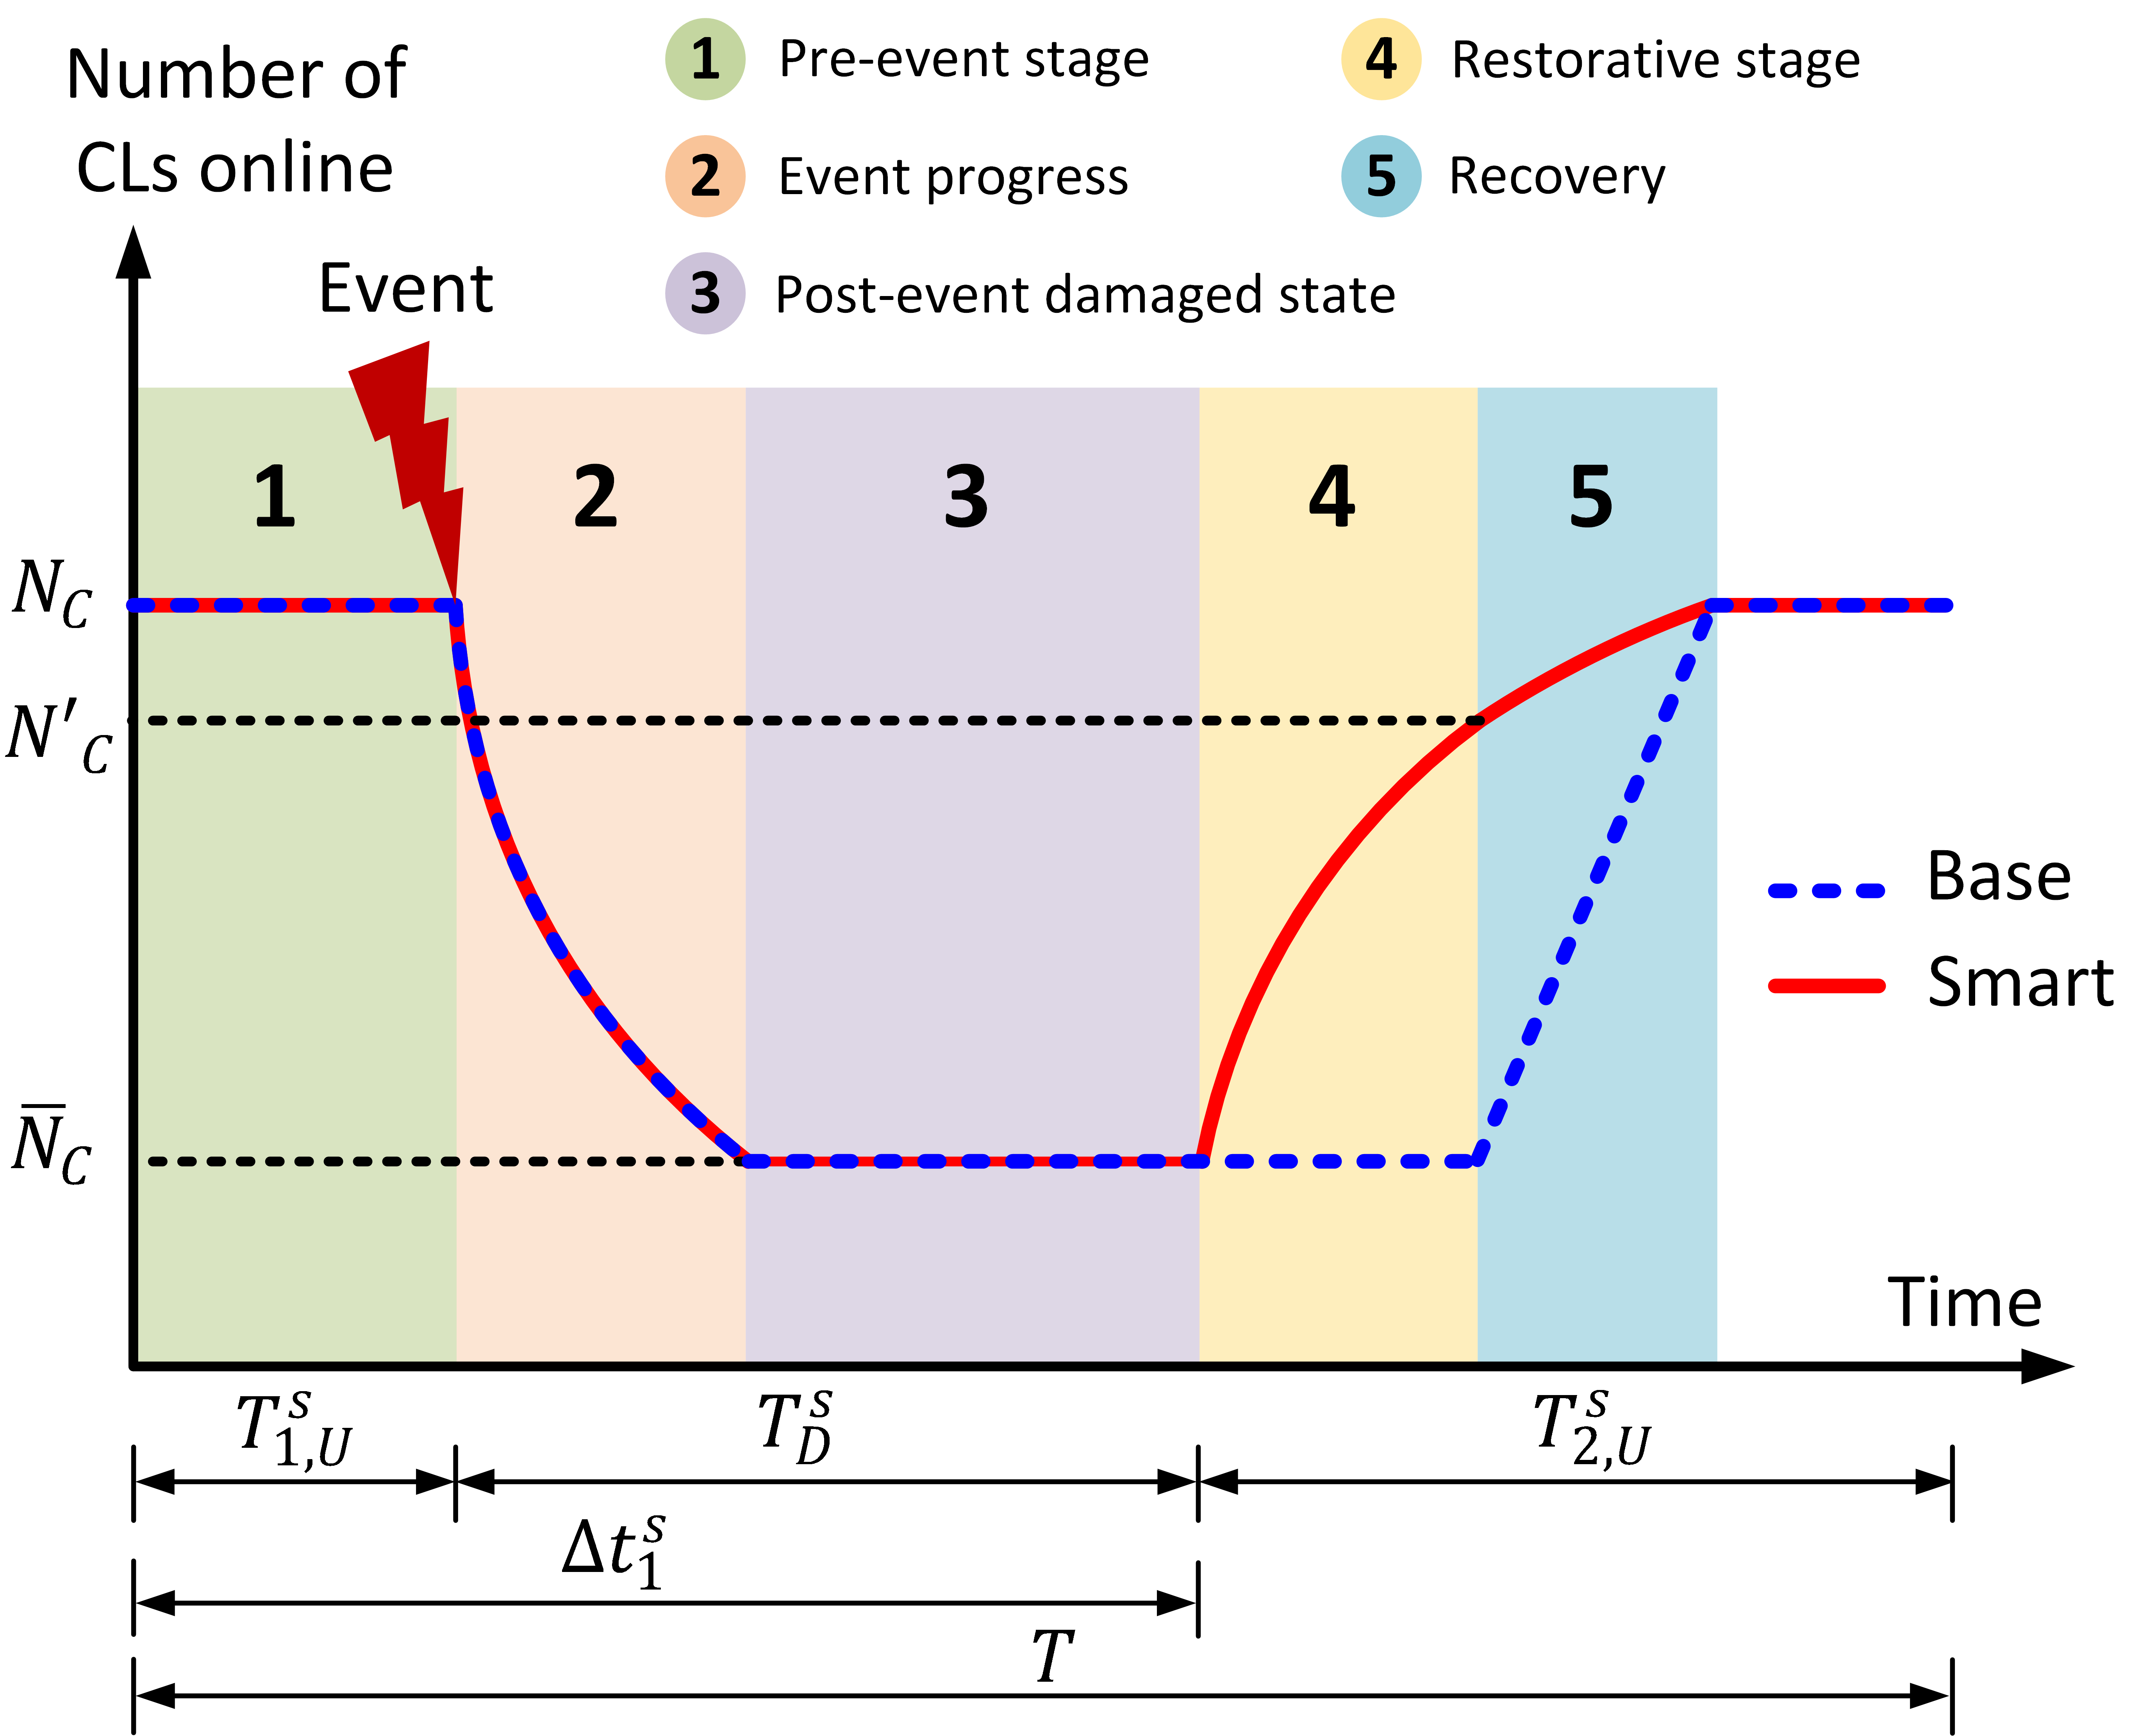
\includegraphics[width=0.65\textwidth]{figures/resilience_curve.png}
    \caption{Typical resilience assessment curve based on the number of weighted CL online. The time variables on the $x$-axis refer to the smart network~\cite{2016}.}
    \label{fig:resilience_curve}
\end{figure}

\paragraph{Resilience Parameters:}\label{par:resilience_parameter}

Fig.~\ref{fig:resilience_curve} shows a typical resilience assessment curve in which the $x$-axis represents time whereas the $y$-axis represents the number of weighted CLs online. Let $N_C$ be the total number of CLs that are online at a particular instance of time. The time in which all of the CLs remain online to the time an event occurs is denoted by $T_{1,U}$ and represented by phase 1. In this work, $T_{1,U}$ is considered the same for all CLs. The event occurs at the end of $T_{1,U}$ and sustains for a certain time. The time of event progress depends on the nature and intensity of the event and is denoted by phase 2 of the resilience assessment curve. Some CLs get disconnected due to the severity of the event. $\Bar{N}_C$ be the number of CLs that remain online after an event occurs. Phase 3 denotes the time for damage assessment. Smart networks have smart devices and damage assessment tools that can decrease the damage assessment time significantly. The CLs get disconnected when an event occurs until the point when repair or restoration starts. This is the downtime for CL and is denoted by $T_D$. $\Delta t_1$ is the period from the initial time to the time when repair/restoration begins. For the base case, the repair does not start until the recovery state, phase 5, whereas for the smart network DGs and remote-controlled switches (RCSs) can assist in load restoration, phase 4. At the point of repair/restoration, some of the CLs become online again and remain online for a time $T_{2,U}$. Let $N'_C$ be the number of CLs that are online after the load restoration phase. The total up and downtime of CL for the entire duration is represented by $T=T_{1, U} + T_D + T_{2,U}$. 

In this work, we only consider phases 1 through 4 for quantifying the resilience metric. We will discuss a few parameters that help us define the resilience of a distribution grid as referred to the critical loads and phases described in Fig.~\ref{fig:resilience_curve}. A detailed explanation of these parameters are given in~\cite{2016} while some of them are modified as necessary for this work.

\paragraph*{Availability:}

Let $i = 1, 2, ... ,N_C$ be the CLs connected in a system, $T_U^i = T_{1,U}^i + T_{2,U}^i$ be the time period when a CL $i$ is connected to system (up time), and $T_D^i$ be the time period when $i$ is disconnected from the system (down time) due to an extreme event. Hence, availability refers to the fraction of time when $i$ is online and is defined as:
\vspace{-3pt}
\begin{equation} \small
    \mathcal{R}_\psi = \frac{\sum_{i=1}^{N_C} T_U^i}{\sum_{i=1}^{N_C} (T_U^i + T_D^i)}
    \label{eq:availability}
\end{equation}

\noindent
Here, $T_U^i$ and $T_D^i$ for each $i$ depends on the type of network. For smart network, some disconnected CLs are restored in phase 4 which increases the overall availability of the system. Here, the choice of $N_C$ is problem specific and can represent a single customer as well as a particular feeder~\cite{2016}.   

\paragraph*{Robustness:}

Let $n_0$ be the number of CLs that are disconnected from the system at a given time. Then the outage incidence, $\theta$ is defined as:
\vspace{-5pt}
\begin{equation} \small
    \theta = \frac{n_0}{N_C}
    \label{eq:max_incidence}
\end{equation}

\noindent
If $N_C - \Bar{N}_C$ be the maximum number of CLs disconnected from the system and $\theta_{max}$ is the maximum outage incidence for a given time, then robustness is defined as:
\vspace{-3pt}
\begin{equation} \small
    \mathcal{R}_\beta = 1 - \theta_{max} = 1 - \frac{N_C - \Bar{N}_C}{N_C} = \frac{\Bar{N}_C}{N_C}
    \label{eq:robustness}
\end{equation}

% Robustness of a system is entirely dependent on the nature of the event and infrastructure of the system. Hence, this attribute is independent of the type of network --- Base or Smart.

\paragraph*{Brittleness:}

Let $D$ be the percentage of infrastructure damage in the system. For simplicity, we only consider distribution lines as infrastructures in this work. Brittleness is the level of disruption that occurred in the system with respect to damage. For instance, if the damage of a single distribution line affects the entire system then the system is highly brittle. The brittleness of a system with $N_C$ critical loads is defined as:
\vspace{-3pt}
\begin{equation} \small
    \mathcal{R}_\gamma = 100 \times \frac{\theta_{max}}{D}
    \label{eq:brittleness}
\end{equation}

\paragraph*{Resistance:}

According to~\cite{2016}, a system has higher resistance if it can withstand extreme events better and can operate the loads for a longer period before getting disconnected. With this notion, a resistant system should have better physical infrastructures, proper damage assessment methods, and situational awareness in case of extreme events. Furthermore, the resistance is also dependent on the nature of the extreme event. Here, $\sigma$ is the measure of an extreme event and is obtained as described in~\cite{2016}. Based on the measure of the event and time before which the repair and restoration begins, the resistance of a system is given by:
\vspace{-3pt}
\begin{equation} \small
    \mathcal{R}_\xi = \frac{\sigma \sum_{i=1}^{N_C} T_{1,U}^i}{\theta_{max} N_C \Delta t_1}
    \label{eq:resistance}
\end{equation}

\paragraph*{Resourcefulness:}

Let $N_{SW}$ be the number of tie-line switches, $N_S$ be the number of generating sources, and $N_P$ be the number of simple paths from each of the sources to CLs after an event has occurred in a network. Then the available resources are useful only if their existence is meaningful in system restoration. Thus, resourcefulness is defined as:
\vspace{-3pt}
\begin{equation} \small
    \mathcal{R}_\delta = \frac{N_P}{(N_{SW} + N_S) \times N_C}
    \label{eq:resourcefulness}
\end{equation}

For the base network, the only available source is the substation so $N_{S} = 1$ for the base case. For the smart network, $N_{S}$ increases as the number of DG increases. However, the resourcefulness decreases if those DGs are not utilized in network restoration after the event has occurred which is ensured by $N_C$. Thus, resourcefulness can be useful for planning the placement and number of DGs to enhance system resilience.

\paragraph{Risk Metrics:}

As discussed in~\cite{poudel2019risk}, we use $CVaR$ as a risk measure for each of the parameters. $VaR$ is defined as the specific threshold $\zeta$, such that with a specified probability of $\alpha$ $VaR$ does not exceed $\zeta$. On the other hand, $CVaR$ is the expected value of the distribution that exceeds $VaR$. Both of these metrics depend on the value of $\alpha$ and are commonly represented as $VaR_\alpha$ and $CVaR_\alpha$. If $p(I)$ be the probability distribution of a random weather event $I$ then the cumulative probability distribution that the parameter $\mathcal{R}$ will not exceed $\zeta$ when impacted by $I$ is given by:
\vspace{-5pt}
\begin{equation} \small
    \Psi (\zeta) = \int_{\mathcal{R}(I)\leq \zeta }^{} p(I) dI
\end{equation}

\noindent Thus, $VaR_\alpha$ and $CVaR_\alpha$ are then defined by:
\vspace{-5pt}
\begin{equation} \small
    VaR_\alpha (\zeta) = \inf\{\zeta \in \mathbb{R}:\psi(\zeta)\geq \alpha\}
    \label{eq:var}
\end{equation}
\vspace{-10pt}
\begin{equation} \small
    CVaR_{\alpha} (\zeta) = (1-\alpha)^{-1}\int_{\mathcal{R}(I)\geq VaR_{\alpha} }^{} \mathcal{R}(I)\ p(I)\ dI
    \label{eq:cvar}
\end{equation}

\noindent $CVaR_\alpha$ represents the value of parameter for the extreme $(1-\alpha)\%$ of impacts. It is also to be noted that the distribution of parameters below and above the specified threshold $\zeta$ represent the complete distribution of extreme events with a probability of $\alpha$ and $1-\alpha$ respectively.

\paragraph{Multi-criteria Decision Making using Choquet Integral:}
When it is essential to include multiple criteria in a decision making process then a single attribute or performance-based analysis do not accurately justify the decision. The Choquet Integral is an effective method for the MCDM problem~\cite{choquet} and is well suited for our framework.

If $\mu$ denote the fuzzy measure on $\Gamma$ then the discrete Choquet integral of a function $f:\Gamma\rightarrow\mathbb{R}^+$ with respect to $\mu$ is defined as~\cite{choquet}:
\vspace{-3pt}
\begin{equation} \small
    \mathcal{C}_\mu(f) := \sum_{i=1}^{n}(f(i)-f(i-1))\mu(\{\mathcal{R}_1, \mathcal{R}_2, .... , \mathcal{R}_n\})
    \label{eq:choquet}
\end{equation}

\noindent
where $f(.)$ are arranged in ascending order of its magnitude and is the $CVaR_\alpha$ of the parameters calculated using~(\ref{eq:cvar}), $\mu({\mathcal{R}})=\eta_\mathcal{R}$ is defined as the Shapely value which accounts for the behavioral analysis of any fuzzy measures, and $f(0) = 0$. More detail information on the Shapely value analysis and fuzzy measures is provided in~\cite{2006}. Choquet integral gives the overall score of alternative decisions in problem involving multiple parameters for each decision.

\subsubsection{Probabilistic Event and Impact Assessment}
Fig.~\ref{fig:ysys} shows the overall framework to quantify the system resilience using a stochastic simulation-based approach and is described in detail below. It is to be noted that the smart network contains DG-based restoration and RCS that can improve the damage assessment and restoration phase to enhance the overall resilience of the system.   
\begin{figure*}[t]
    \centering
%    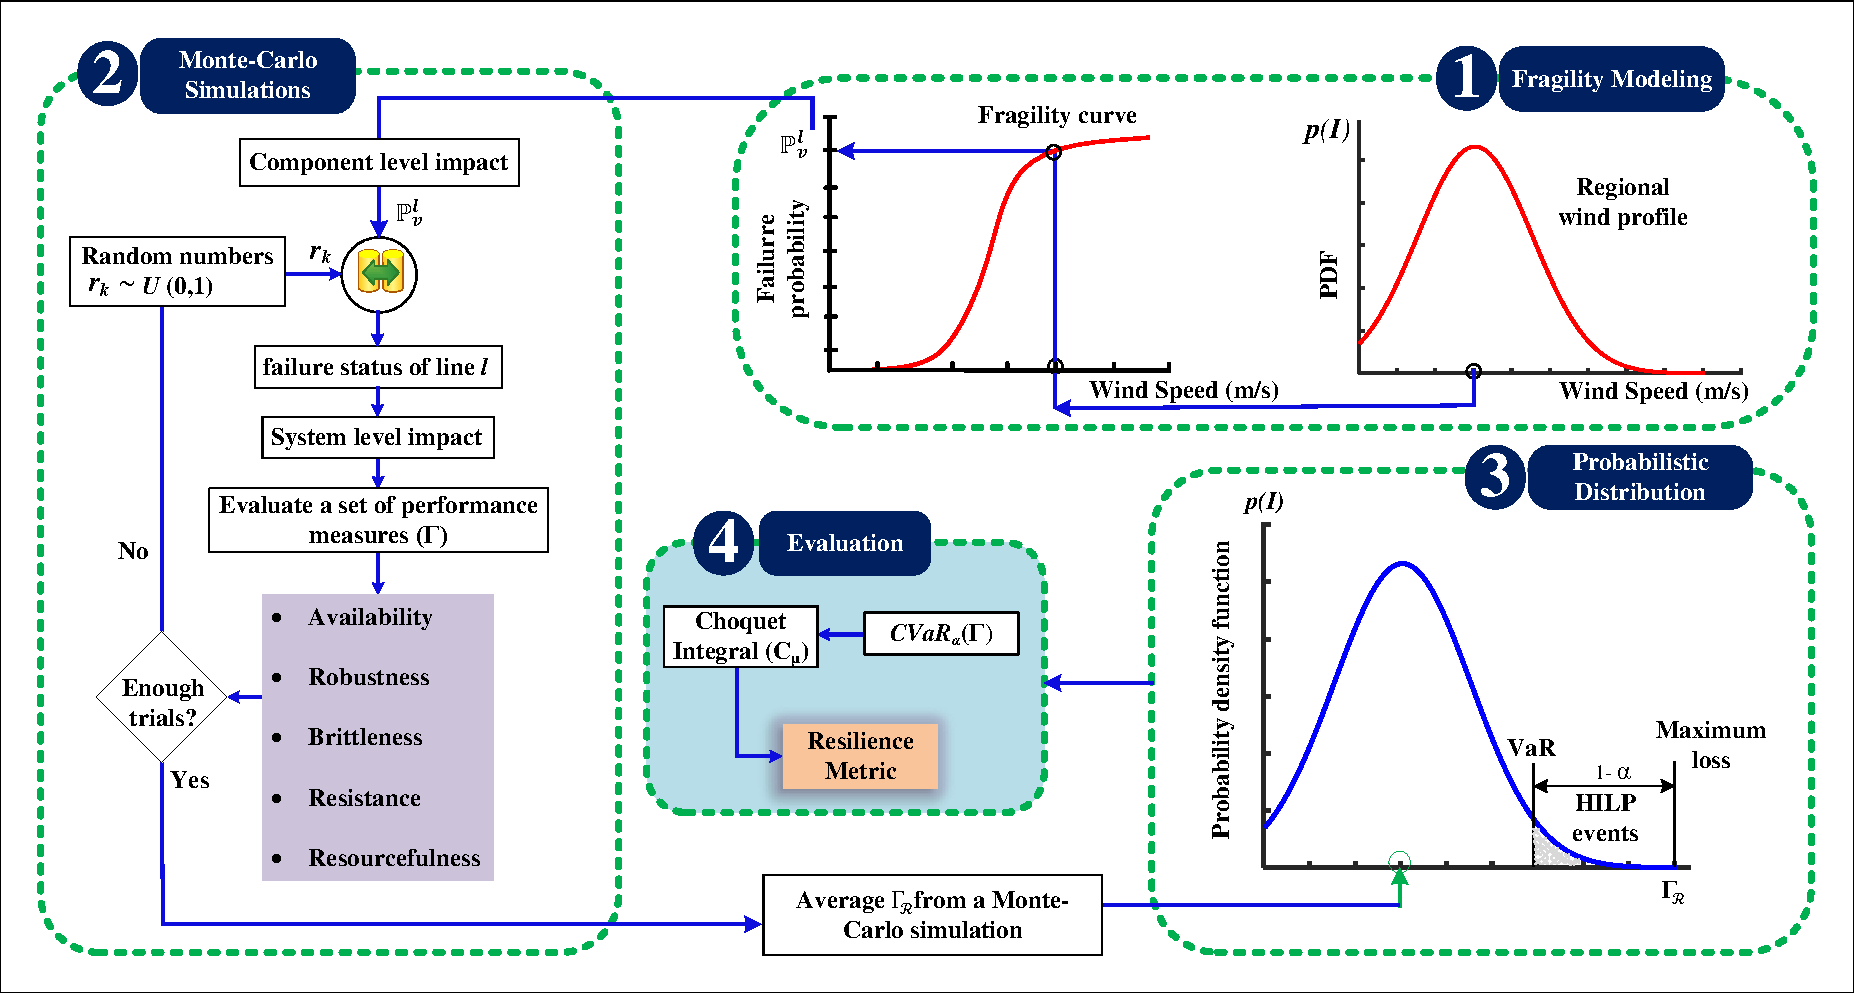
\includegraphics[width=0.9\textwidth,trim={0.5cm 0.25cm 0.35cm 0.5cm}, clip] {figures/MCS.pdf}
    \vspace{-0.2 cm}
    \caption{Simulation-based framework for resilience metric computation; Fragility modeling feeds the failure probability to Monte-Carlo simulation. Monte-Carlo simulation calculates the average value of a performance measure for a given event. $CVaR_\alpha$ is then calculated using the pdf of a given extreme event case.}
    \label{fig:ysys}
    \vspace{-0.3 cm}
\end{figure*}

The extreme wind event and its impact is characterized using its probability distribution and line fragility model. The fragility model of any distribution line gives the outage probability of the line subjected to a particular wind speed and can be represented as:
\vspace{-5pt}
\begin{equation} \small 
\begin{aligned}
&\mathbb{P}_v^l= \begin{dcases}\mathbb{F}_n^l & v < v_{cri} \\
\mathbb{P}^l (v)  & v_{cri} \leq v < v_{col} \\
1 & v \geq v_{col} 
\end{dcases} \\
\end{aligned}
\label{eq:outage}
\vspace{-3pt}
\end{equation}
where $\mathbb{F}_n^l$ is the failure rate of line $l$ in normal weather condition, $\mathbb{P}^l (v)$ is the failure probability of line $l$ as a function of $v$, $v_{cri}$ is the critical wind speed at which line $l$ experiences failure, and $v_{col}$ is the wind speed threshold beyond which line $l$ is guaranteed to fail. Since the process of identifying an event and its impact is purely stochastic, Monte-Carlo simulations are conducted to evaluate the probabilistic impacts of the event on the power distribution grid. The approach is generic as each event is simulated for several trials. The fragility models provide the failure probability of any distribution lines. With the increase in wind intensity, the failure probability increases accordingly. Monte-Carlo simulations help us identify the number of lines being failed in each trial, and resilience-driven parameters are evaluated using~(\ref{eq:availability}) -- (\ref{eq:resourcefulness}). For smart network, the optimization framework using DGs are modeled and simulated as described in~\cite{poudel2018critical}. In the optimization model, all the CLs are equally important and a weight factor of 10 is used for CLs and 1 for non-CLs. At the end of each simulation, the average of evaluated parameters for all trials is then mapped with the respective intensity of the events to form a distribution of each parameter corresponding to its intensity. 

The probability distribution of each of the parameters corresponds to the distribution of the intensity of the event. Thus, $CVaR_\alpha$ of each of the parameters can be calculated using~(\ref{eq:cvar}). It is to be noted that the value of $\alpha$ is consistent for each of the parameters. To combine $CVaR_\alpha$ in the decision-making process, the priorities of each of the parameters are obtained from the system operators and Shapely values of those priorities are evaluated. Finally, based on the $CVaR_\alpha$ of each of the parameters and their Shapely values, Choquet Integral gives an overall score using~(\ref{eq:choquet}). To identify the interaction of each of the parameters, $\lambda$ is also considered in the overall calculation process. The overall score obtained from Choquet Integral is the resilience metric for the distribution system. The described process is holistic as it considers all of the resilience-driven parameters (both attribute-based and performance-based) with their priorities in a system along with the associated risk.  

\subsubsection{Preliminary Research Results}
The proposed method of resilience metric quantification using $CVaR_\alpha$ of multiple parameters and Choquet Integral is demonstrated on IEEE 123-bus test system, Fig.~\ref{fig:IEEE_123_testcase}. The simulation is carried out for extreme wind-related events. It was experimentally verified that 1000 trials are enough to achieve convergence of MCS for any wind speed scenarios.

\begin{figure}
    \centering
%    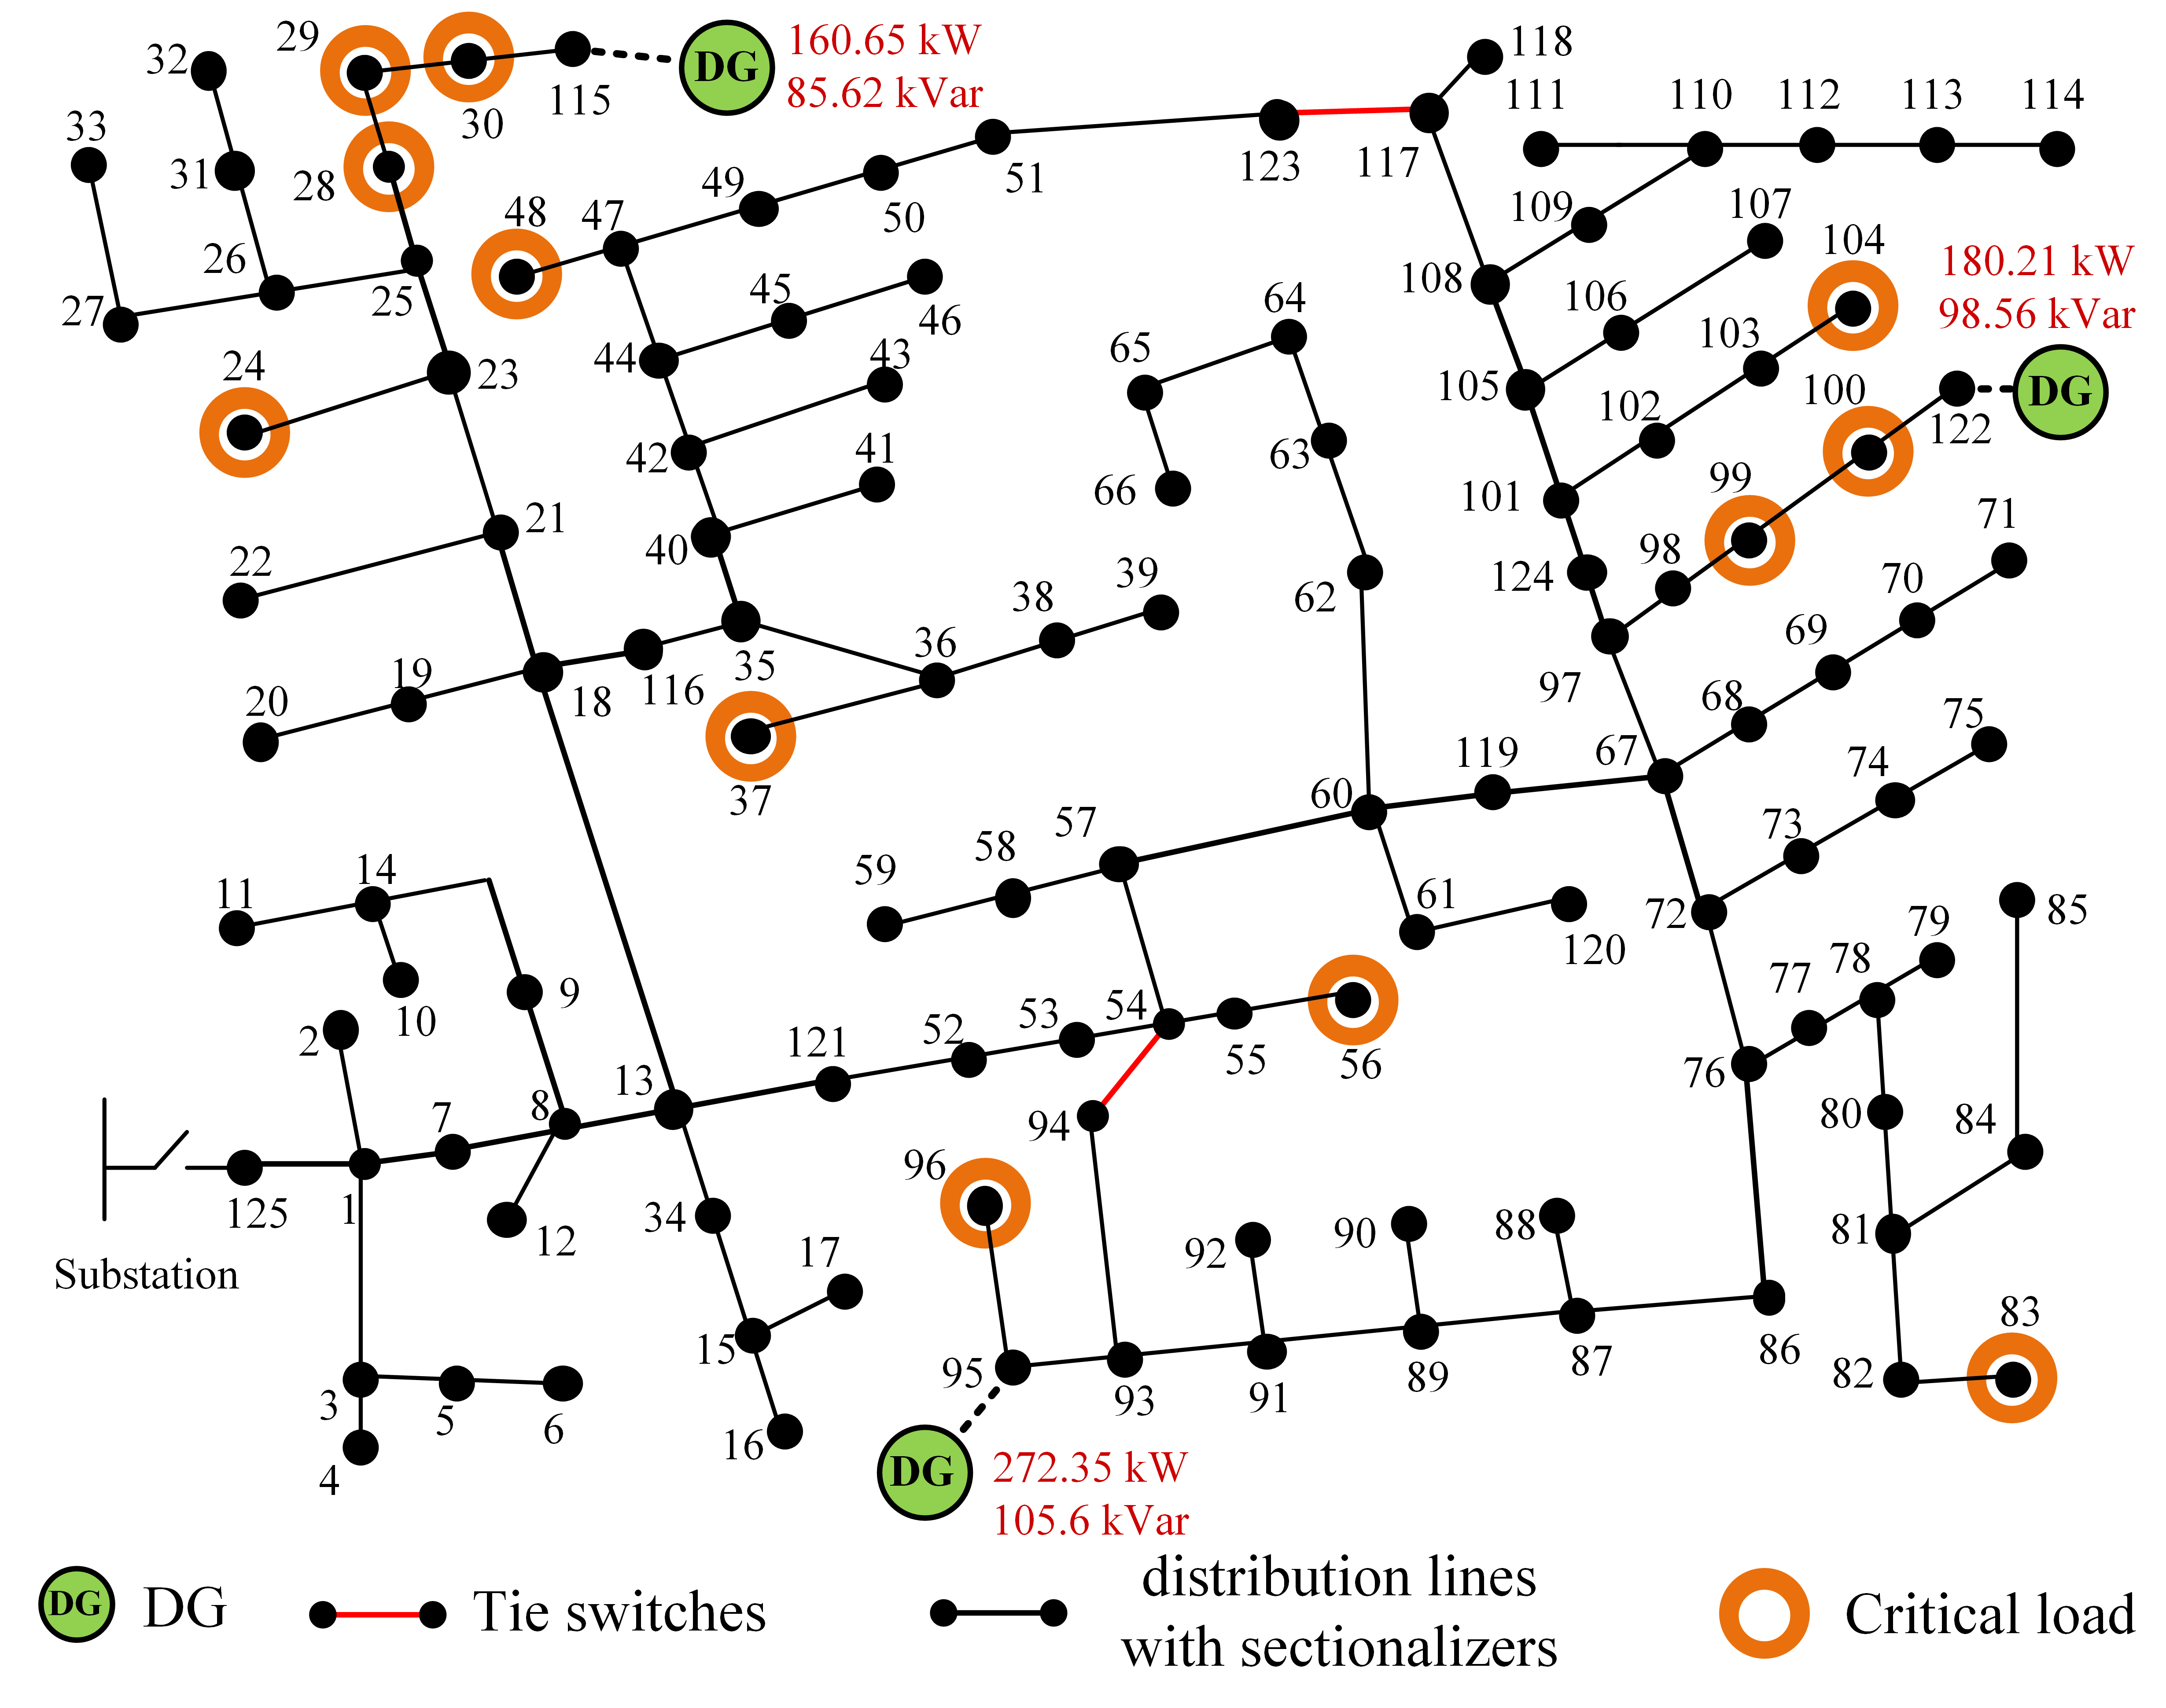
\includegraphics[width=0.55\textwidth]{figures/IEEE_123_testcase.png}
    \caption{Modified IEEE-123 test case with DGs, tie switches, and CLs.}
    \label{fig:IEEE_123_testcase}
\end{figure}

\paragraph{Calculating CVaR of Parameters:}
The five parameters defined in Section~\ref{par:resilience_parameter} are calculated based on Fig.~\ref{fig:resilience_curve} and using the simulation method described above. Fig.~\ref{fig:availability} shows the PDF of $\mathcal{R}_\psi$ obtained for each wind speed along with $VaR_\alpha$ and $CVaR_\alpha$ values. For all of the cases, the value of $\alpha$ is set to be 0.95. The $VaR_\alpha$ and the $CVaR_\alpha$ are calculated using~(\ref{eq:var}) and~(\ref{eq:cvar}). The risk metrics for other parameters are calculated in a similar fashion and are shown in Table~\ref{tab:CVAR}. Each of the parameters are normalized using min-max normalization technique for generality.  

\begin{figure}
    \centering
%    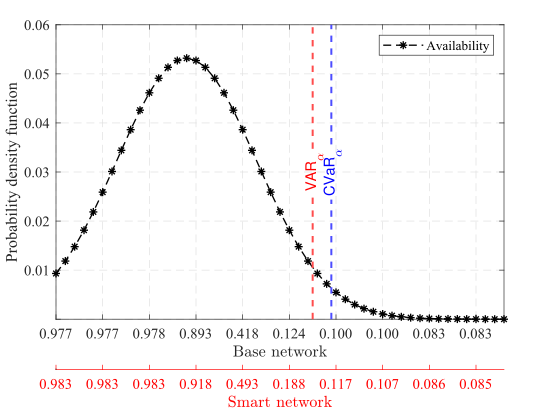
\includegraphics[trim=0cm 0.3cm 1.45cm 0.5cm,clip,width=0.55\textwidth]{figures/Availability.png}
    \vspace{-5pt}
    \caption{PDF of availability for base and smart network.}
    \label{fig:availability}
\end{figure}


%%%%%%%%%%%%%%%%% table for CVaR values %%%%%%%%%%%%%%%%%%%%%
\begin{table}[h]
    \centering
    \caption{$CVaR_\alpha$ of normalized resilience-based \\ parameters for base and smart network}
    \begin{tabular}{c|c|c|c|c|c}
    \hline
          Cases & $\mathcal{R}_\psi$ & $\mathcal{R}_\beta$ & $\mathcal{R}_\gamma$ & $\mathcal{R}_\xi$ & $\mathcal{R}_\delta$  \\
    \hhline{======}
         Base & 0.01115 & 0.00012 & 0.01656 & 0.0037 & 0.00005 \\
    \hline
         Smart & 0.01932 & 0.00012 & 0.01656 & 0.0039 & 0.00314 \\ 
    \hline
    \end{tabular}
    \label{tab:CVAR}
\end{table}



\paragraph{Quantifying Resilience using Choquet Integral:}
To compute the resilience metric based on the multiple parameters and their respective importance, five different cases are developed. For each of the cases, $\mu(.)$ is assigned for each parameter as shown in Table~\ref{tab:weights}. These are the initial fuzzy weights given by the experts or system operators that indicate the priority of one parameter over others.   


%%%%%%%%%%%%%%%%% table for initial weights %%%%%%%%%%%%%%%%%%%%%
\begin{table}[h]
    \centering
    \caption{Initial fuzzy weights of parameters \\ for resilience metric calculation}
    \begin{tabular}{c|c|c|c|c|c}
    \hline
          Cases & $\mu(\mathcal{R}_\psi)$ & $\mu(\mathcal{R}_\beta)$ & $\mu(\mathcal{R}_\gamma)$ & $\mu(\mathcal{R}_\xi)$ & $\mu(\mathcal{R}_\delta)$  \\
    \hhline{======}
        I & 0.9 & 0.25 & 0.15 & 0.6 & 0.85 \\
    \hline
        II & 0.6 & 0.5 & 0.45 & 0.5 & 0.6 \\ 
    \hline
        III & 0.3 & 0.8 & 0.85 & 0.6 & 0.2 \\ 
    \hline
        IV & 0.9 & 0.6 & 0.6 & 0.6 & 0.2 \\ 
    \hline
        V & 0.2 & 0.6 & 0.6 & 0.6 & 0.9 \\ 
    \hline
    \end{tabular}
    \label{tab:weights}
\end{table}

Table~\ref{tab:shapely} shows the Shapely value of each of the parameters as obtained from their initial fuzzy weights. These values also indicate the marginal contribution of each of the parameters in the respective cases. For instance, in Case I the importance of $\mathcal{R}_\psi$ and $\mathcal{R}_\delta$ are greater than the importance of other parameters. Hence, these two parameters contribute more towards resilience quantification than the others. For different cases, the marginal contribution of each of the parameters differ according to the priority set by the system operator or expert.


%%%%%%%%%%%%%%%%% table for Shapely values %%%%%%%%%%%%%%%%%%%%%
\begin{table}[h]
    \centering
    \caption{Shapely values of each parameters \\ based of their initial weights.}
    \begin{tabular}{c|c|c|c|c|c}
    \hline
          Cases & $\eta_{\mathcal{R}_\psi}$ & $\eta_{\mathcal{R}_\beta}$ & $\eta_{\mathcal{R}_\gamma}$ & $\eta_{\mathcal{R}_\xi}$ & $\eta_{\mathcal{R}_\delta}$  \\
    \hhline{======}
         I & 0.35235 & 0.07617 & 0.04451 & 0.20400 & 0.32294 \\
    \hline
         II & 0.23225 & 0.18573 & 0.16404 & 0.18573 & 0.23225 \\ 
    \hline
         III & 0.09441 & 0.30385 & 0.33202 & 0.20849 & 0.06121 \\ 
    \hline
         IV & 0.34422 & 0.19903 & 0.19903 & 0.19903 & 0.05869 \\ 
    \hline
         V & 0.05869 & 0.19903 & 0.19903 & 0.19903 & 0.34422\\
    \hline
    \end{tabular}
    \label{tab:shapely}
\end{table}

%%%%%%%%%%%%%%%%% table for Choquet Integral %%%%%%%%%%%%%%%%%%%%%
\begin{table}[h]
    \centering
    \caption{Choquet Integral values based on \\ Shapely values of each parameters}
    \begin{tabular}{c|c|c|c|c|c}
        Network & Case I    &   Case II   & Case III & Case IV & Case V  \\
    \hhline{======}
        Base  & 5.45 & 6.03 & 7.36 & \textbf{7.89} & 4.72 \\
    \hline
        Smart & 9.36 & 8.68 & 8.36 & \textbf{10.93} & 6.31 \\ 
    \hline
    \end{tabular}
    \label{tab:CI_resilience}
\end{table}

The Choquet Integral values for the base and the smart network and each of the cases are shown in Table~\ref{tab:CI_resilience}. It can be seen that the resilience of the smart network is always greater than that of the base network regardless of individual test cases due to the presence of DGs. However, the resilience for individual networks varies with the Shapely values of each of the parameters. For instance, if we look at the smart network, Case IV is more resilient than any of the other cases as higher priority is given to load availability and infrastructural investments (i.e., $\mathcal{R}_\beta$, $\mathcal{R}_\gamma$, and $\mathcal{R}_\xi$). However, this is not true for the base network as loads are not picked up during the restoration phase in the base network making its availability lower than the smart network. It is also interesting to notice that, the resilience for Case I and Case IV does not have a huge difference although for Case I, the priority towards infrastructural investment is less. Hence, the operators can have the flexibility to focus more on less expensive decisions and still enhance the system's resilience.       


%%%%%%%%%%%%%%%%%%%%%%%%% NEXT CHAPTER %%%%%%%%%%%%%%%%%%%%%
\newpage
\subsection{Risk-based Resilience Planning of Power Distribution Systems}
\subsubsection{Prior work on Power Distribution Planning and their limitations}
The existing literature on power distribution resilience includes numerous articles on operational planning to mitigate or reduce the impact of an imminent threat such as an upcoming storm~\cite{8409997}. Such solutions build resilience via operational response rather than infrastructural upgrades. In operational planning, the decisions are to be made for an upcoming event that is known with a high level of certainty and thus requires considering only a limited number of scenarios for decision-making. On the contrary, long-term planning requires a probabilistic analysis over a wider range of scenarios with a higher level of uncertainty for decisions related to system hardening, infrastructure upgrades, resource allocation, and sizing ~\cite{7381672}. These decisions must also connect to the operational problem if and when the events are realized in practice. Thus, the problem is further complicated by additional stages of operational decision-making leading to an explosion of state space to be considered for decision-making. 

The related literature on resilience-oriented design and pre-disaster resource allocation usually employ a stochastic programming model to minimize the expected cost of the future operational scenarios  \cite{gao2017resilience , zhang2021stochastic}. For example, in \cite{gao2017resilience}, a heuristic search is employed to identify the optimal restoration path and obtain a resource allocation plan. These solutions, however, consider short-term operational requirements for a known HILP event and are not suitable for infrastructure planning. The related work on resilience-oriented distribution system long-term planning also employs stochastic optimization formulations, including a tri-level robust optimization model \cite{yuan2016robust, wang2018resilience}, and a two-stage stochastic optimization model \cite{ma2018resilience, ma2019resilience, liu2019unified}. The tri-level optimization model formulates the resulting problem in a defender-attacker-defender model that is then converted into an equivalent bi-level model and solved using iterative approaches such as CCG or greedy search algorithms~\cite{yuan2016robust}. The tri-level approach optimizes for the worst possible outcomes and hence is not suitable for a probabilistic analysis for infrastructure planning that needs to be cost-effective and optimal for a large range of future scenarios. Alternatively, the two-stage stochastic programming method considers the overall impact of stochastic fault scenarios in planning decisions rather than just the worst-case scenarios \cite{ma2018resilience, shi2020resilience}. The existing two-stage stochastic optimization formulations used in resilience-oriented distribution grid design either assume that all scenarios are observed with equal probability or perform the planning based on only a targeted set of scenarios~\cite{2021IASTATE, 8329529, 9136725}. While such methods are generally applicable, other approaches such as importance sampling and stratified sampling techniques can be more effective in representing HILP events and their impact probabilities in the optimization process~\cite{glynn1989importance, rush2000stratified}. These techniques are widely adopted in power systems reliability studies~\cite{8887536, 7084698}. For a resilience-oriented long-term planning problem, the goal is to determine optimal investments to reduce the consequences (here, customer outages) of the HILP events. Mathematically, this amounts to minimizing the mean of consequences and, more importantly, reducing the tail of the consequence of the HILP events~\cite{9120304}.


%%%%%%%%%%%%%%%%%%%%%%%%% NEXT CHAPTER %%%%%%%%%%%%%%%%%%%%%
\newpage

\begin{enumerate}
    \item \textit{Risk-averse Two-stage Stochastic Programming for Distribution Grid Resilience:} The two-stage stochastic programming problem is formulated as a MILP problem where Stage-1 decisions are the infrastructure planning decisions optimized to reduce the risks of outages due to HILP events assuming optional operational phase decisions.
    \item \textit{Probabilistic scenario generation and smart scenario reduction strategy:} A Monte-Carlo-based probabilistic scenario generation framework and smart scenario selection strategy is proposed to reduce the large scenario samples to representative scenarios.
    \item \textit{Trade-off analysis on risk minimization vs. expected loss minimization:} Different case studies are presented to identify the trade-off of adopting risk-neutral vs. risk-averse policies in the planning decisions. The analysis can provide insights into adopting risk-driven solutions when the utmost priority is to maintain an uninterruptible power supply to critical customers during extreme weather events.
\end{enumerate}

\subsubsection{Planning Problem Representation}

A power distribution network can be graphically represented as $G(V,E)$, where the vertices $V$ represent the buses or nodes while the distribution lines are represented by the edges $E$. The overall objective of the two-stage framework is to identify the first-stage optimal planning decisions that minimize the expected operational cost in the second stage. In this work, DG siting and sizing are the planning decisions whereas the second stage objective is to minimize the prioritized load loss once a scenario is realized. DGs with grid-forming inverters are assumed in this work. Such grid-forming DGs can be used for intentional islanding when some area of the distribution grid gets disconnected from the system due to an extreme event. 

The two-stage objective function is a random variable. Thus, determining the optimal planning decision is the problem of comparing random cost variables as a function of the planning cost and the operational cost. The overall problem is formulated as a risk-averse stochastic optimization problem in which the first stage problem minimizes the cost of planning and the weighted combination of the expected value and the $CVaR$ of the second stage problem. The second stage problem is the operational stage that minimizes the total prioritized loss of load for every scenario realization.
    
    \begin{figure}[t]
        \centering
        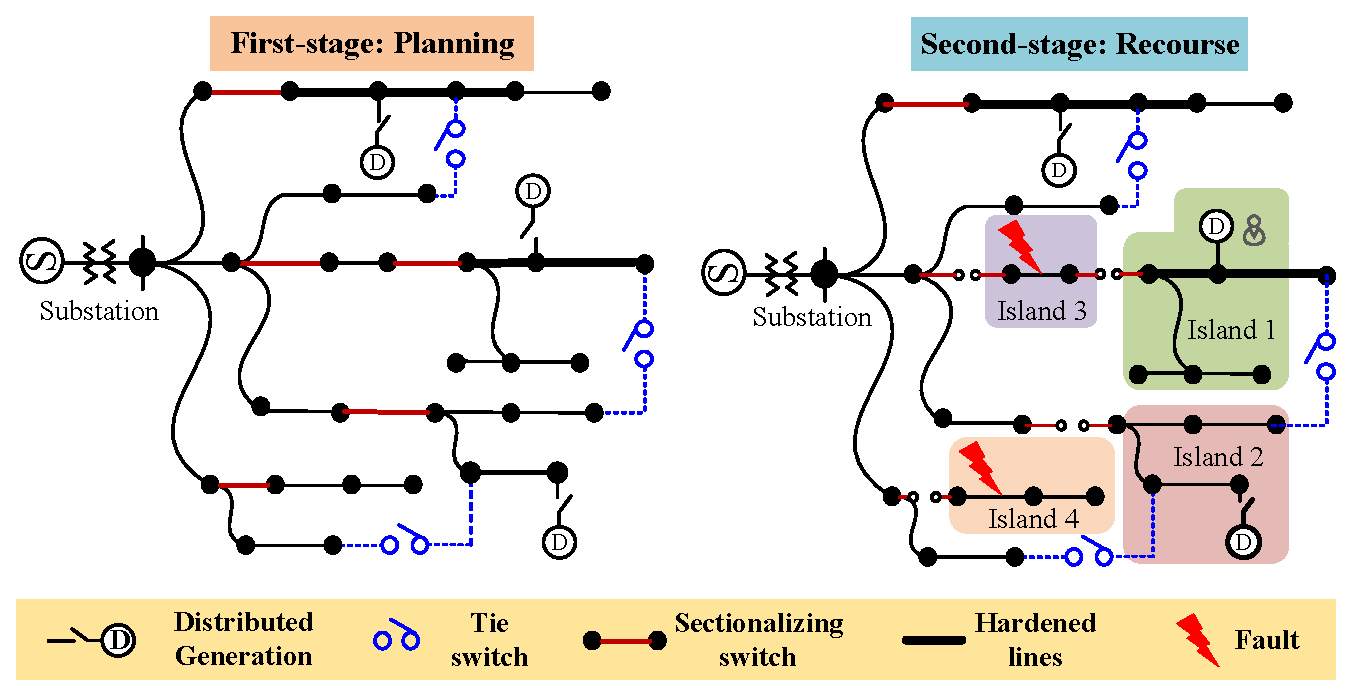
\includegraphics[width=0.75\textwidth]{figures/first_second_stage_model.eps}
        \caption{Two-stage planning framework example for a specific scenario.}
        \label{fig:model_representation}
    \end{figure}

\subsubsection{Problem formulation}
The resilience-driven distribution system planning problem is formulated as a two-stage stochastic optimization problem where the overall objective function can be defined as:

\begin{equation}
\small
    \begin{split}
    \min (1-\lambda)\mathbb{E}(Q(\delta, \mathcal{E})) + \lambda CVaR_\alpha(Q(\delta, \mathcal{E}))
    \end{split}
    \label{eq:main_objective}
\end{equation}
where,
\vspace{-5pt}
\begin{equation*}
\small
    \begin{gathered}
        \mathbb{E}(Q(\delta, \mathcal{E})) := \left(\sum_{\xi \in \mathcal{E}}\sum_{i\in  \mathcal{B}_S}\sum_{\phi\in\{a,b,c\}}(1 - s^\xi_i)\ w_i\ P_{Li}^{\phi,\xi}\right)\\
        CVaR_\alpha(Q(\delta, \mathcal{E})) := \left(\eta + \frac{1}{1-\alpha}\sum_{\xi \in \mathcal{E}}p^\xi\nu^\xi\right)
    \end{gathered}
\end{equation*}

The problem objective in the first stage is to minimize the weighted sum of expected value and $CVaR_\alpha$ of the second stage cost, represented by $Q(\delta, \mathcal{E})$. To analyze the trade-offs, this formulation has not used minimization of planning cost. Instead, we use a budget constraint and observe the associated trade-offs for risk-averse and risk-neutral decisions when system planners have a limited investment budget. The objective of the second stage of the problem, $Q(\delta, \mathcal{E})$, is to minimize the prioritized load loss or maximize the restoration of prioritized loads for each $\xi \in \mathcal{E}$. The second stage costs correspond to the optimal restoration decisions once a scenario has been realized. Hence, each variable corresponding to the second stage of the problem is scenario-dependent. $P_{Li}^{\phi,\xi}$ represents the active power demand at node $i$ for phase $\phi$ and scenario $\xi$ and $s_i^\xi \in {0, 1}$ is the load pick-up status variable that determines whether the load at node $i$ is picked up or not. The CLs are prioritized by a weight variable $w_i$. Since the CLs are critical for any scenario, $w_i$ remains the same for all scenarios. Furthermore, the scenarios have a specific probability, $p_\xi$, associated with them, which comes from the scenario reduction method discussed before. For the expression $CVaR_\alpha(Q(\delta, \mathcal{E}))$, $\nu_\xi$ is an excess variable which ensures that $CVaR_\alpha$ is calculated only for realizations beyond $VaR_\alpha$ for each scenario $\xi$. 

Here, DG location ($\delta^{DG}_i$) and size of the DG ($\beta^{DG}_i$) are the first stage decision variables. In this work, the per unit cost for DG installation and sizing is assumed to be the same for each location; these assumptions can be easily relaxed.  
Constraint (\ref{eq:DG_size}) ensures that the total cost of DGs should be between \$[0, $\mathcal{C}^{DG}_{max}$] regardless of the cost of installation in an individual location. This gives the freedom of utilizing the overall budget for a single big-sized DG or distributing the budget to multiple smaller-sized DGs. Constraint (\ref{eq:DG_size}) contains a non-linear term $\delta_i^{DG} \times \beta^{DG}_i$ which is linearized using big-M method as discussed in~\cite{coelho2013linearization}. Constraint (\ref{eq:DG_location}) restricts the DG location variable to binary. The DG location variable $\delta^{DG}_i$ is 1 if a DG is located in node $i$, else 0. Furthermore, constraint (\ref{eq:VAR_constraint}) ensures that $VaR_\alpha$ for the distribution of load loss in the second stage is a real number. Furthermore, $VaR_\alpha$ is independent of scenarios and is obtained with the solution of the first stage. 

\begin{subequations}
\begin{equation}
\small
    \sum_{i\in \mathcal{B}_{DG}} c_i^{DG}\delta_i^{DG} \beta^{DG}_i \leq \mathcal{C}^{DG}_{max} \\
    \label{eq:DG_size}
\end{equation}
\vspace{-10pt}
\begin{equation}
\small
    \delta^{DG}_i \in \{0,1\} \\
    \label{eq:DG_location}
\end{equation}
\begin{equation}
    \small
    \eta \in \mathbb{R} \\
    \label{eq:VAR_constraint}
\end{equation}
\end{subequations}

\noindent The overall problem formulation can be summarized as:\\
\newcommand\tab[1][0.5cm]{\hspace*{#1}}
	\tab Objectives:\\
	\tab \tab1) Minimize weighted sum of expected value and $CVaR_\alpha$ of the second stage cost\\
	\tab Constraints:\\
	\tab \tab1) First-stage constraints (scenario independent)\\
	\tab \tab2) Second-stage constraints (secenario dependent)\\
	\tab \tab \tab a) Connectivity constraints\\
	\tab \tab \tab a) Three-phase unbalanced power flow constraints\\
	\tab \tab \tab c) Network operational constraints\\
	\tab \tab \tab d) DG operating constraints\\
	\tab \tab \tab e) $CVaR_\alpha$ constraints

\subsubsection{Proposed scenario generation and selection approach}
The overall architecture of the proposed method is shown in Fig.~\ref{fig:overall_architecture}. Only wind-related events are used in this work and the probability distribution of extreme wind events is considered to generate the scenarios. Monte Carlo simulations (MCS) are conducted to identify the impact of probabilistic events, and an appropriate scenario reduction method is implemented to identify representative scenarios. Finally, the planning problem is solved in a two-stage stochastic optimization setting based on a selected number of scenarios.

\begin{figure}[t]
    \centering
    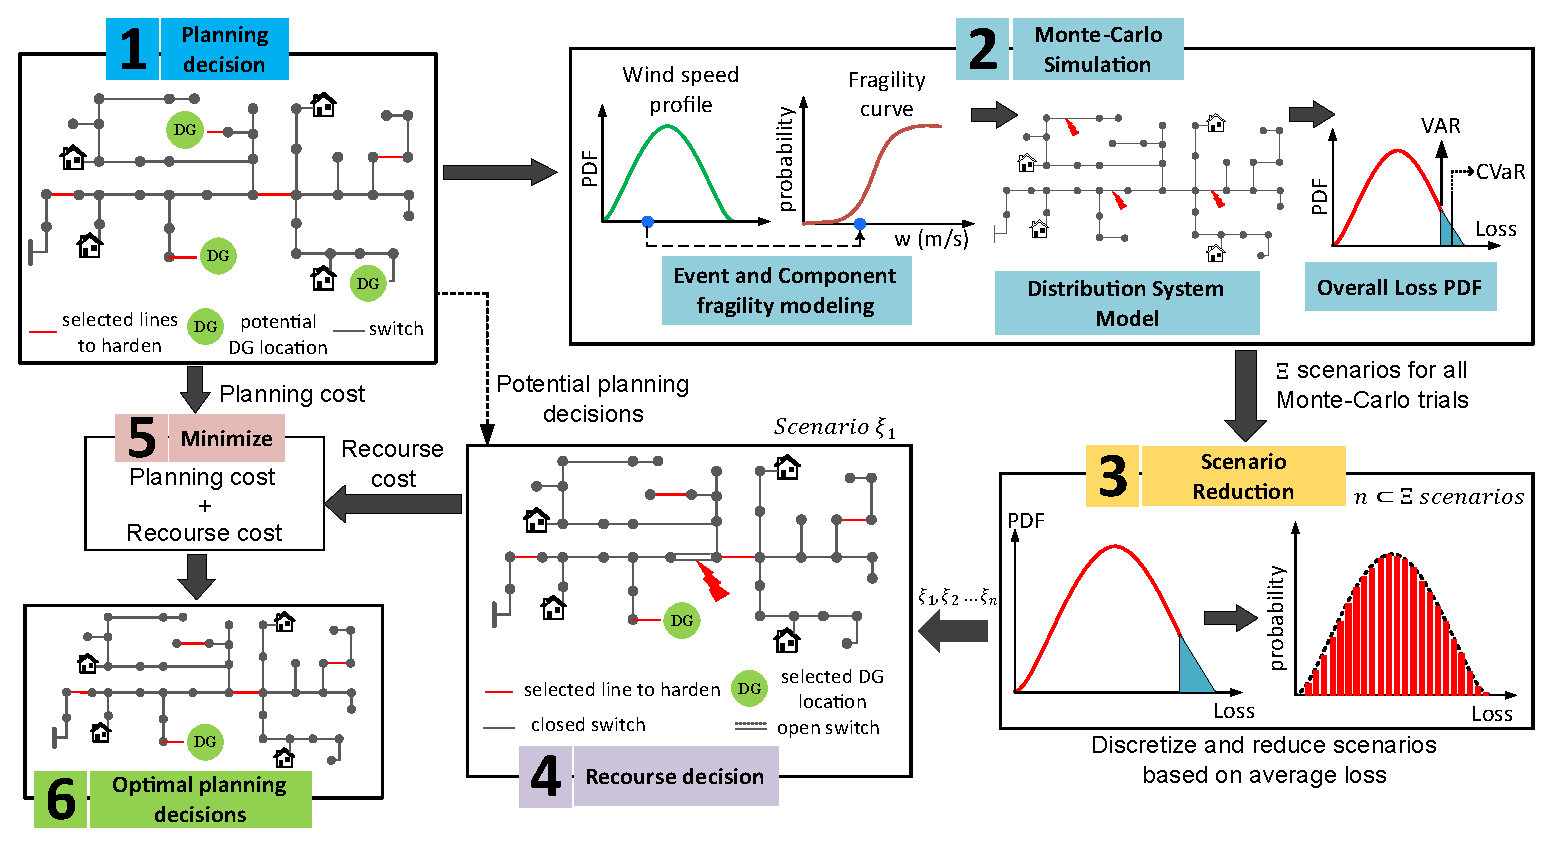
\includegraphics[width=0.8\textwidth]{figures/overall_picture.eps}
    \caption{Overall architecture of risk-averse two-stage planning problem. The first stage seeks the optimal planning decisions that minimize the expectation and risk of the recourse cost in the second stage for several scenario realizations. The scenarios are generated using Monte-Carlo simulation and reduced based on average loss for each scenario.}
    \label{fig:overall_architecture_framework}
\end{figure} 

\begin{figure}[h]
    \centering
    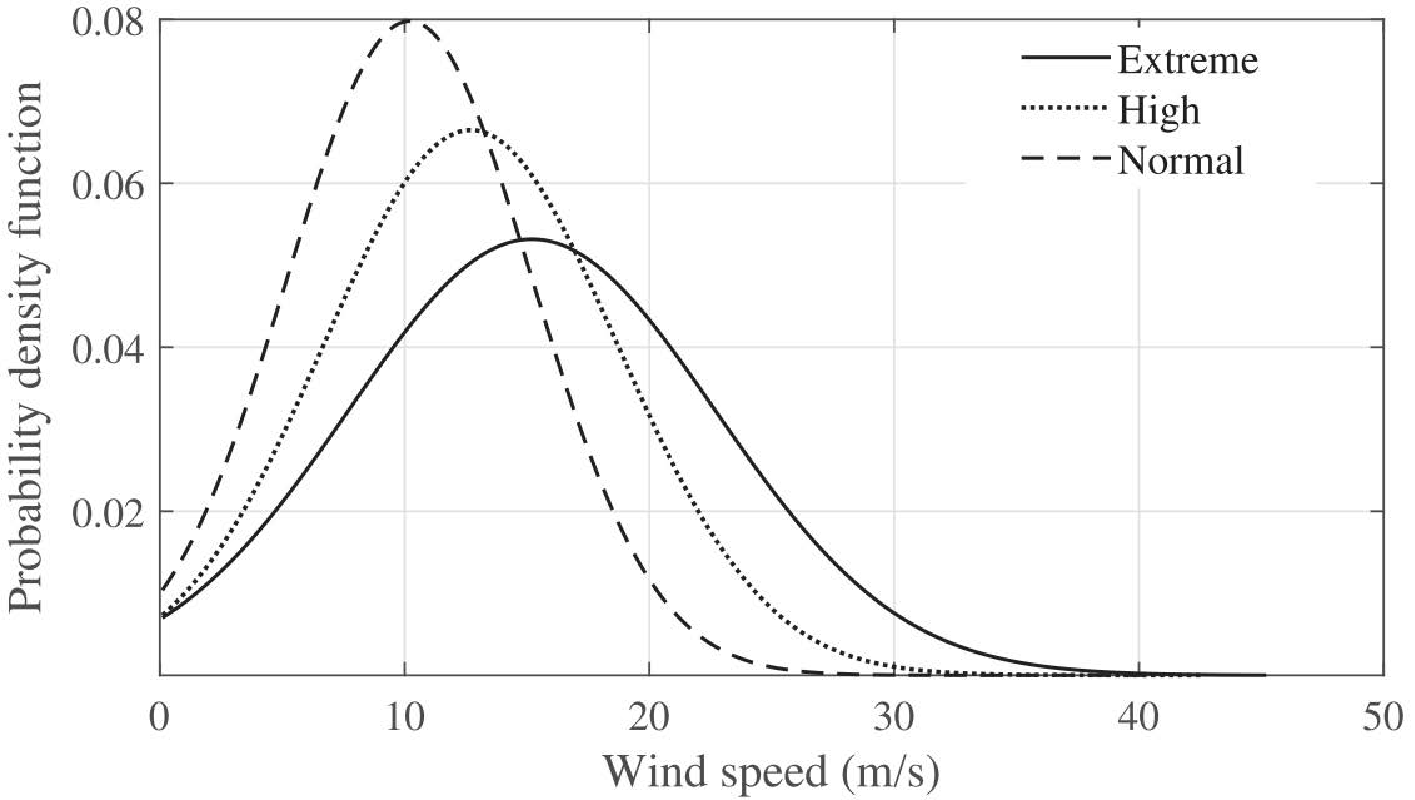
\includegraphics[width=0.7\textwidth]{figures/wind_profile.pdf}
    \caption{Regional wind profile.}
    \label{fig:wind_profile}
\end{figure}

Fig.~\ref{fig:wind_profile} shows the event probability distribution for a windfall in three different regions observing extreme, high, and normal wind profiles. The extreme regional wind profile is used to model extreme events in this work. For simplicity, only distribution lines are assumed to be affected by wind in this work. Although wind-related events have spatiotemporal dynamics~\cite{poudyal2021spatiotemporal}, we assume that for a distribution system, that covers a small region, the wind speed for the entire region is the same. MCS is performed for each wind speed case so as to also include the extreme tail probability events. This process is represented by block 2 in Fig.~\ref{fig:overall_architecture}. For each wind speed scenario $u$, the component level failure probability $p_f(u)$ determines the operational state of a particular component in the distribution grid. Component level fragility curves \cite{panteli2017power} or prototype curve fit models \cite{powell1995real} can be  used to model the impacts of extreme events such as hurricanes or other high-speed wind events on power systems. In this work, we have used the component fragility curve that maps the probability of failure of distribution system components conditioned on the intensity of the hazard (e.g., a wind speed). The fragility curve values are randomly selected for simulation purposes; however, if available, empirical data can be used to adjust the parameters~\cite{7036086}.

MCS provides an extremely large number of scenarios. One major challenge in any stochastic optimization setting is handling many scenarios within the optimization framework. Furthermore, the solution should be optimal for all scenarios that make the stochastic problem computationally intractable. Existing works use special sampling techniques such as stratified sampling~\cite{parsons2014stratified} or importance sampling~\cite{ekblom2020importance} to include the tail probability scenarios in the optimization model appropriately. Distance-based scenario reduction methods have also been used where a probabilistic distance measure is minimized to obtain a reduced scenario distribution that closely represents the overall scenario distribution~\cite{heitsch2007note}. We introduce a new approach to scenario reduction inspired by stratified sampling and distance reduction methods. The proposed approach uses stratification to sample representative scenarios for each wind speed and generates a reduced scenario distribution that closely matches the original scenario distribution.

In this work, the overall number of scenarios is reduced by selecting a representative scenario for each wind speed based on the average Monte-Carlo loss. This process is represented by block 3 in Fig. 3. Let $N_u$ be the total discrete wind speeds under consideration, $N_{\xi,u}$ be the number of scenarios obtained from MCS for each wind speed $u$, and $L^{u}_{avg} = \mathbb{E}(L_{\xi,u})$ be the average prioritized load loss in $kW$ corresponding to $N_{\xi,u}$ scenarios. Let $\Xi = N_{\xi,u} \times N_u$ be the total number of scenarios for the entire MCS. Note that we cannot randomly select a subset of these scenarios as it significantly degrades the accuracy of the optimization solutions. Here, we use a unique sampling technique to drastically reduce the number of scenarios while maintaining the representation of the overall scenarios described next. If $\xi_u$ is a representative scenario for all $N_{\xi,u}$ scenarios corresponding to $u$, then $\xi_u$ is selected such that the prioritized load loss in the system due to $\xi_u$ ($L^{u}_{\xi_u}$) is the one nearest to $L^{u}_{avg}$. In the case of multiple scenarios with losses nearing $L^{u}_{avg}$, one of the scenarios is randomly selected as $\xi_u$ from the identical scenario representations. The proposed scenario reduction technique reduces the total number of scenarios to $N_u$ from $\Xi$ such that $p_\xi$ corresponds to the wind speed profile. This smart scenario selection strategy ensures the practical realization of the second stage problem while incorporating HILP events within the scenarios. 

\subsubsection{Preliminary Research Results}
The effectiveness of the proposed risk-based long-term planning model is verified on a modified IEEE 123-bus case, see Fig.~\ref{fig:IEEE_123_testcase}. To analyze the planning decisions better, we create a new test case upon hardening 15 randomly selected lines, as shown in Fig.~\ref{fig:IEEE_123_testcase}. The fragility curves of hardened lines are adjusted so that their outage probability for any extreme event is less than the case when they are not hardened. For CLs, $w_i = 10$ whereas, for non-critical loads, $w_i = 1$. Thus the second stage cost reflects the total amount of prioritized loss of load (in kW). The total non-prioritized demand of the system is $P_D = 4485~kW$ and the prioritized demand is $\sum_{i\in\mathcal{V}}{w_iP_{Li}} = 20775~kW$. This work uses prioritized demand to analyze the results for different cases.

\begin{figure}[t]
    \centering
    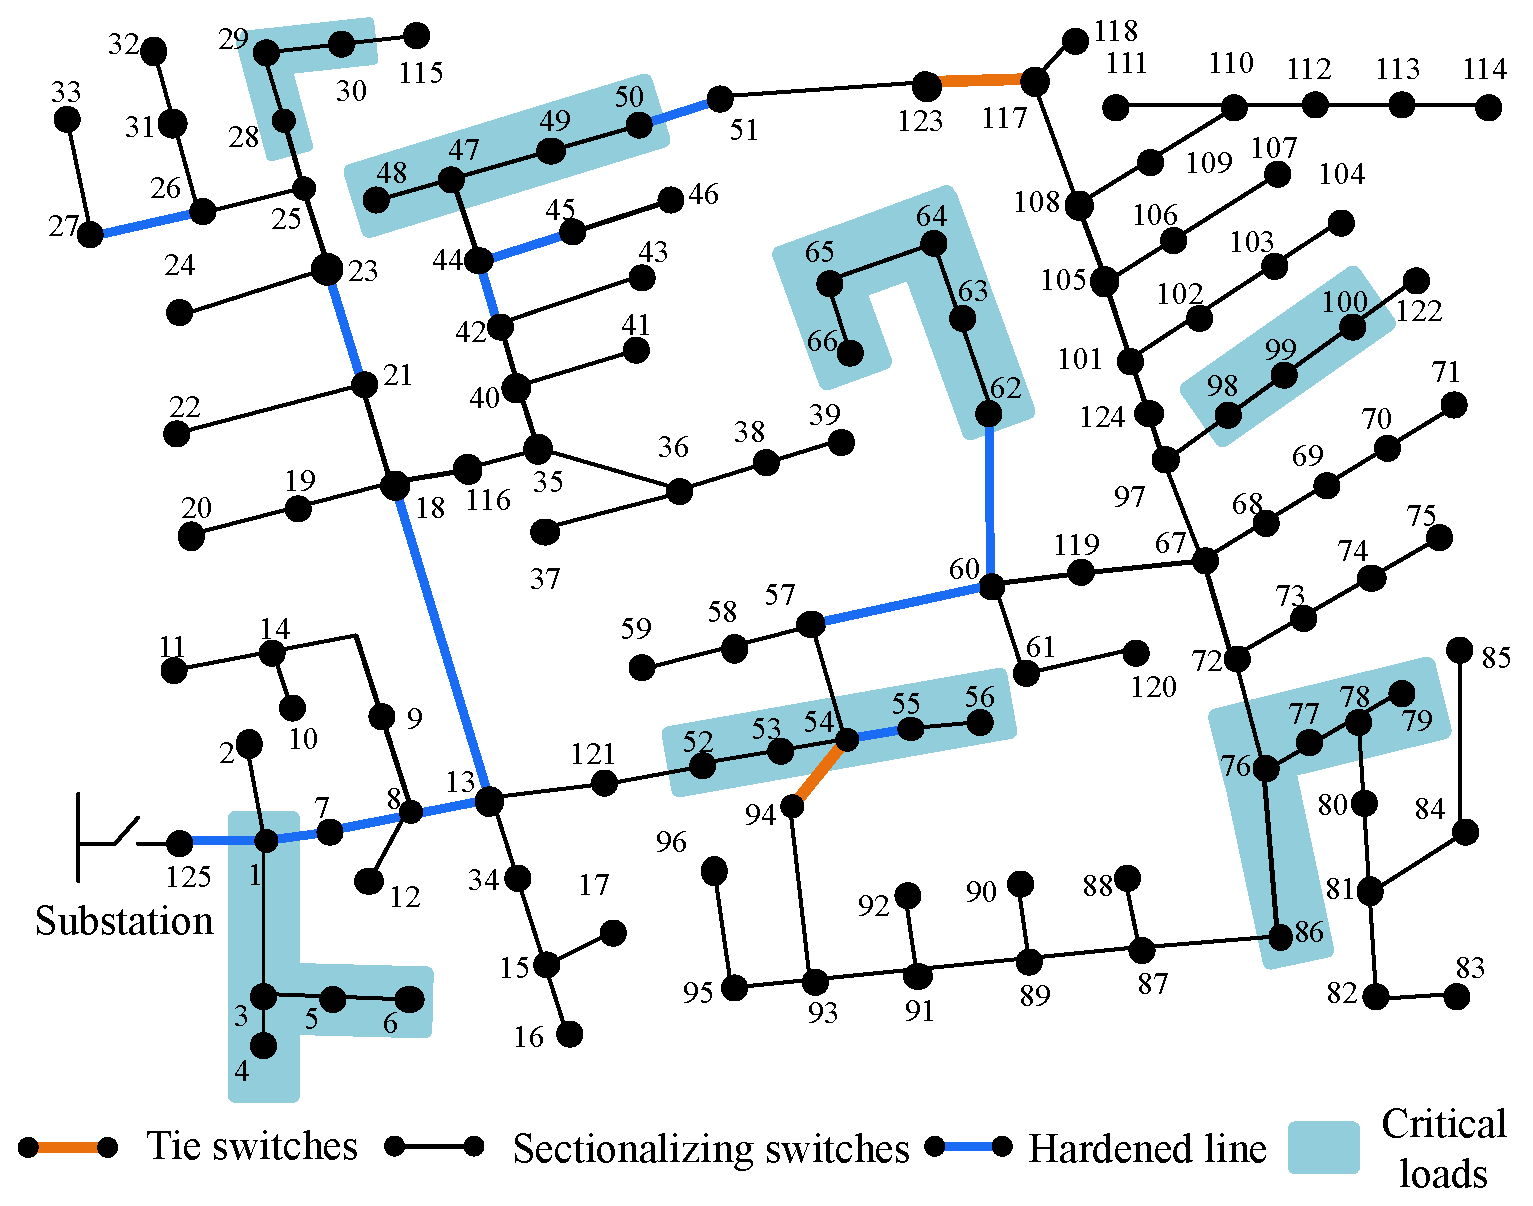
\includegraphics[width=0.7\textwidth]{figures/IEEE_123_CL_update.eps}
    \caption{Modified IEEE 123-bus test case}
    \label{fig:IEEE_123_CL_update}
\end{figure}

\paragraph{Scenario Generation and Reduction}
Using the wind speed profile for extreme wind events and failure probability of distribution lines, several trials of MCS simulation are conducted for sampled wind speeds~\cite{7036086}. For this experiment, $N_u=49$ wind speeds are sampled from the wind speed profile and it was experimentally verified that 1000 Monte-Carlo trials are enough to obtain a converged value of prioritized loss of load in the distribution grid corresponding to each $u$. Fig.~\ref{fig:MCS_convergence} shows the moving average of prioritized loss of load for 1000 Monte-Carlo trials for the base case without hardening and with hardening. It can be seen that the value of the loss is fairly converged in 1000 trials for both cases. Since 1000 trials are conducted for each $u$, $N_{\xi,u} = 1000$. Hence, the total number of scenarios generated through MCS, $\Xi = 49 \times 1000 = 49000$. 

Fig.~\ref{fig:scenario_reduction} represents the comparison between $L^u_{avg}$ and $L^u_\xi$ for the test case without hardening and with line hardening. The loss due to reduced scenarios is very close to that of the actual representative scenarios for each $u$. The y-axis on the right represents the value of $|L^u_{avg} - L^u_\xi|$. It can be seen that the maximum difference occurs at $u = 31 m/s$ in Fig.~\ref{fig:scenario_reduction}.a and has a value of about $78~kW$ which is $< 0.5\%$ of total prioritized demand. The difference in their values comes from the fact the $L^u_{avg}$ is obtained by averaging 1000 different realizations of $\xi$ for a specific $u$ whereas $L^u_\xi$ is the prioritized load loss for a specific failure scenario $\xi$ corresponding the same $u$. Furthermore, it should be noted that HILP events (tail events) are also sampled in this reduction method which makes this approach highly suitable for resilience planning problems.

\begin{figure}[t]
     \centering
    %  \subfigure[]
     {
        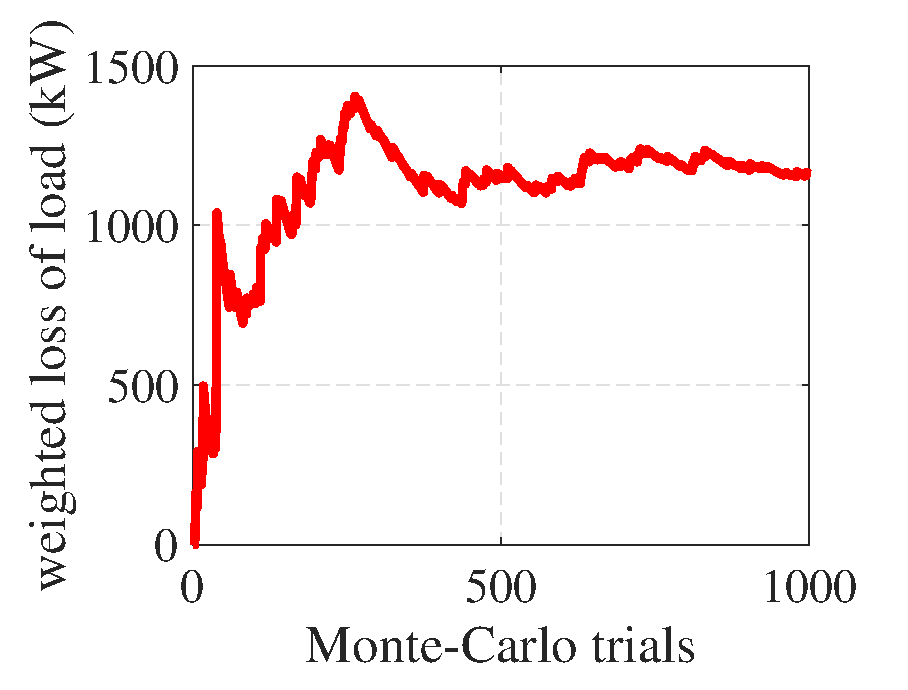
\includegraphics[width=0.42\linewidth]{figures/speed_15_MC_base.eps}
        \label{fig:MCS_1}
    }\hfill
    % \subfigure[]
    {
        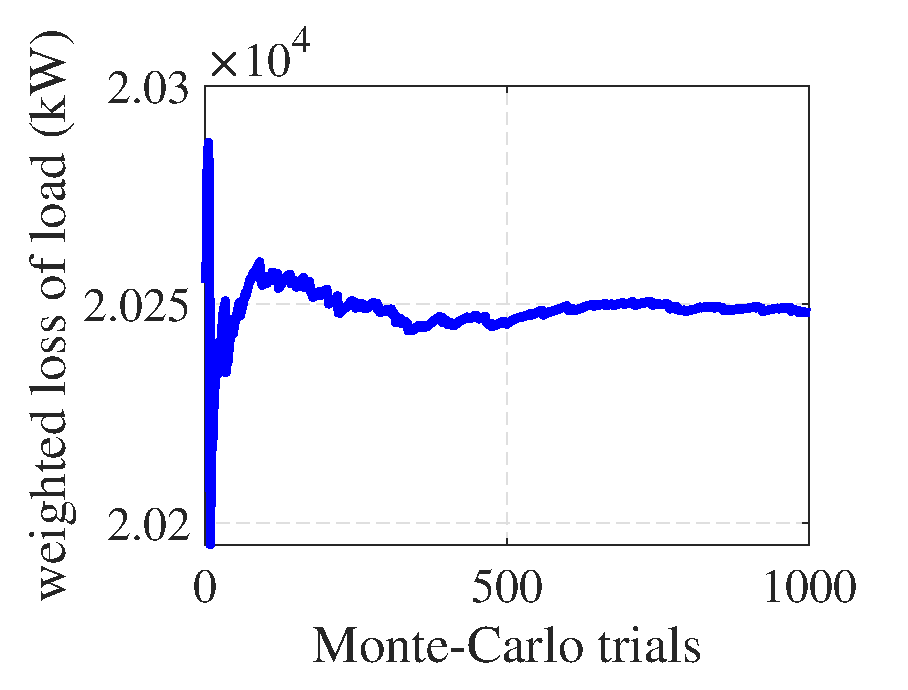
\includegraphics[width=0.42\linewidth]{figures/speed_40_MC_base.eps}
        \label{fig:MCS_2}
     }
     \caption{Moving average of loss of load obtained for 1000 Monte-Carlo trials a) without hardening when $u = 15~m/s$ and $p_f(u) = 0.002$ and b) with line hardening when $u = 40~m/s$ and $p_f(u) = 0.915$. For each wind speed scenario, it can be guaranteed that the prioritized load loss converges after 1000 Monte-Carlo trials.}
     \label{fig:MCS_convergence}
\end{figure}

\begin{figure}[h]
     \centering
    %  \subfigure[]
     {
        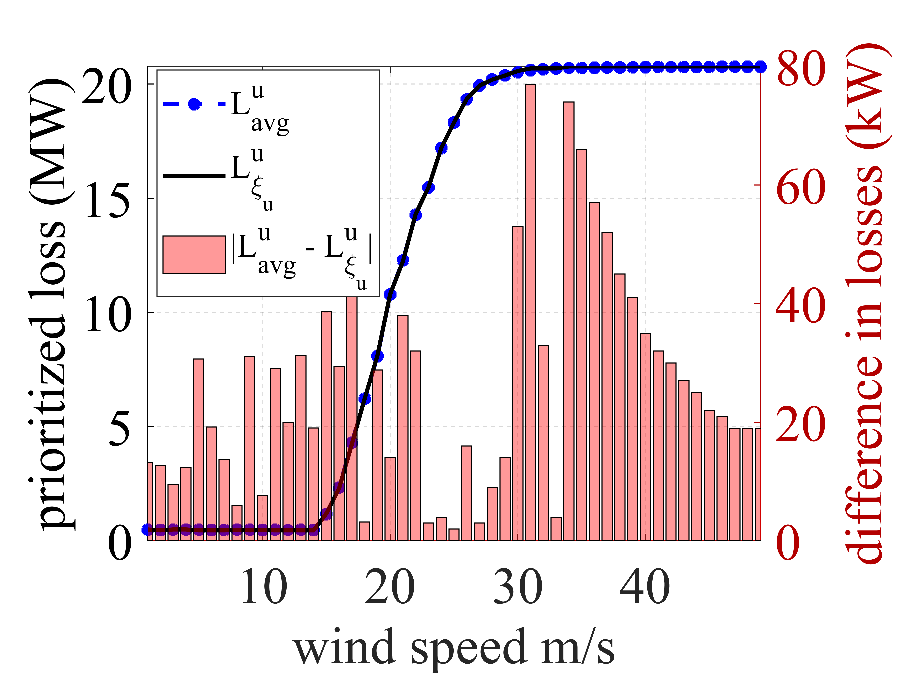
\includegraphics[width=0.42\linewidth]{figures/scenario_new_load_base.eps}
        \label{fig:scen_set_1}
    }\hfill
    % \subfigure[]
    {
        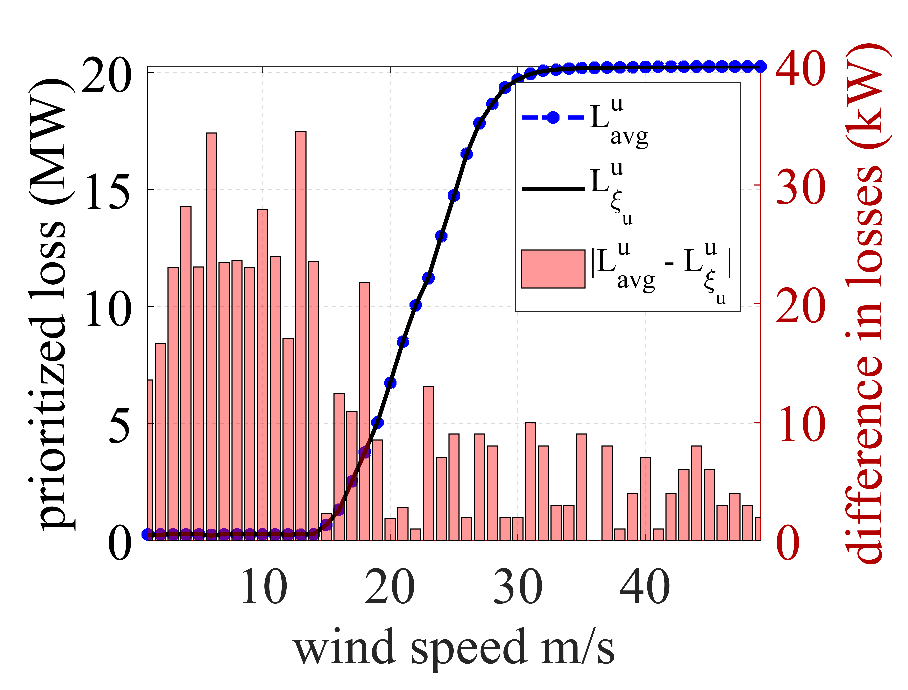
\includegraphics[width=0.42\linewidth]{figures/scenario_new_load_harden.eps}
        \label{fig:scen_set_2}
     }
     \caption{Comparison of prioritized load loss obtained for two sets of reduced scenarios a) without hardening b) with hardening.}
     \label{fig:scenario_reduction}
\end{figure}

\paragraph{Risk-based Planning}
In this long-term planning problem, 6 DG locations are pre-selected as potential locations for the placement of DG units. The selected potential DG locations are nodes 95, 122, 39, 85, 56, and 66. However, the DG locations are decided by the optimization model and $\delta_i^{DG} = 1$ if and only if $\beta_i^{DG} > 0$. From the operator's perspective, it is often practical to have a limited budget while planning the siting and sizing strategies for DGs. The total budget is constrained so that the sum of the DG units is less than or equal to 900 kW.  For risk-driven problems, $\alpha$ is set at 0.95, meaning that 5\% tail scenarios (HILP) are considered to have greater risks.

\begin{table}[t]
    \centering
    \caption{Base case expected value and $CVaR_\alpha$ of prioritized load loss.}
    \begin{tabular}{|c|c|c|c|}
    \hline
          line hardening & $\mathbb{E}(Q(\delta, \mathcal{E}))$ in kW & $CVaR_\alpha(Q(\delta, \mathcal{E}))$ in kW \\
    \hline
         No & 5982.57  & 20601.58  \\
    \hline
         Yes & 4541.76  & 19839.39 \\ 
    \hline
    \end{tabular}
    \label{tab:base_case}
\end{table}

\begin{table}
    \centering
    \caption{Expected value and $CVaR_\alpha$ of prioritized load loss and prioritized critical load (PCL) picked up for different values of $\lambda$. The DG planning strategy differs along with the risk preference defined by $\lambda$. All of the values mentioned here are in kW.}
    \begingroup
    \setlength{\tabcolsep}{5pt} % Default value: 6pt
    \renewcommand{\arraystretch}{1.5}
    \begin{adjustbox}{width=1\textwidth,center=1\textwidth}
    \color{black}{
    \begin{tabular}{|c!{\vrule width 1.5pt}c|c|c!{\vrule width 1.5pt}c|c|c!{\vrule width 1.5pt}c|c|c!{\vrule width 1.5pt}c|c|c!{\vrule width 1.5pt}c|c|c!{\vrule width 1.5pt}c|c|c!{\vrule width 1.5pt}}
    \hline
       \multirow{2}{*}{} & \multicolumn{9}{c!{\vrule width 1.5pt}}{\textbf{WITHOUT LINE HARDENING}} & \multicolumn{9}{c!{\vrule width 1.5pt}}{\textbf{WITH LINE HARDENING}} \\
   \hline
        \multirow{2}{*}{} & \multicolumn{3}{c!{\vrule width 1.5pt}}{\makecell{Existing methods\\~\cite{8329529, 2021IASTATE, 9136725}}} & \multicolumn{6}{c!{\vrule width 1.5pt}}{Proposed method} & \multicolumn{3}{c!{\vrule width 1.5pt}}{\makecell{Existing methods\\~\cite{8329529, 2021IASTATE, 9136725}}} & \multicolumn{6}{c!{\vrule width 1.5pt}}{Proposed method} \\
    
    \cline{2-19}
           & \multicolumn{3}{c!{\vrule width 1.5pt}}{$\bm{\lambda = 0}$} & \multicolumn{3}{c!{\vrule width 1.5pt}}{$\bm{\lambda = 0.5}$} & \multicolumn{3}{c!{\vrule width 1.5pt}}{$\bm{\lambda = 1}$}& \multicolumn{3}{c!{\vrule width 1.5pt}}{$\bm{\lambda = 0}$} & \multicolumn{3}{c!{\vrule width 1.5pt}}{$\bm{\lambda = 0.5}$} & \multicolumn{3}{c!{\vrule width 1.5pt}}{$\bm{\lambda = 1}$} \\
    \hline
         $\mathbb{E}(Q(\delta,\mathcal{E}))$ & \multicolumn{3}{c!{\vrule width 1.5pt}}{3567.12} & \multicolumn{3}{c!{\vrule width 1.5pt}}{3586.28} & \multicolumn{3}{c!{\vrule width 1.5pt}}{3595.51} & \multicolumn{3}{c!{\vrule width 1.5pt}}{2467.46} & \multicolumn{3}{c!{\vrule width 1.5pt}}{2463.95} & \multicolumn{3}{c!{\vrule width 1.5pt}}{2490.09} \\ 
    \hline
        $CVaR_{\alpha}(Q(\delta,\mathcal{E}))$ & \multicolumn{3}{c!{\vrule width 1.5pt}}{19093.89} & \multicolumn{3}{c!{\vrule width 1.5pt}}{18885.92} & \multicolumn{3}{c!{\vrule width 1.5pt}}{18885.92} & \multicolumn{3}{c!{\vrule width 1.5pt}}{18415.04} & \multicolumn{3}{c!{\vrule width 1.5pt}}{18160.18} & \multicolumn{3}{c!{\vrule width 1.5pt}}{18119.1} \\
    \hline
         \makecell{Expectation of PCL\\ picked up} & \multicolumn{3}{c!{\vrule width 1.5pt}}{15043.93} & \multicolumn{3}{c!{\vrule width 1.5pt}}{15016.64} & \multicolumn{3}{c!{\vrule width 1.5pt}}{15006.62} & \multicolumn{3}{c!{\vrule width 1.5pt}}{16065.76} & \multicolumn{3}{c!{\vrule width 1.5pt}}{16048.17} & \multicolumn{3}{c!{\vrule width 1.5pt}}{16026.12} \\ 
    \hline
        \makecell{$CVaR_{\alpha}$ of PCL\\ picked up} & \multicolumn{3}{c!{\vrule width 1.5pt}}{3406.59} & \multicolumn{3}{c!{\vrule width 1.5pt}}{3603.06} & \multicolumn{3}{c!{\vrule width 1.5pt}}{3603.06} & \multicolumn{3}{c!{\vrule width 1.5pt}}{4953.65} & \multicolumn{3}{c!{\vrule width 1.5pt}}{5580.72} & \multicolumn{3}{c!{\vrule width 1.5pt}}{6295.33}  \\
    \hline
        \multirow{4}{*}{\makecell{DG planning \\strategies}} & $\bm{\beta^{DG}_{39}}$ & $\bm{\beta^{DG}_{56}}$ & $\bm{\beta^{DG}_{66}}$ & $\bm{\beta^{DG}_{39}}$ & $\bm{\beta^{DG}_{56}}$ & $\bm{\beta^{DG}_{66}}$ & $\bm{\beta^{DG}_{39}}$ & $\bm{\beta^{DG}_{56}}$ & $\bm{\beta^{DG}_{66}}$ & $\bm{\beta^{DG}_{39}}$ & $\bm{\beta^{DG}_{56}}$ & $\bm{\beta^{DG}_{66}}$ & $\bm{\beta^{DG}_{39}}$ & $\bm{\beta^{DG}_{56}}$ & $\bm{\beta^{DG}_{66}}$ & $\bm{\beta^{DG}_{39}}$ & $\bm{\beta^{DG}_{56}}$ & $\bm{\beta^{DG}_{66}}$   \\   
        \cline{2-19}
        & 0 & 20 & 370 & 20 & 20 & 340 & 20 & 20 & 370 & 0 & 350 & 330 & 20 & 220 & 255 & 20 & 170 & 330 \\
    \cline{2-19}
        & $\bm{\beta^{DG}_{85}}$ & $\bm{\beta^{DG}_{95}}$ & $\bm{\beta^{DG}_{122}}$ & $\bm{\beta^{DG}_{85}}$ & $\bm{\beta^{DG}_{95}}$ & $\bm{\beta^{DG}_{122}}$ & $\bm{\beta^{DG}_{85}}$ & $\bm{\beta^{DG}_{95}}$ & $\bm{\beta^{DG}_{122}}$ & $\bm{\beta^{DG}_{85}}$ & $\bm{\beta^{DG}_{95}}$ & $\bm{\beta^{DG}_{122}}$ & $\bm{\beta^{DG}_{85}}$ & $\bm{\beta^{DG}_{95}}$ & $\bm{\beta^{DG}_{122}}$ & $\bm{\beta^{DG}_{85}}$ & $\bm{\beta^{DG}_{95}}$ & $\bm{\beta^{DG}_{122}}$ \\
    \cline{2-19}
        & 390 & 0 & 120 & 100 & 300 & 120 & 100 & 270 & 120 & 100 & 0 & 120 & 100 & 305 & 0 & 100 & 280 & 0 \\
    \hline
    \end{tabular}}
    \end{adjustbox}
    \endgroup
    \label{tab:result_first_case}
\end{table}

To identify the trade-off among different DG-based planning strategies, 6 locations --- 39, 56, 66, 85, 95, and 122 --- are selected as potential DG locations. First, we discuss the results for the risk-neutral case ($\lambda=0$). The existing resilience-based planning methods,~\cite{8329529, 2021IASTATE, 9136725}, are focused on the risk-neutral case and used as a comparison for this work. The overall capacity of each of the DGs is shown in Table~\ref{tab:result_first_case}. For risk-neutral planning without line hardening measures, no DGs are required to be placed on nodes 36 and 95. However, for mean-risk and risk-averse situations, the planning strategies change significantly. For risk-involved strategies, it is required to place DGs on nodes 39 and 95 while reducing the DG sizes for the rest of the nodes as shown in Table~\ref{tab:result_first_case}. Hence, the trade-off of including risk minimization in the objective is to increase the number of DG units in the system. This can be fruitful for extreme event scenarios when picking up some of the CLs is required, even though it increases the expected value of prioritized load loss. Table~\ref{tab:result_first_case} also shows the expected value and $CVaR_\alpha$ of prioritized CLs picked up by different planning strategies. It can be seen that the expected value of prioritized CLs picked up does not change much regardless of the risk preference. However, for risk-based strategies (both mean risk and risk-averse), $CVaR_\alpha$ of prioritized CLs picked up increases by $200~kW$ compared to the risk-neutral case. 

The effect of risk aversion is even more pronounced in the case with the line-hardening strategy. Fig.~\ref{fig:neutral_vs_averse_harden} shows a restoration and planning solution for a specific scenario of HILP nature, $u = 28~m/s$. The lines and nodes with black color are the energized section, whereas non-energized sections are represented by gray. Similarly, red lines represent out-of-service lines due to the particular outage scenario.
Similar to the restoration for cases without line hardening measures, the risk-neutral solution does not include DGs in nodes 39 and 95. When the objective is risk-neutral ($\lambda=0$) some of the prioritized critical loads are not picked up in this specific scenario as picking up critical loads in this scenario would not affect the expected value of load served for the overall scenarios. Since the objective is to minimize the expected value of prioritized load loss for entire scenarios, DG at location 95 is not selected. Note that the probability of HILP scenarios is low. Since the expected value contains the product of this probability with the objective function in the restoration phase, the net value is significantly low to affect the overall expected value. However, when the objective is risk-averse, any prioritized load that the nearest possible DG can pick up is given the top priority for any HILP event. For instance, it can be seen that load at node 62 is picked up by DG at node 95 through path 95-93-94-54-57-60-62.
Hence, this draws an important conclusion that risk-averse decisions enhance long-term resilience planning by focusing the extreme HILP events. Contrary to the existing methods in~\cite{8329529, 2021IASTATE, 9136725}, the prioritized CLs have a high chance of being picked up when an HILP event is realized by including risk minimization in the objective. However, when attempting to minimize the risk-averse objective (i.e., the $CVaR_\alpha$), we incur an additional DG cost in the overall planning budget to meet the requirements for risk-averse planning. Thus, through the proposed approach and by including $CVaR_\alpha$ minimization in the objective function, prioritized critical loads can be properly restored in case of HILP events. Furthermore, with the changing trade-off between the expectation and the $CVaR_\alpha$ of the prioritized load loss, the expected value \textit{generally} decreases with the increase in $\lambda$. 

\begin{figure}[ht]
        \centering
        % \subfigure[]
        {
        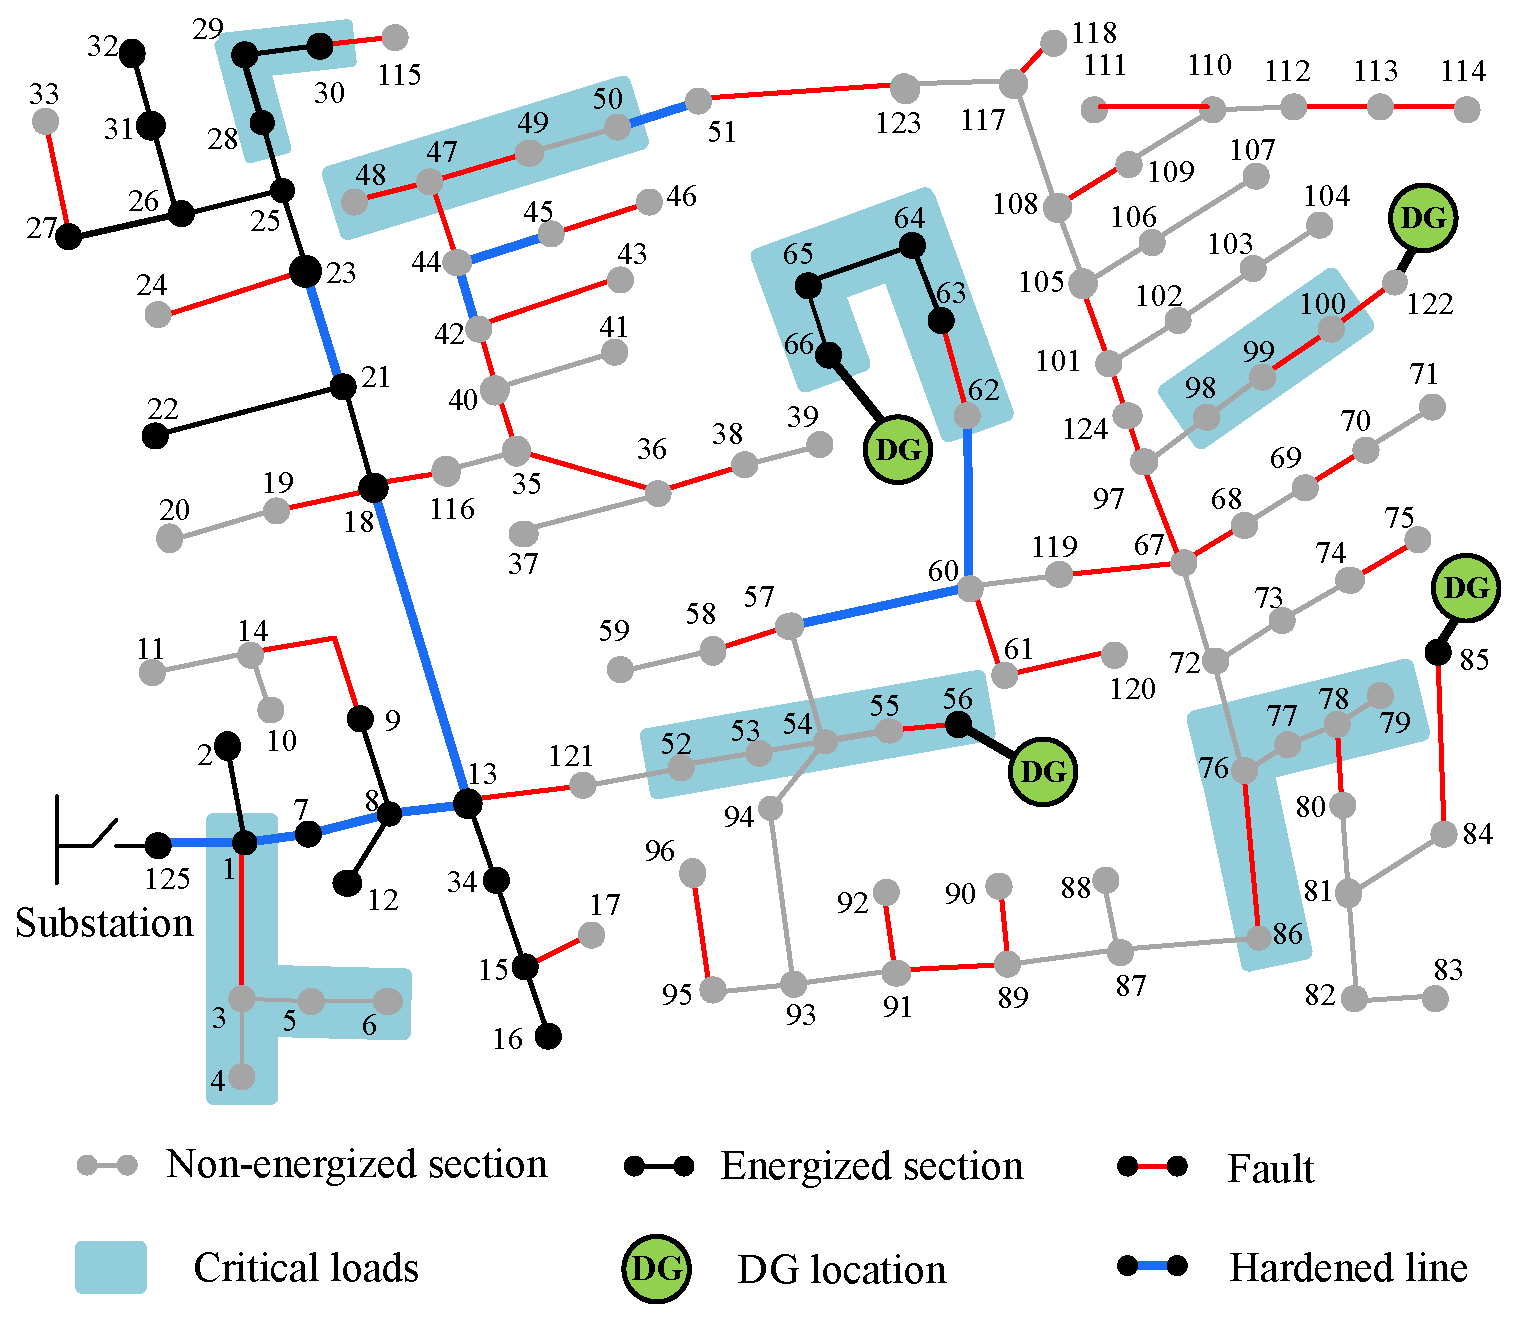
\includegraphics[width=0.48\textwidth]{figures/harden_neutral.eps}
    }\hfill
    % \subfigure[]
    {
        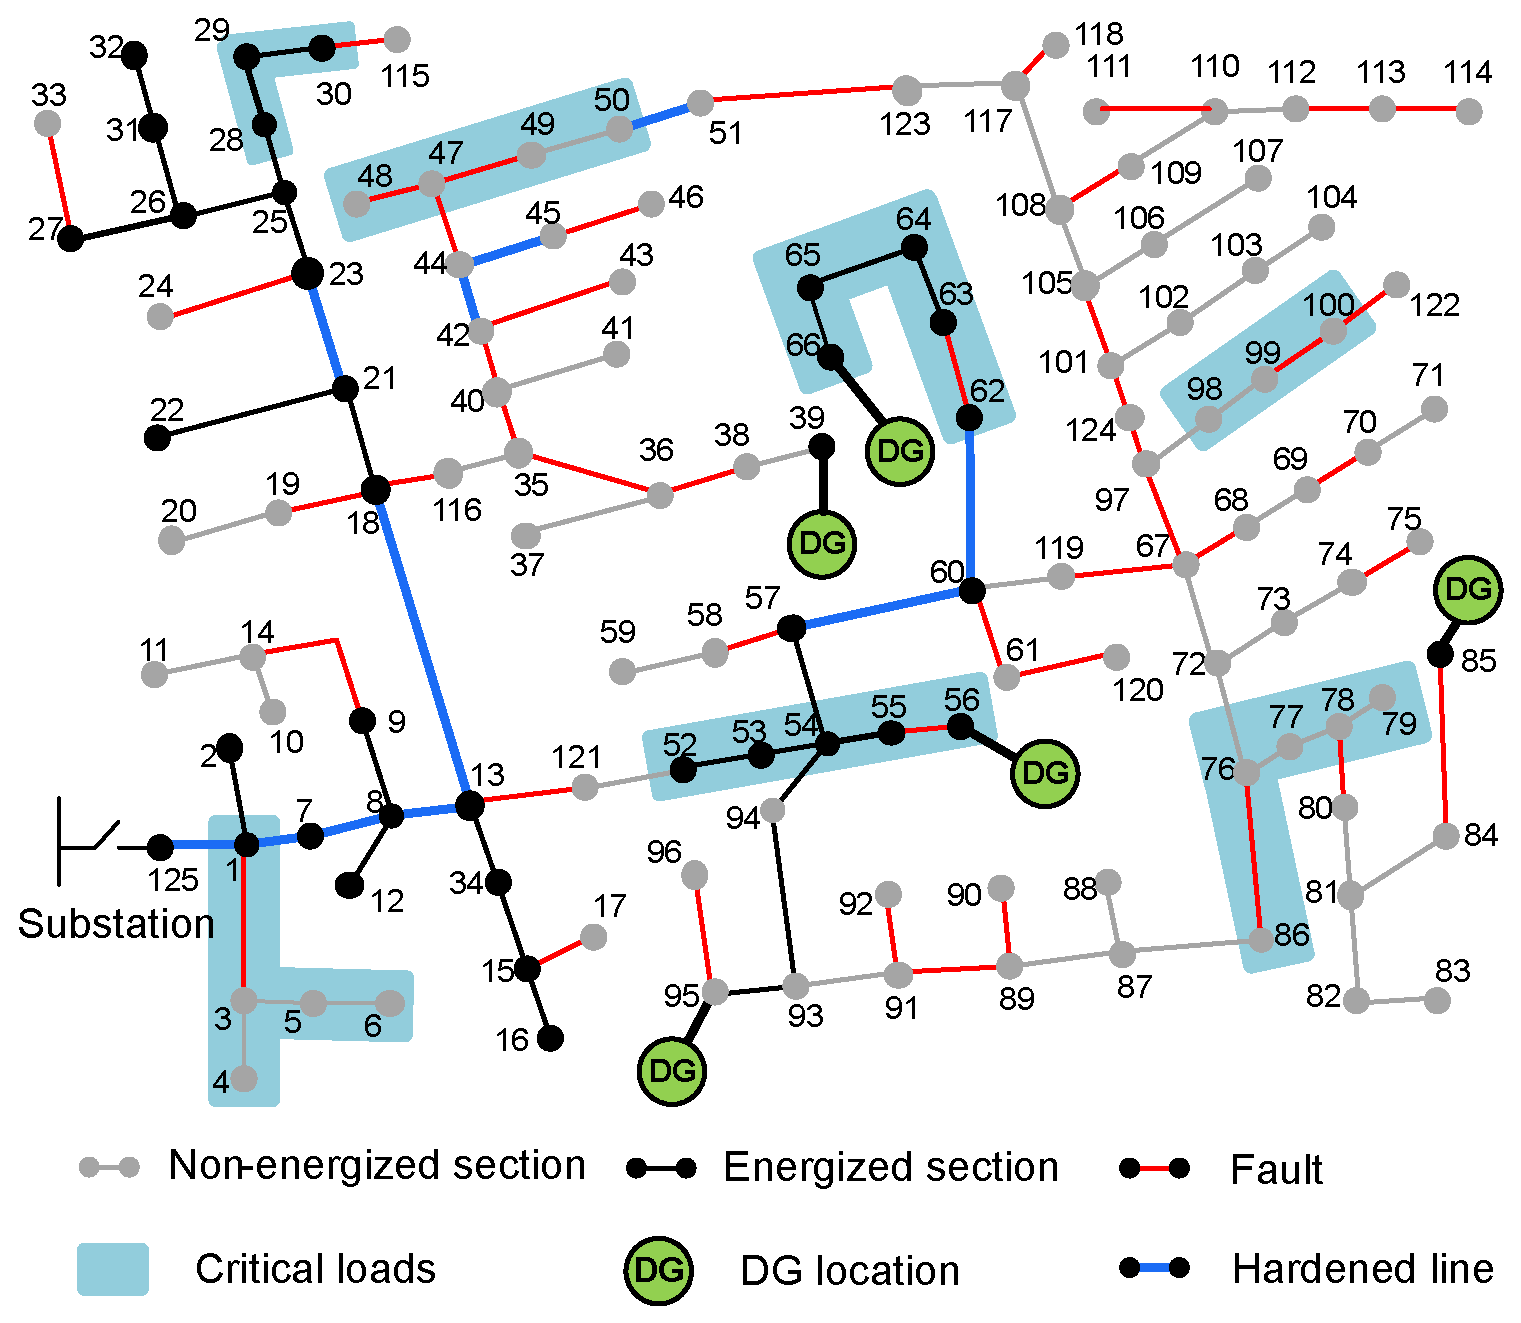
\includegraphics[width=0.48\textwidth]{figures/harden_averse.eps}  
     }
    \caption{\revise{DG sizing and siting solution for a specific scenario with additional hardening measures for a) risk-neutral and b) risk-averse planning strategy.}}
    \label{fig:neutral_vs_averse_harden}
\end{figure}

\paragraph{Sensitivity Analysis}
The value of $CVaR$ depends on several factors such as investment decisions, budget, risk preference, and scenarios under consideration. Here, we present a few of the sensitivity analyses and discuss their impacts on $CVaR$. For simplicity, the analyses are performed only on the system with additional hardening measures already in place and for sensitivity based on time complexity, the analysis is done in terms of expected value of the second stage.

\begin{figure}[t]
    \centering
    \includegraphics[width=0.8\textwidth]{figures/CVaR_alpha_harden.eps}
    \vspace{-0.6cm}
    \caption{Comparison of $CVaR_\alpha$ of prioritized loss of load for different values of $\alpha$ and risk preference.}
    \label{fig:CVaR_vs_alpha}
\end{figure}

\begin{figure}[!ht]
     \centering
    %  \subfigure[]
     {
        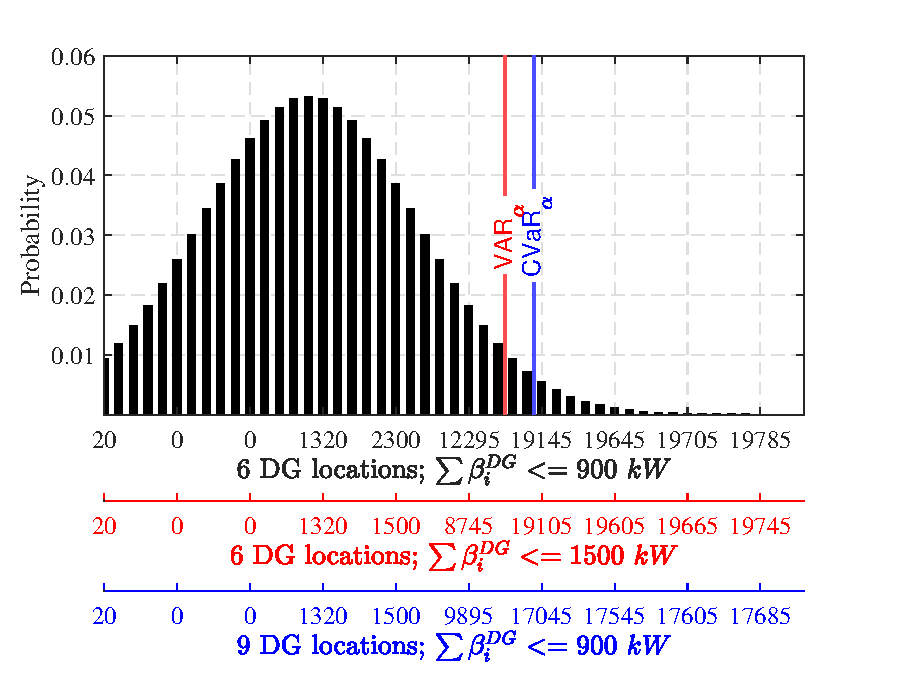
\includegraphics[width=0.7\textwidth]{figures/DG_tradeoff_neutral.eps}
        \label{fig:DG_neutral}
    }
    % \subfigure[]
    {
        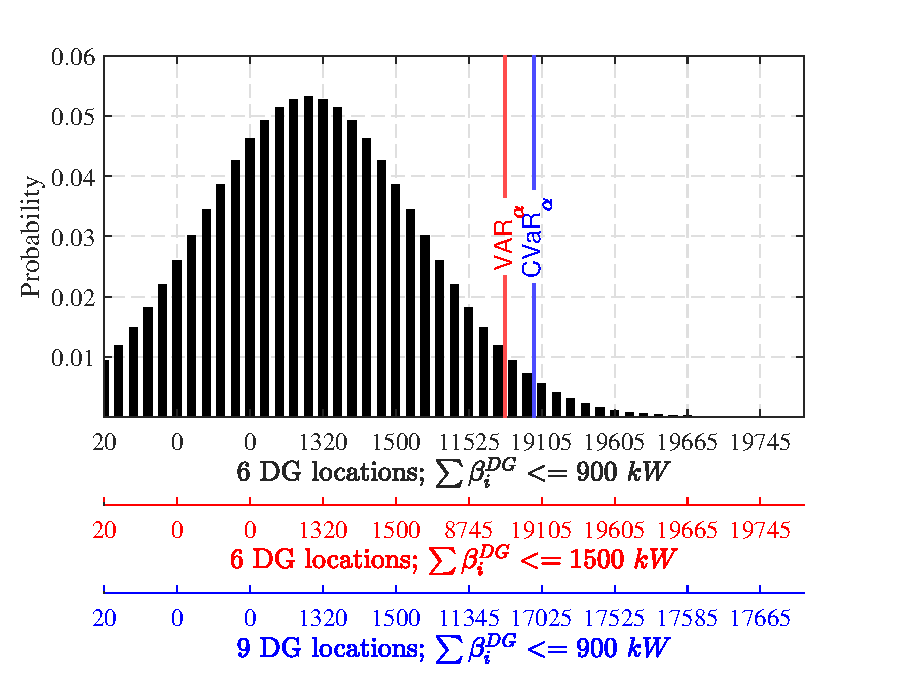
\includegraphics[trim ={0 0 0 0.5cm} ,clip, width=0.7\textwidth]{figures/DG_tradeoff_averse.eps}
        \label{fig:DG_averse}
     }
     \caption{$CVaR_\alpha$ for different DG investment strategies for a) risk-neutral and b) risk-averse planning. The value on the x-axis represents the prioritized loss of load for each $\xi$ with corresponding $p_\xi$ represented on the y-axis.}
     \label{fig:DG_tradeoffs}
     \vspace{-0.4cm}
\end{figure}

\begin{figure*}[!t]
        \centering
        % \vspace{0.5 cm}
        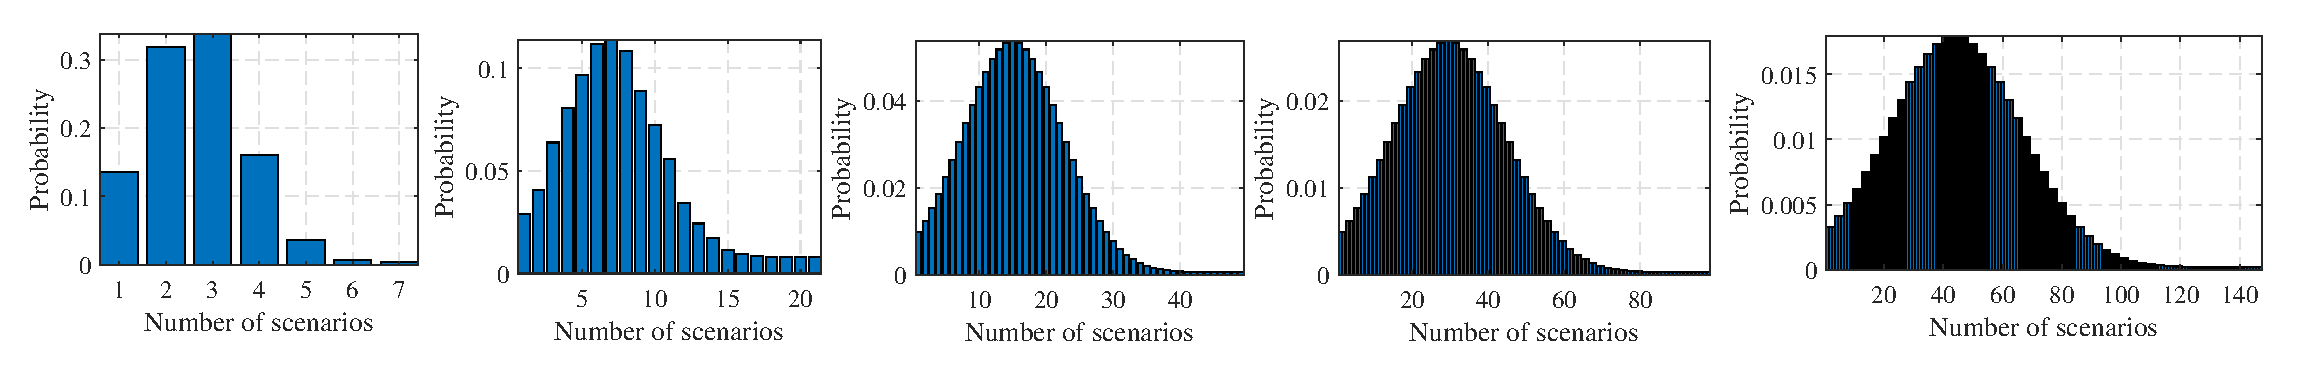
\includegraphics[width=\textwidth]{figures/different_scenarios_2.eps}
        \caption{\revise{Different number of scenarios with respective probabilities of occurrence: (a) 7 scenarios, (b) 21 scenarios; (c) 49 scenarios, (d) 98 scenarios e) 147 scenarios.}}
        \label{fig:scen_probab}
\end{figure*}

\paragraph{Change in confidence level}
The risk parameters $\alpha$ and $\lambda$ can affect the planning decisions. The value of $CVaR_\alpha$ highly depends on $\alpha$ as it defines the number of scenarios to be considered in defining the risk. In other words, $\alpha$ can also be defined as risk percentage. For a higher value of $\alpha$, the value of $VAR_\alpha$ increases, and hence, $CVaR_\alpha$ represents the scenarios that create greater losses in the system. Similarly, for a smaller $\alpha$, $CVaR_\alpha$ incorporates a larger number of scenarios with lower losses in risk quantification. Furthermore, as discussed above, an increasing value of $\lambda$ denotes an increase in risk aversion towards planning decisions. Fig.~\ref{fig:CVaR_vs_alpha} shows the relation of $CVaR_\alpha$ for the prioritized loss of load for different values of $\lambda$ and $\alpha$. As discussed, $CVaR_\alpha$ decreases when more scenarios are considered as risky (characterized by $\alpha$). Furthermore, for a fixed $\alpha$, $CVaR_\alpha$ decreases with the increase in the value of $\lambda$ as more importance are given to risk minimization. Appropriate values for $\alpha$ and $\lambda$ need to be selected based on planners' risk aversion criteria.

\paragraph{Change in investment strategies}
Changing investment strategies and allocating the budget properly can also affect the overall planning cost. First, the overall budget for DG sizing and installation is increased so that $\mathcal{C}^{DG}_{max}$ corresponds to $P_{DG}^{max} = 1500~kW$ for the same set of DGs and their potential locations. Secondly, 3 additional DG locations (47, 27, and 114) are identified as potential DG placement locations. Fig.~\ref{fig:DG_tradeoffs} shows the distribution of prioritized loss of load when different DG planning measures are taken for risk-neutral and risk-averse cases, respectively. It is interesting to notice that increasing the budget to increase the capacity of DGs has a limited effect on the $CVaR_\alpha$ minimization. However, the expected value of prioritized load loss decreases to $2222.43~kW$ from $2467.46~kW$. The conclusion is consistent for the risk-averse case. However, increasing the number of potential DG locations led to significant improvement in $CVaR_\alpha$ minimization. The change in expected loss is, however, insignificant. For the case with 9 potential DG locations, the value of $CVaR_\alpha$ decreases from $18415.04~kW$ to $16385.51~kW$, for the risk-neutral case, and from $18119.1~kW$ to $15811.59~kW$, for the risk-averse case. Thus, with a limited budget, multiple DG sites with smaller DGs are more effective in improving resilience. 

\paragraph{Change in number of scenarios and set of scenarios} 
Fig.~\ref{fig:scen_probab} shows five case studies simulated to evaluate the impacts of the number of scenarios (used in optimization) on solution quality and solve time; (a) 7 scenarios, (b) 21 scenarios, (c) 49 scenarios, (d) 98 scenarios, (e) 147 scenarios.  Hence, for each case, different scenario sets are obtained using the method discussed in Algorithm 1. Fig.~\ref{fig:scen_vs_time} shows the objective function value for the different number of scenarios (used in the optimization problem) along with the corresponding solve times. The result for each case is obtained by taking an average of 10 representative scenario sets closest to the average representative scenario. We can clearly observe the trade-off between the number of scenarios, solution quality, and solve time. When a higher number of scenarios are used in optimization, the solution quality improves; however, it also leads to a significant increase in the solve time. It is also interesting to note that the solution obtained for 49 scenarios (2719.17 kW) is very close to the one obtained for 147 scenarios (2764.16 kW). However, the solve time for the problem with 147 scenarios is 11 times greater than that with 49 scenarios. Hence, 49 scenarios work well from the point of view of solution as well as solve time as the additional number of scenarios increases the computational complexity with no significant improvement in the objective value.

\begin{figure}[!t!]
    \centering
    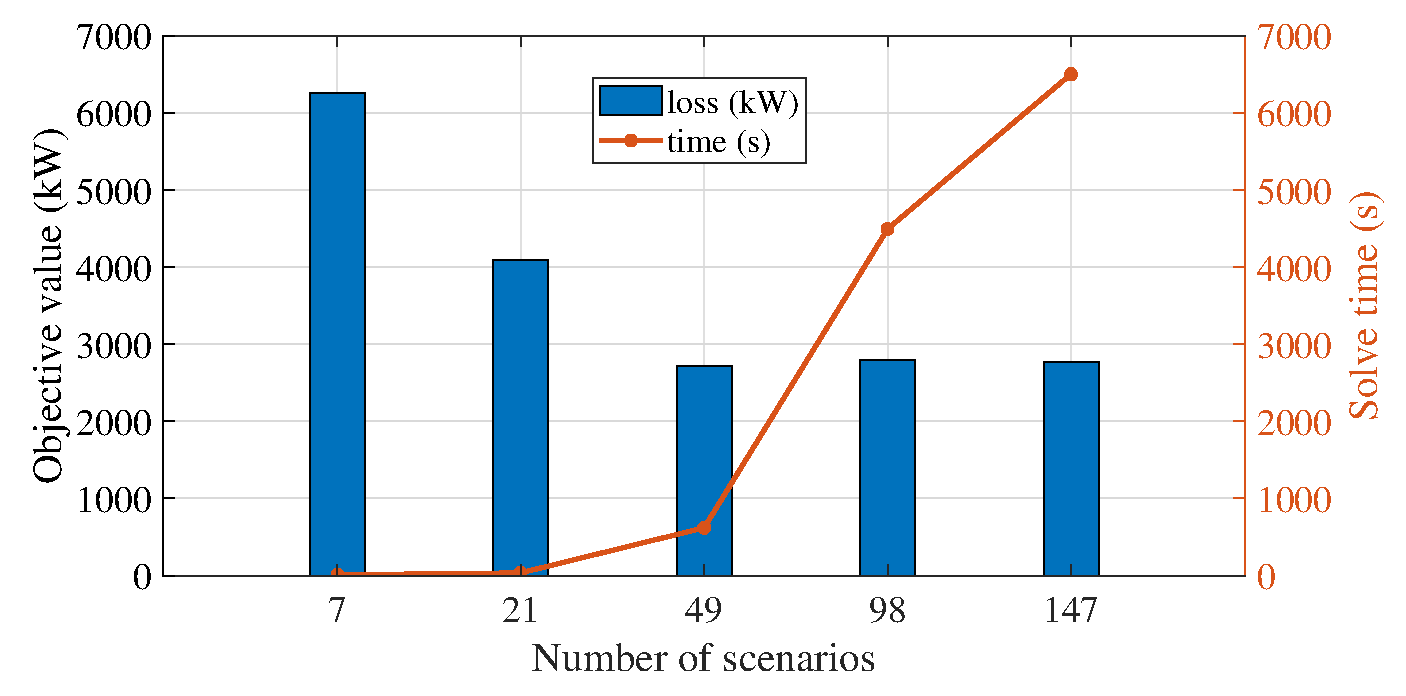
\includegraphics[width=0.7\textwidth]{figures/scenario_vs_time.eps}
    \caption{\revise{Comparison of objective value and solve time for a different number of scenarios.}}
    \label{fig:scen_vs_time}
\end{figure}

\begin{figure}[t]
    \centering
    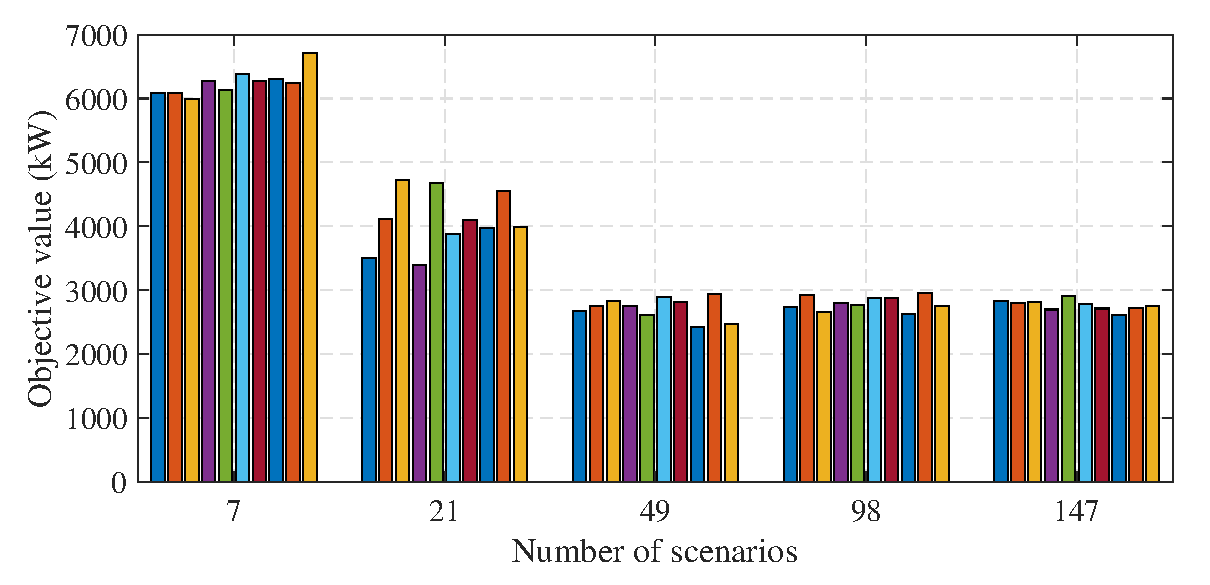
\includegraphics[width=0.7\textwidth]{figures/bundled_scenarios.eps}
    \caption{\revise{Comparison of objective value on a different set of scenarios for each number of scenarios sampled.}}
    \label{fig:scen_sets}
\end{figure}


\clearpage
%%%%%%%%%%%%%%%%%%%%%%%%%%%%%%% Spatiotemporal Impact Assessment Chapter %%%%%%%%%%%%%%%%%%%%%%%%%
\section{Spatiotemporal impact assessment of hurricanes and storm surges in electric power systems}

\begin{table}[h]
    \centering
        \caption{\textcolor{black}{95\% confidence interval of the solution obtained using different scenario sets for each number of scenarios.}}
        {\color{black}
        \begin{tabular}{c|c|c}
        \hline
             \makecell{Number of \\ scenarios} & 95\% CI (kW) & \makecell{Average objective \\ value (kW)} \\
        \hhline{===}
             $7$ & $\left[6105.95, 6393.99\right]$ & $6249.57$ \\
        \hline
            $21$ & $[3764.35, 4414.53]$ & $4089.44$ \\
        \hline
            $49$ & $[2596.13, 2842.21]$ & $2719.17$ \\
        \hline
            $98$ & $[2721.20, 2879.54]$ & $2800.37$ \\
        \hline
            $147$ & $[2705.10, 2823.21]$ & $2764.16$ \\
        \hline
        \end{tabular}}
        \label{tab:95_CI}
    \end{table}

\clearpage
% \newpage
%%%%%%%%%%%%%%%%%%%%%%%%%%%%%%% Spatiotemporal Impact Assessment Chapter %%%%%%%%%%%%%%%%%%%%%%%%%
\section{Spatiotemporal impact assessment of hurricanes and storm surges in electric power systems}
\subsection{Prior work on extreme weather impact assessment on power systems and their limitations}
Several existing works model the impacts of hurricanes on the power grid due to high-speed winds~\cite{7434044}. To model the spatial nature of the event, other works divided the entire power grid into zones such that each zone experiences a different wind speed~\cite{Trakas2018}. However, based on the hurricane's trajectory, each component is impacted differently as the hurricane moves inland, rendering the simplified hurricane model inaccurate for grid impact assessment. Other works model the effect of hurricanes on distribution grid~\cite{nguyen2019assessing}. Since the overall spatial exposure of a hurricane is greater than an entire distribution grid for each time step, the analysis based on the distribution system alone would not be meaningful enough.
Furthermore, none of these works model the impact of storm surges on the power grid. In~\cite{souto2022power}, a power system impact assessment framework is presented to identify potential mitigation strategies and enhance resilience against floods. A stochastic optimization framework for substation hardening against storm surge is presented in~\cite{shukla2021scenario}. \cite{Feng2022} evaluated the impacts of tropical cyclones and heatwaves on the power grid. The existing work, however, lacks the spatiotemporal impacts analysis of hurricanes characterizing the compound effects of high-speed wind and flooding. 

\subsection{Proposed Approach and Modeling}
This work aims to develop a compound spatiotemporal effect of hurricanes and storm surges on electric power systems. First, dynamic hurricane scenarios are generated based on historical hurricane tracks and storm surge scenarios are obtained based on the obtained hurricane parameters closer to the landfall. Next, sequential Monte Carlo simulation (MCS) is performed for probabilistic tracks and flooding scenarios for each time step as the hurricane moves inland. Finally, we quantify the impacts using a spatiotemporal loss metric based on the compound effect of hurricanes and floods.

\subsubsection{Hurricane Wind field Model}
A part of the impact of hurricanes originates from their wind speed. This wind speed is a vector field centered around the hurricane's eye and changes as it moves inland. This wind field can be modeled as an equation with three variables: $v_{max}$, $R_{v_{max}}$, and $R_s$~\cite{javanbakht2014risk, 9917119}. Here, $v_{max}$ measures the maximum sustained wind speed of the hurricane in knots, $R_{v_{max}}$ measures the distance to $v_{max}$ in nautical miles (nmi), and $R_s$ measures the radius of the hurricane from the hurricane's eye, also known as the radius of the outermost closest isobar (roci), in nmi. Fig.~\ref{fig:static_hurricane} demonstrates the relationship between the wind speed and the distance from the hurricane's eye, and the piecewise mathematical function that represents Fig.~\ref{fig:static_hurricane} is shown in (\ref{eq:static_eq}).

\begin{equation} \label{eq:static_eq}
\small
\begin{aligned}
&v(x)= \begin{dcases} K \times v_{max}(1-exp{[-\Psi x]}) & 0 \leq x<R_{v_{max}} \\
v_{max} \exp \left[- \Lambda \left(x-R_{v_{max}}\right)\right] & R_{v_{max}} \leq x \leq R_{s} \\
0 & x>R_{s}\end{dcases} \\
&\Psi=\frac{1}{R_{v_{max}}} \ln \left(\frac{K}{K-1}\right), K>1;
\quad \Lambda = \frac{\ln \beta}{R_{s}-R_{v_{max}}}
\end{aligned}
\end{equation}

\noindent
$K$ is a known hurricane constant, $x$ is the distance from the hurricane eye, and $\beta$ is the factor that the maximum sustained wind speed will decrease at the hurricane’s boundary $(R_s)$. Using this equation, it can be assumed that the hurricane has no effect outside this boundary.

\begin{figure}[t]
    \centering
    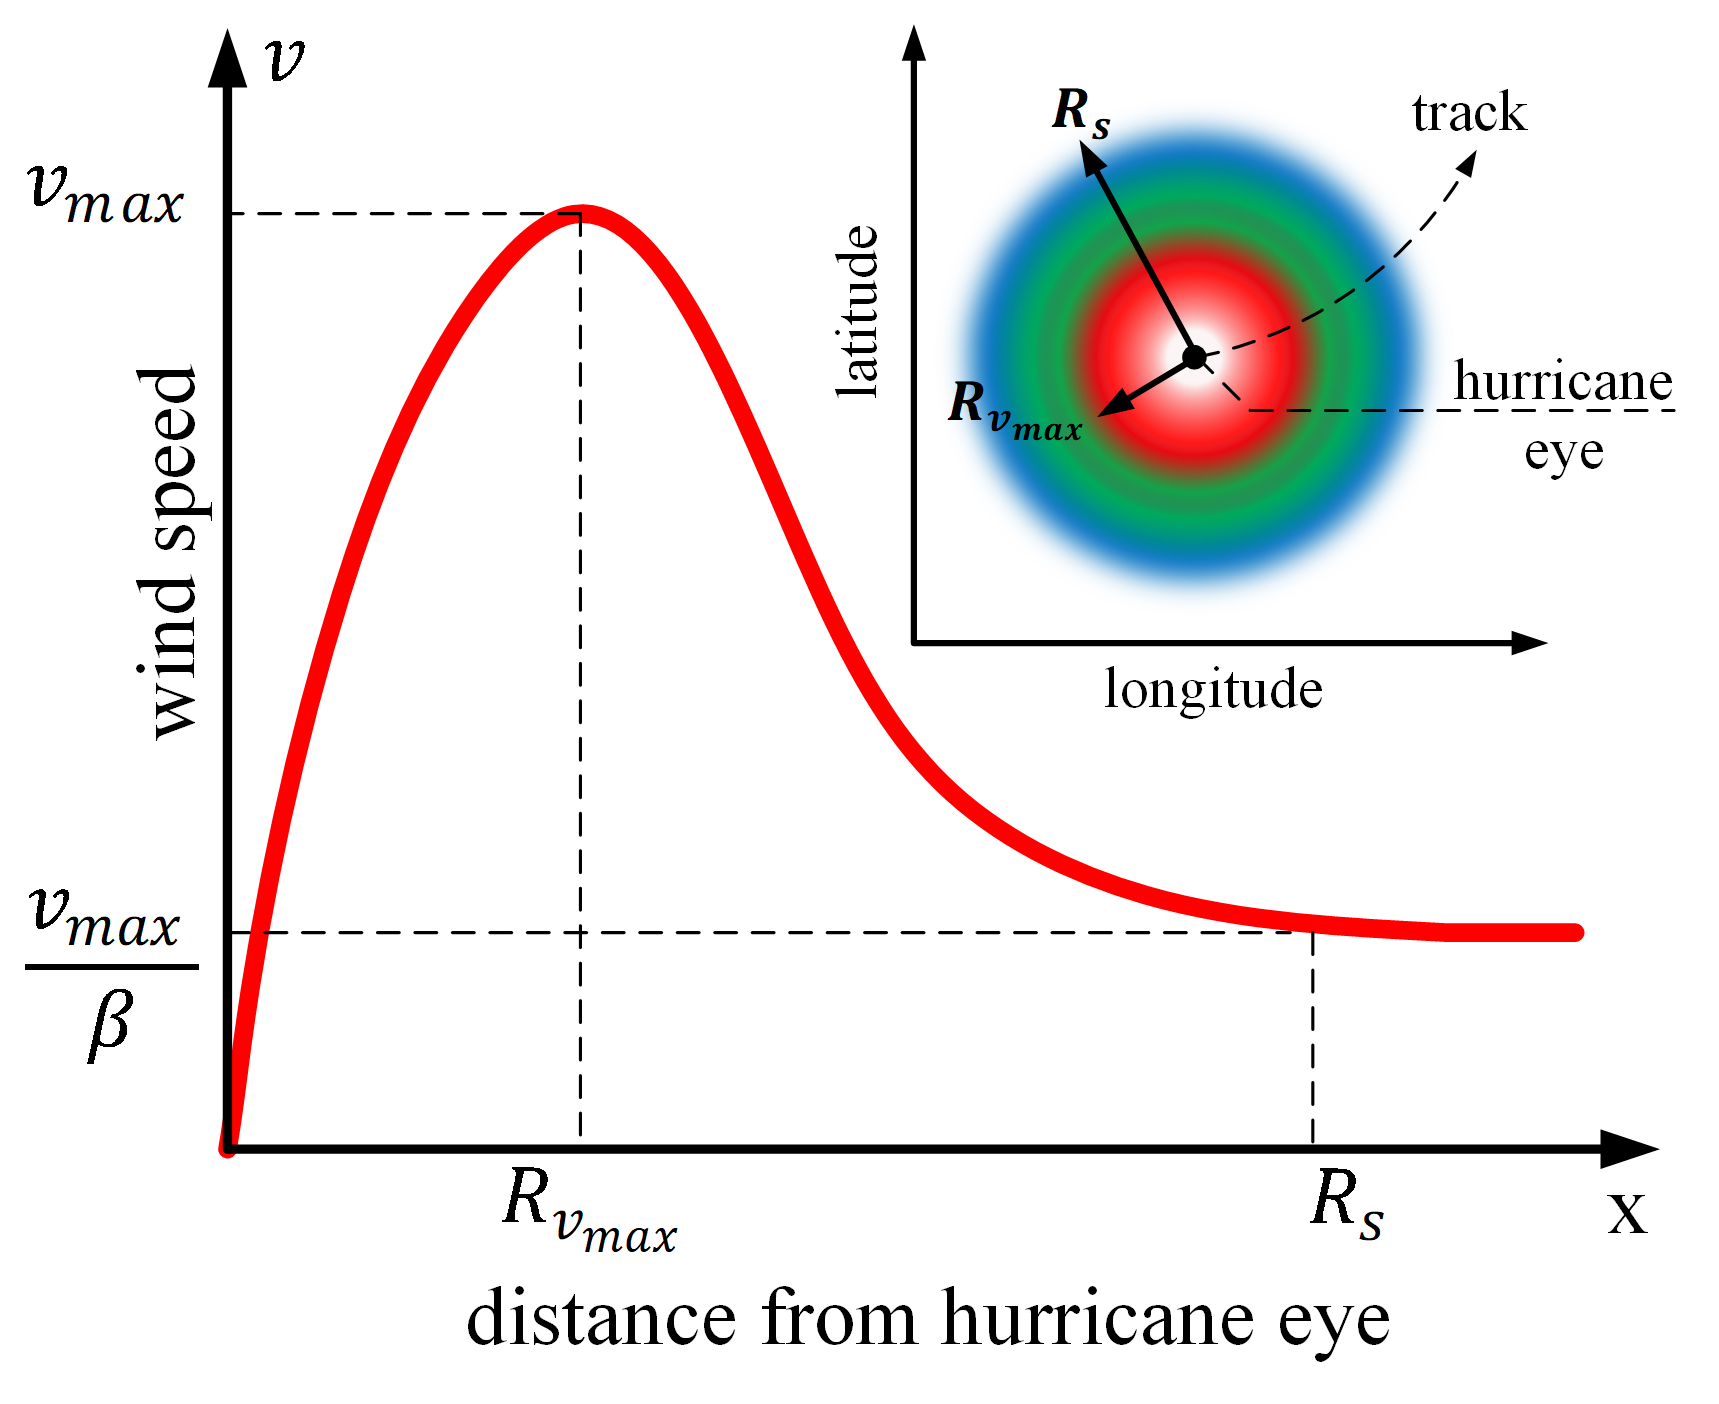
\includegraphics[width=0.55\textwidth]{figures/hurricane_wind_field.png}
    \caption{Static gradient wind field of a typical hurricane.}
    \label{fig:static_hurricane}
\end{figure}

To ensure a realistic hurricane wind field, the wind parameters in (\ref{eq:static_eq}) are obtained using the International Best Track Archive for Climate Stewardship (IBTrACS). IBTrACS is a global collection of tropical cyclones that merges data from multiple agencies to create a database for historical hurricane parameters at various time steps~\cite{Knapp2010}. The hurricane wind field is generated for each time step $t$ by obtaining $\{R_{v_{max}}^t$, $R_{s}^t$, $v_{max}^t\}$ from IBTrACS and using Eq. (\ref{eq:static_eq}). The problem of missing data is often possible when using historical data of higher resolution. IBTrACS, however, has approximated values of wind speed at each specified time interval. The work in~\cite{javanbakht2014risk} argues that the individual elements in $\{R_{v_{max}}^t$, $R_{s}^t$, $v_{max}^t\}$ are highly uncorrelated and hence one can randomly sample the corresponding element to approximate the behavior of the hurricane at that particular instance. Hence, for such situations, we have randomly sampled one of the parameters whenever required. The distribution of three of these parameters for historical hurricanes from 1851 -- 2012 is shown in Fig.~\ref{fig:three graphs}.       

\begin{figure}[ht]
    \centering
    \begin{subfigure}[t]{0.55\textwidth}
        \centering
        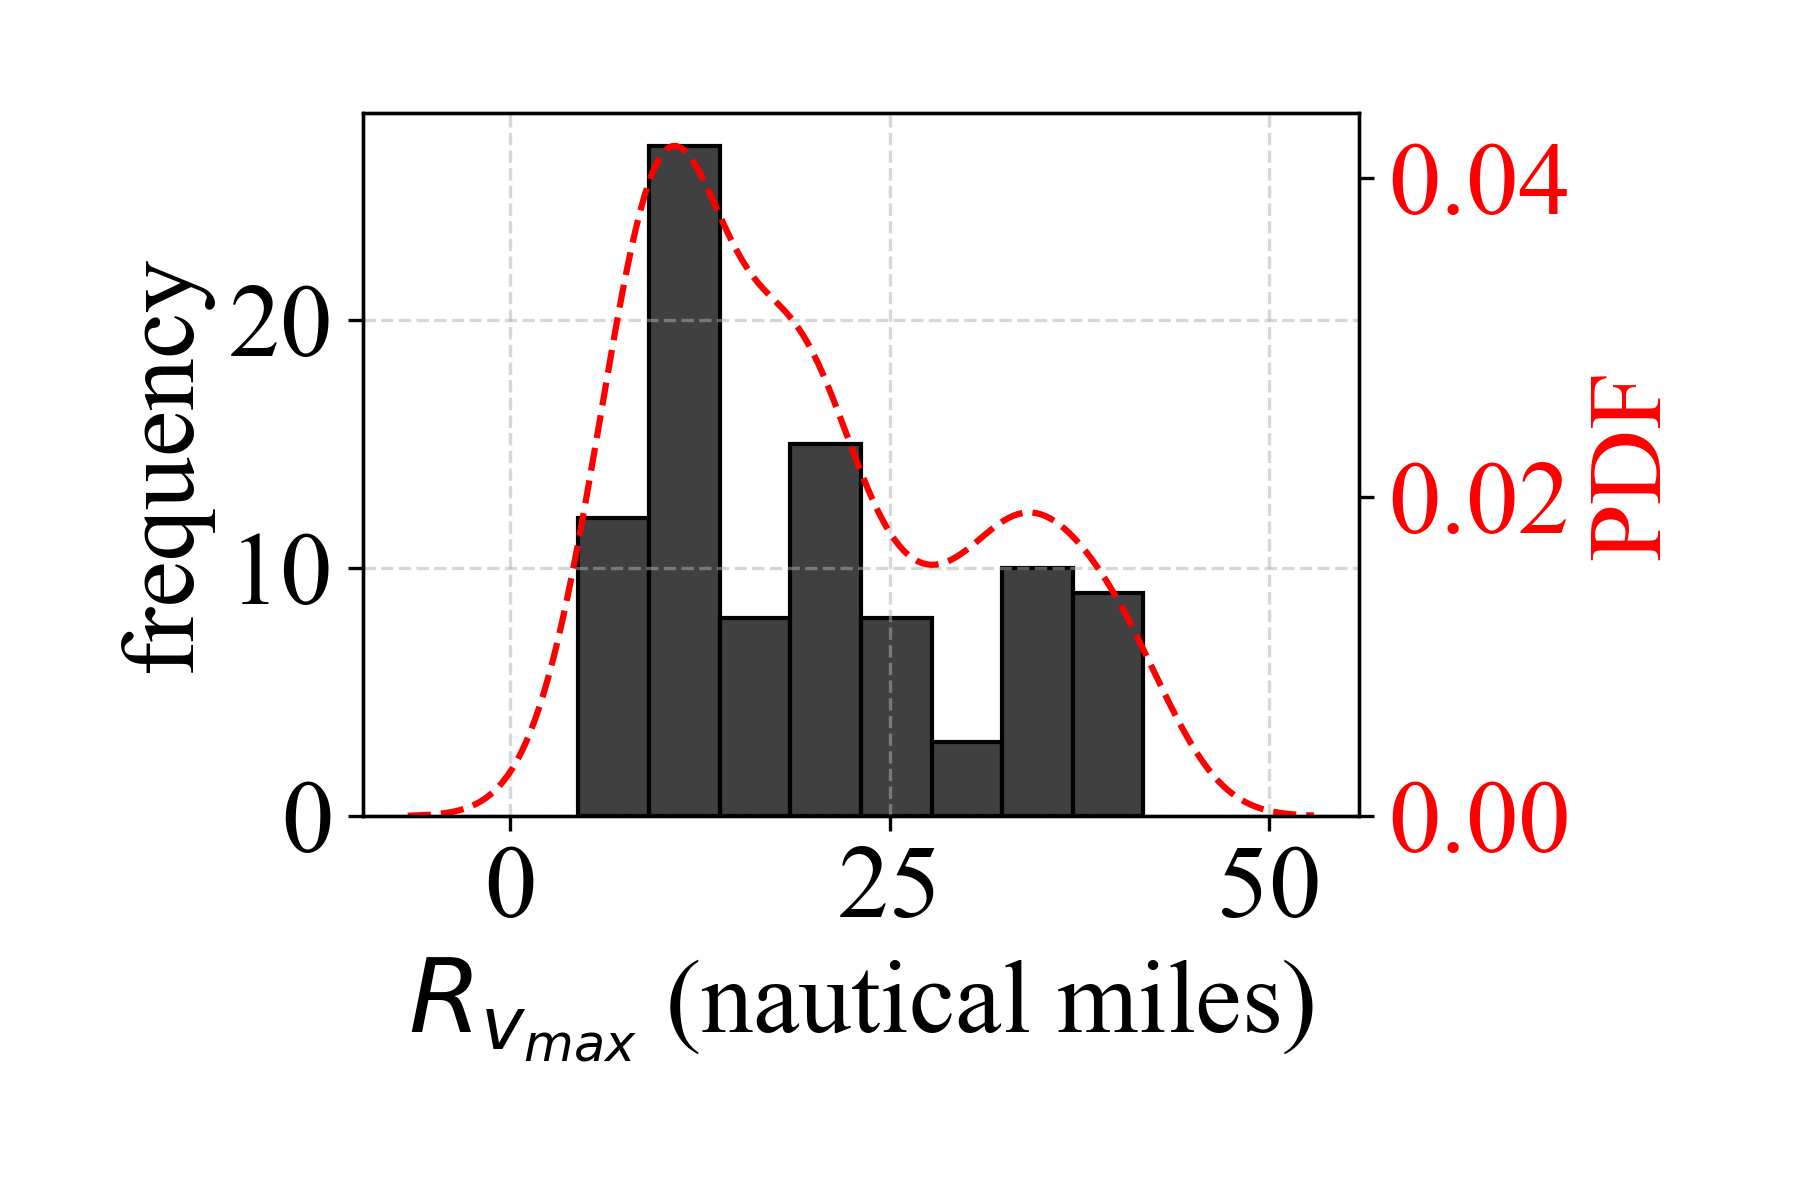
\includegraphics[clip, trim=0cm 0.7cm 0.1cm 0.5cm, width=\linewidth]{figures/Rmw_kde.png}
        \caption{}
        % \label{fig:MC_trial}
    \end{subfigure}%
    \hspace*{\fill}
    \begin{subfigure}[t]{0.55\textwidth}
        \centering
        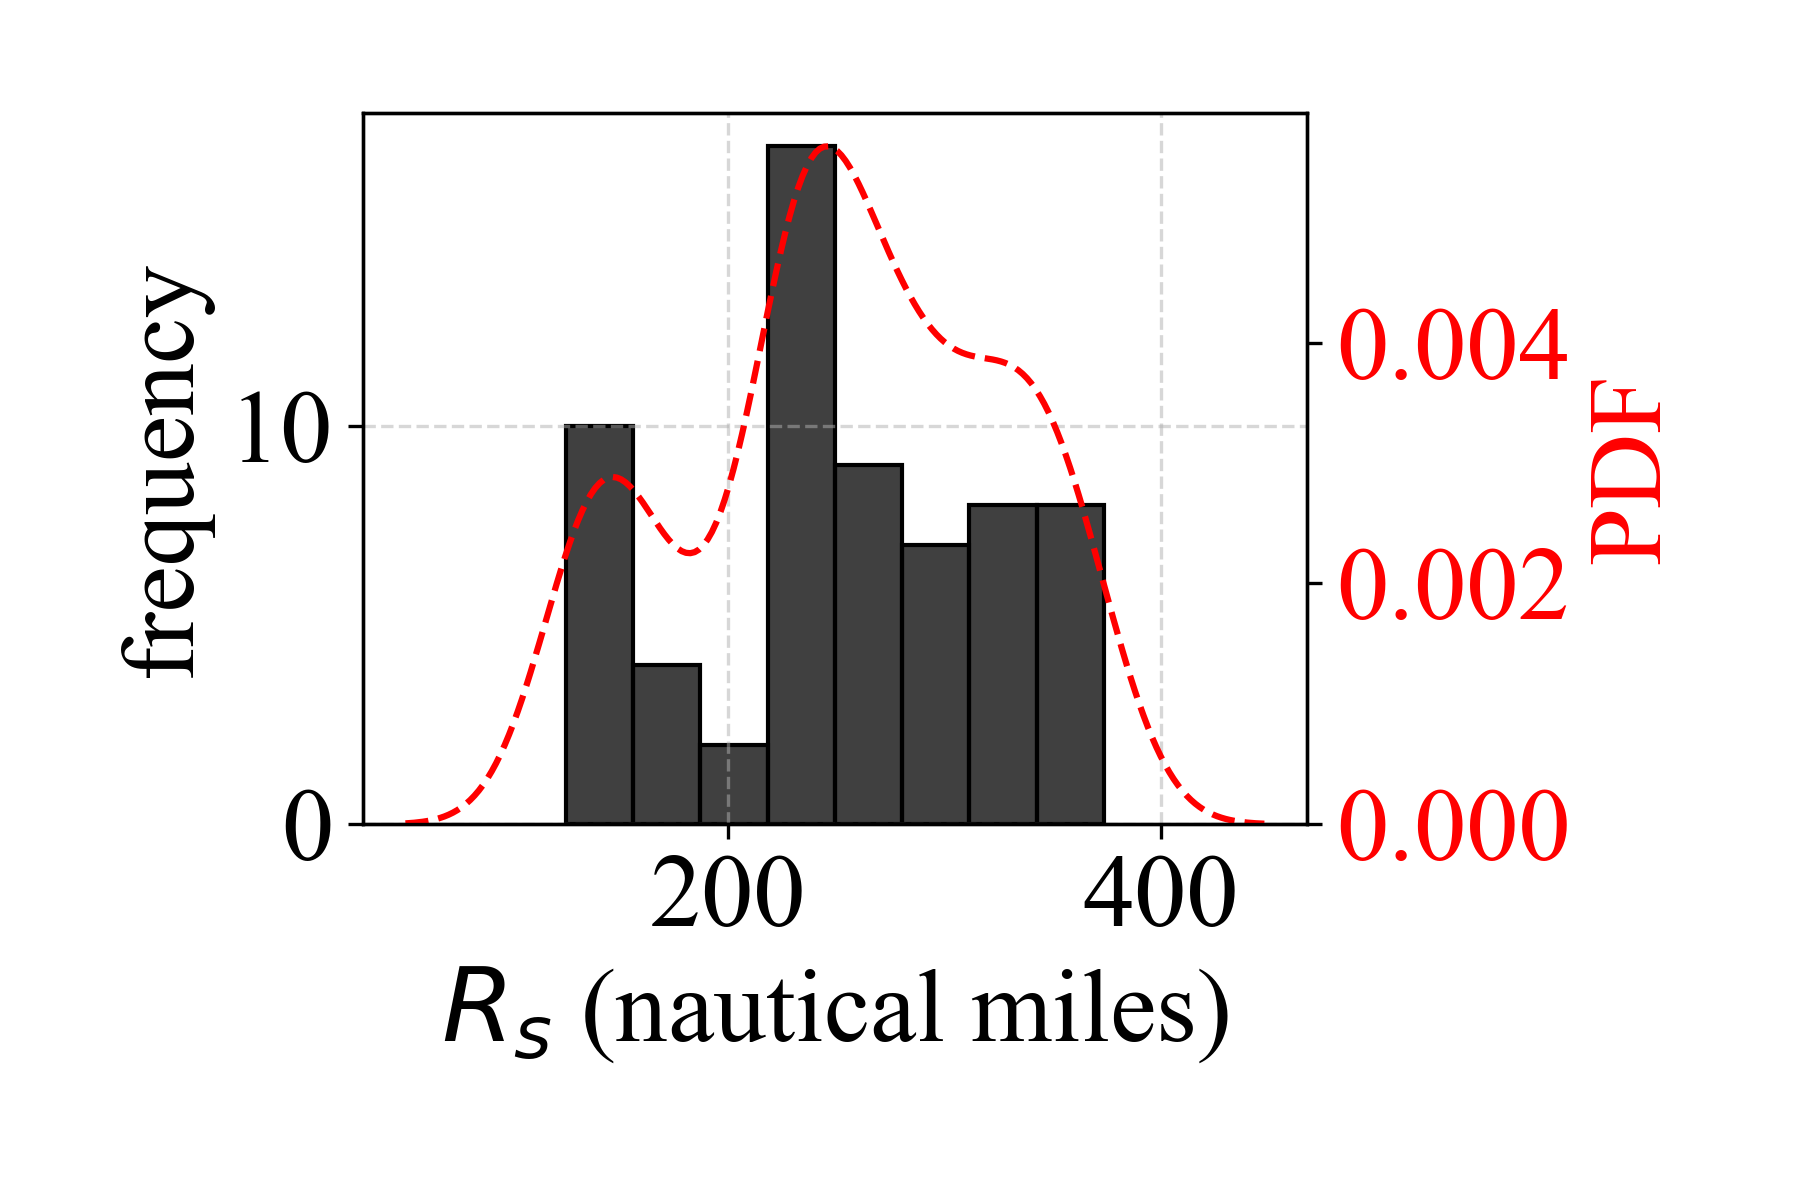
\includegraphics[clip, trim=0cm 0.7cm 0.1cm 0.5cm,width=\linewidth]{figures/Rs_kde.png}
        \caption{}
        % \label{fig:outage_prob}
    \end{subfigure}
    \bigskip
    \hspace*{\fill}
    \begin{subfigure}[t]{0.55\textwidth}
        \centering
        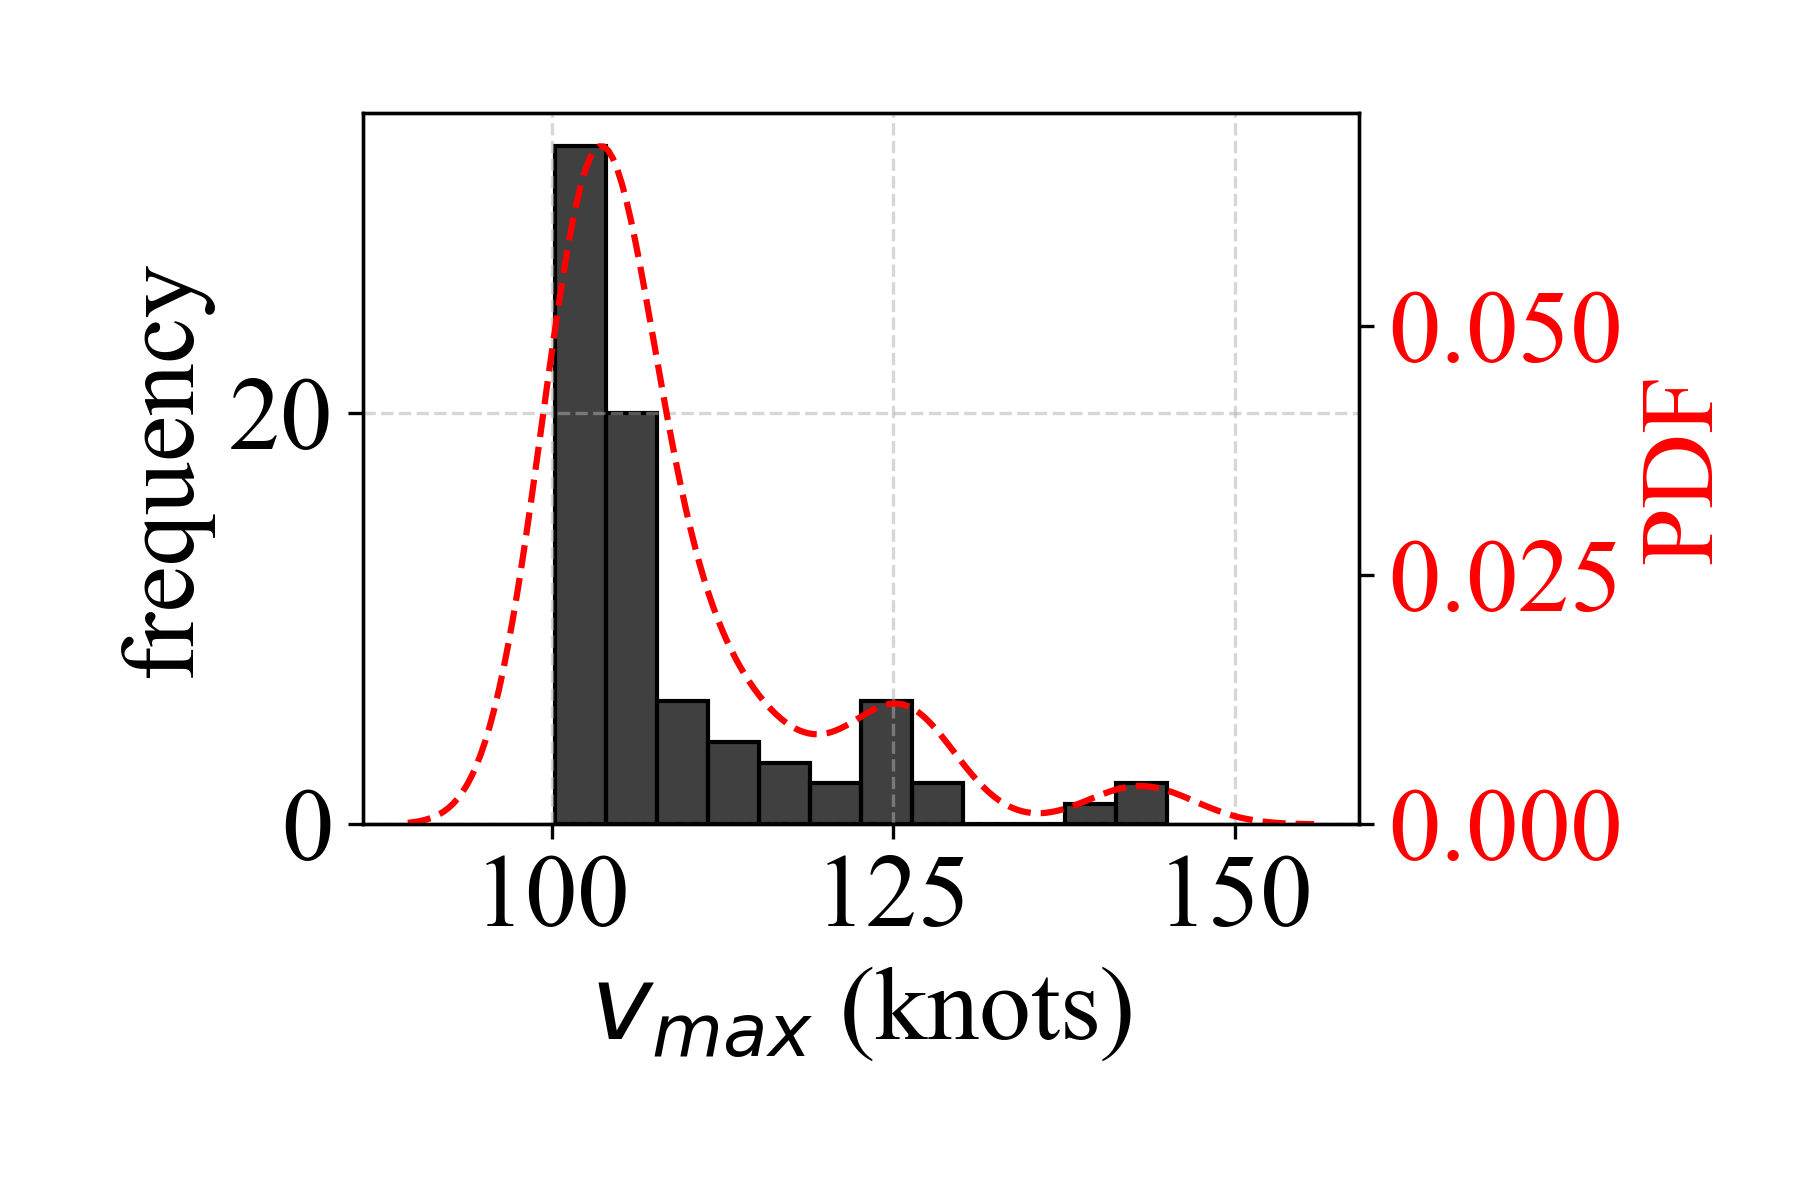
\includegraphics[clip, trim=0cm 0.7cm 0.1cm 0.5cm,width=\linewidth]{figures/Wm_kde.png}
        \caption{}
        % \label{fig:loss_scen}
    \end{subfigure}
    \hspace*{\fill}
    \vspace{-10pt}
    \caption{KDE of a) $R_{v_{max}}$, b) $R_s$, and c) $v_{max}$ estimated from the actual hurricanes that occurred in the USA~(1851--2012).} 
    \label{fig:three graphs}
\end{figure}

\subsubsection{Storm Surge Model}
In this work, we use SLOSH (Sea, Lake, and Overland Surge from Hurricanes) model to generate probabilistic storm surge scenarios. SLOSH is a numerical storm surge model that provides surge heights around the coastal regions from historical or hypothetical hurricanes based on parameters such as atmospheric pressure, hurricane tracks, forward speed, and so forth~\cite{glahn2009role}. It was developed by National Oceanic and Atmospheric Administration (NOAA) and is currently being used by several federal agencies, including the national hurricane center (NHC) and the federal emergency management agency (FEMA), for flood advisories and evacuation. Furthermore, NHC provides a SLOSH Display Package (SDP) tool in which users can generate flooding scenarios based on the direction, forward speed, and intensity of the hurricane followed by the sea tide level~\cite{SDP}. The provided surge heights are above the elevation referenced in the North American Vertical Datum of 1988 (NAV88). The tool also has an added functionality to subtract land elevations so that the surge level is referenced above the ground level. Details on the SDP tool and other surge-related products from NOAA can be found at~\cite{SDP}. 

SDP contains several coastal basins on which surge scenarios can be created. Furthermore, SDP provides two different surge analyses based on hurricane simulations: Maximum Envelope of Water (MEOW) and Maximum of the MEOWs (MOM). The MEOWs reflect the worst-case snapshots of the storm surge for hurricanes of particular intensity and forward direction but with different landfall locations. This work uses MEOW for storm surge scenarios to identify potential flooding locations. The MEOW scenarios from SDP provide the inundation level for each defined grid in a basin. Let $\mathcal{X}_\mathcal{S}$ be the geographical coordinate of a substation $\mathcal{S}$. Then, we define $\mathcal{X}^\mathcal{B}_{\mathcal{S}, h}$ as the inundation level, $h$, for substation $\mathcal{S}$ situated at $\mathcal{X}$ for basin $\mathcal{B}$. Since the inundation level is spatially distributed, the expected value of inundation around 0.5 miles of $\mathcal{X}_\mathcal{S}$ is assumed to be $\mathcal{X}^\mathcal{B}_{\mathcal{S}, h}$. 

\subsubsection{Impact Model}
Combined, the hurricane and storm surge creates a spatiotemporal effect on the power grid. The spatiotemporal impact of hurricanes on the power grid is generally guided by the fragility curves of the transmission lines~\cite{7801854}. Let $\Gamma_{l}^{t,\zeta}$ be the maximum wind speed on line $l$ at time step $t$ due to a hurricane traversing in track $\zeta$. Then the outage probability of line $l$ at time step $t$ due to a hurricane traversing in track $\zeta$ is given by (\ref{eq:hurricane_outage})      
\vspace{-1em}
\begin{equation}
\small
\begin{aligned}
&\mathbb{P}_{out}^{t,\zeta}(l)= \begin{dcases} 0 & \Gamma_{l}^{t,\zeta} < v_{cri} \\
\frac{\Gamma_{l}^{t,\zeta} - v_{cri}}{v_{col} - v_{cri}}  & v_{cri} \leq \Gamma_{l}^{t,\zeta} < v_{col} \\
1 & \Gamma_{l}^{t,\zeta} \geq v_{col} \end{dcases} \\
\end{aligned}
\label{eq:hurricane_outage}
\end{equation}

\noindent
where $v_{cri}$ = 48.59 knots and $v_{col}$ = 106.91 knots are the critical wind speed beyond which a transmission line is affected by the hurricane and the wind speed at which the transmission line collapses, respectively~\cite{9917119}. If $\delta_{l}^{t,\zeta} \in \{0,1\}$ denotes the line status of line $l$ at time $t$ for hurricane in track $\zeta$, then $\delta_{l}^{t + 1,\zeta} \leq  \delta_{l}^{t,\zeta}$. This ensures that if a line $l$ experiences an outage at time $t$, it remains out of service for the remaining duration of the hurricane.    

The impact assessment from storm surges can be modeled similarly by defining the outage probability of substations. Although FEMA has provided a general fragility level for substations in their HAZUS tool~\cite{hazus_flood}, we relax the curve through Weibull stretched exponential function as the substations around coasts have some hardening measures already in place. Hence, the outage probability of a substation $\mathcal{S}$ for a given inundation level $h$ at each basin $\mathcal{B}$ is given by (\ref{eq:flood_outage})

\vspace{-1em}
\begin{equation} 
\small
\mathbb{P}^{\mathcal{S}}_{out}(\mathcal{X}^\mathcal{B}_{\mathcal{S}, h}) = 1 - exp\left[- {\left(\frac{\mathcal{X}^\mathcal{B}_{\mathcal{S}, h}}{a}\right)^b}\right] \\
\label{eq:flood_outage}
\end{equation}

\noindent
where $a\in \mathbb{R}^+$ and $b>2$ are known constants and determine the shape of the fragility curve. When a substation is flooded and deemed out-of-service, all transmission lines connected to and from the substation are disconnected. If $\delta_{l,\mathcal{S}}^{t,\zeta} \in \{0,1\}$ denotes the line status of line $l$ connected to substation $\mathcal{S}$ at time $t$ for hurricane in track $\zeta$, then $\delta_{l, \mathcal{S}}^{t + 1,\zeta} \leq  \delta_{l,\mathcal{S}}^{t,\zeta}$. This ensures that if a line $l$ experiences an outage at time $t$ due to a storm surge, it remains out of service for the remaining event duration. 
When simulating storm surges as an effect of hurricanes, it is important to avoid the redundancy of impact that both transmission line and substation outages can have on the power grid. Let $\mathcal{L}^t_\mathcal{H}$ be the set of lines affected by hurricanes and $\mathcal{L}^t_\mathcal{S}$ be the set of lines out of service due to a flooded substation at time $t$. Then, the total number of lines affected by the compound effect of the hurricane and substations inundation due to storm surge is given by $\mathcal{L}^t_\mathcal{H} \cup \mathcal{L}^t_\mathcal{S}$.  


\subsection{Event Generation and Impact Assessment Framework}
Fig.~\ref{fig:overall_architecture} shows the overall architecture of the event generation and impact assessment process. First, synthetic hurricane tracks were generated based on historical data from IBTrACS. The hurricane impact model is then used to obtain the wind speed experienced by each transmission line. Similarly, flooding scenarios are obtained from SLOSH basins for the given characteristic of the hurricane. The fragility function defined in (\ref{eq:hurricane_outage}) and (\ref{eq:flood_outage}) provides the outage probability of transmission lines due to hurricanes and the outage probability of substations due to coastal flood inundation. Finally, Monte Carlo simulations (MCS) are conducted to obtain the probabilistic loss for the system. All flood scenarios are considered equally likely. The final spatiotemporal system-level loss metric for each time step is the obtained. The loss metric is the expected value of the loss obtained for the hurricane track and the flood basin for that particular time step.


\begin{figure}[t]
    \centering
    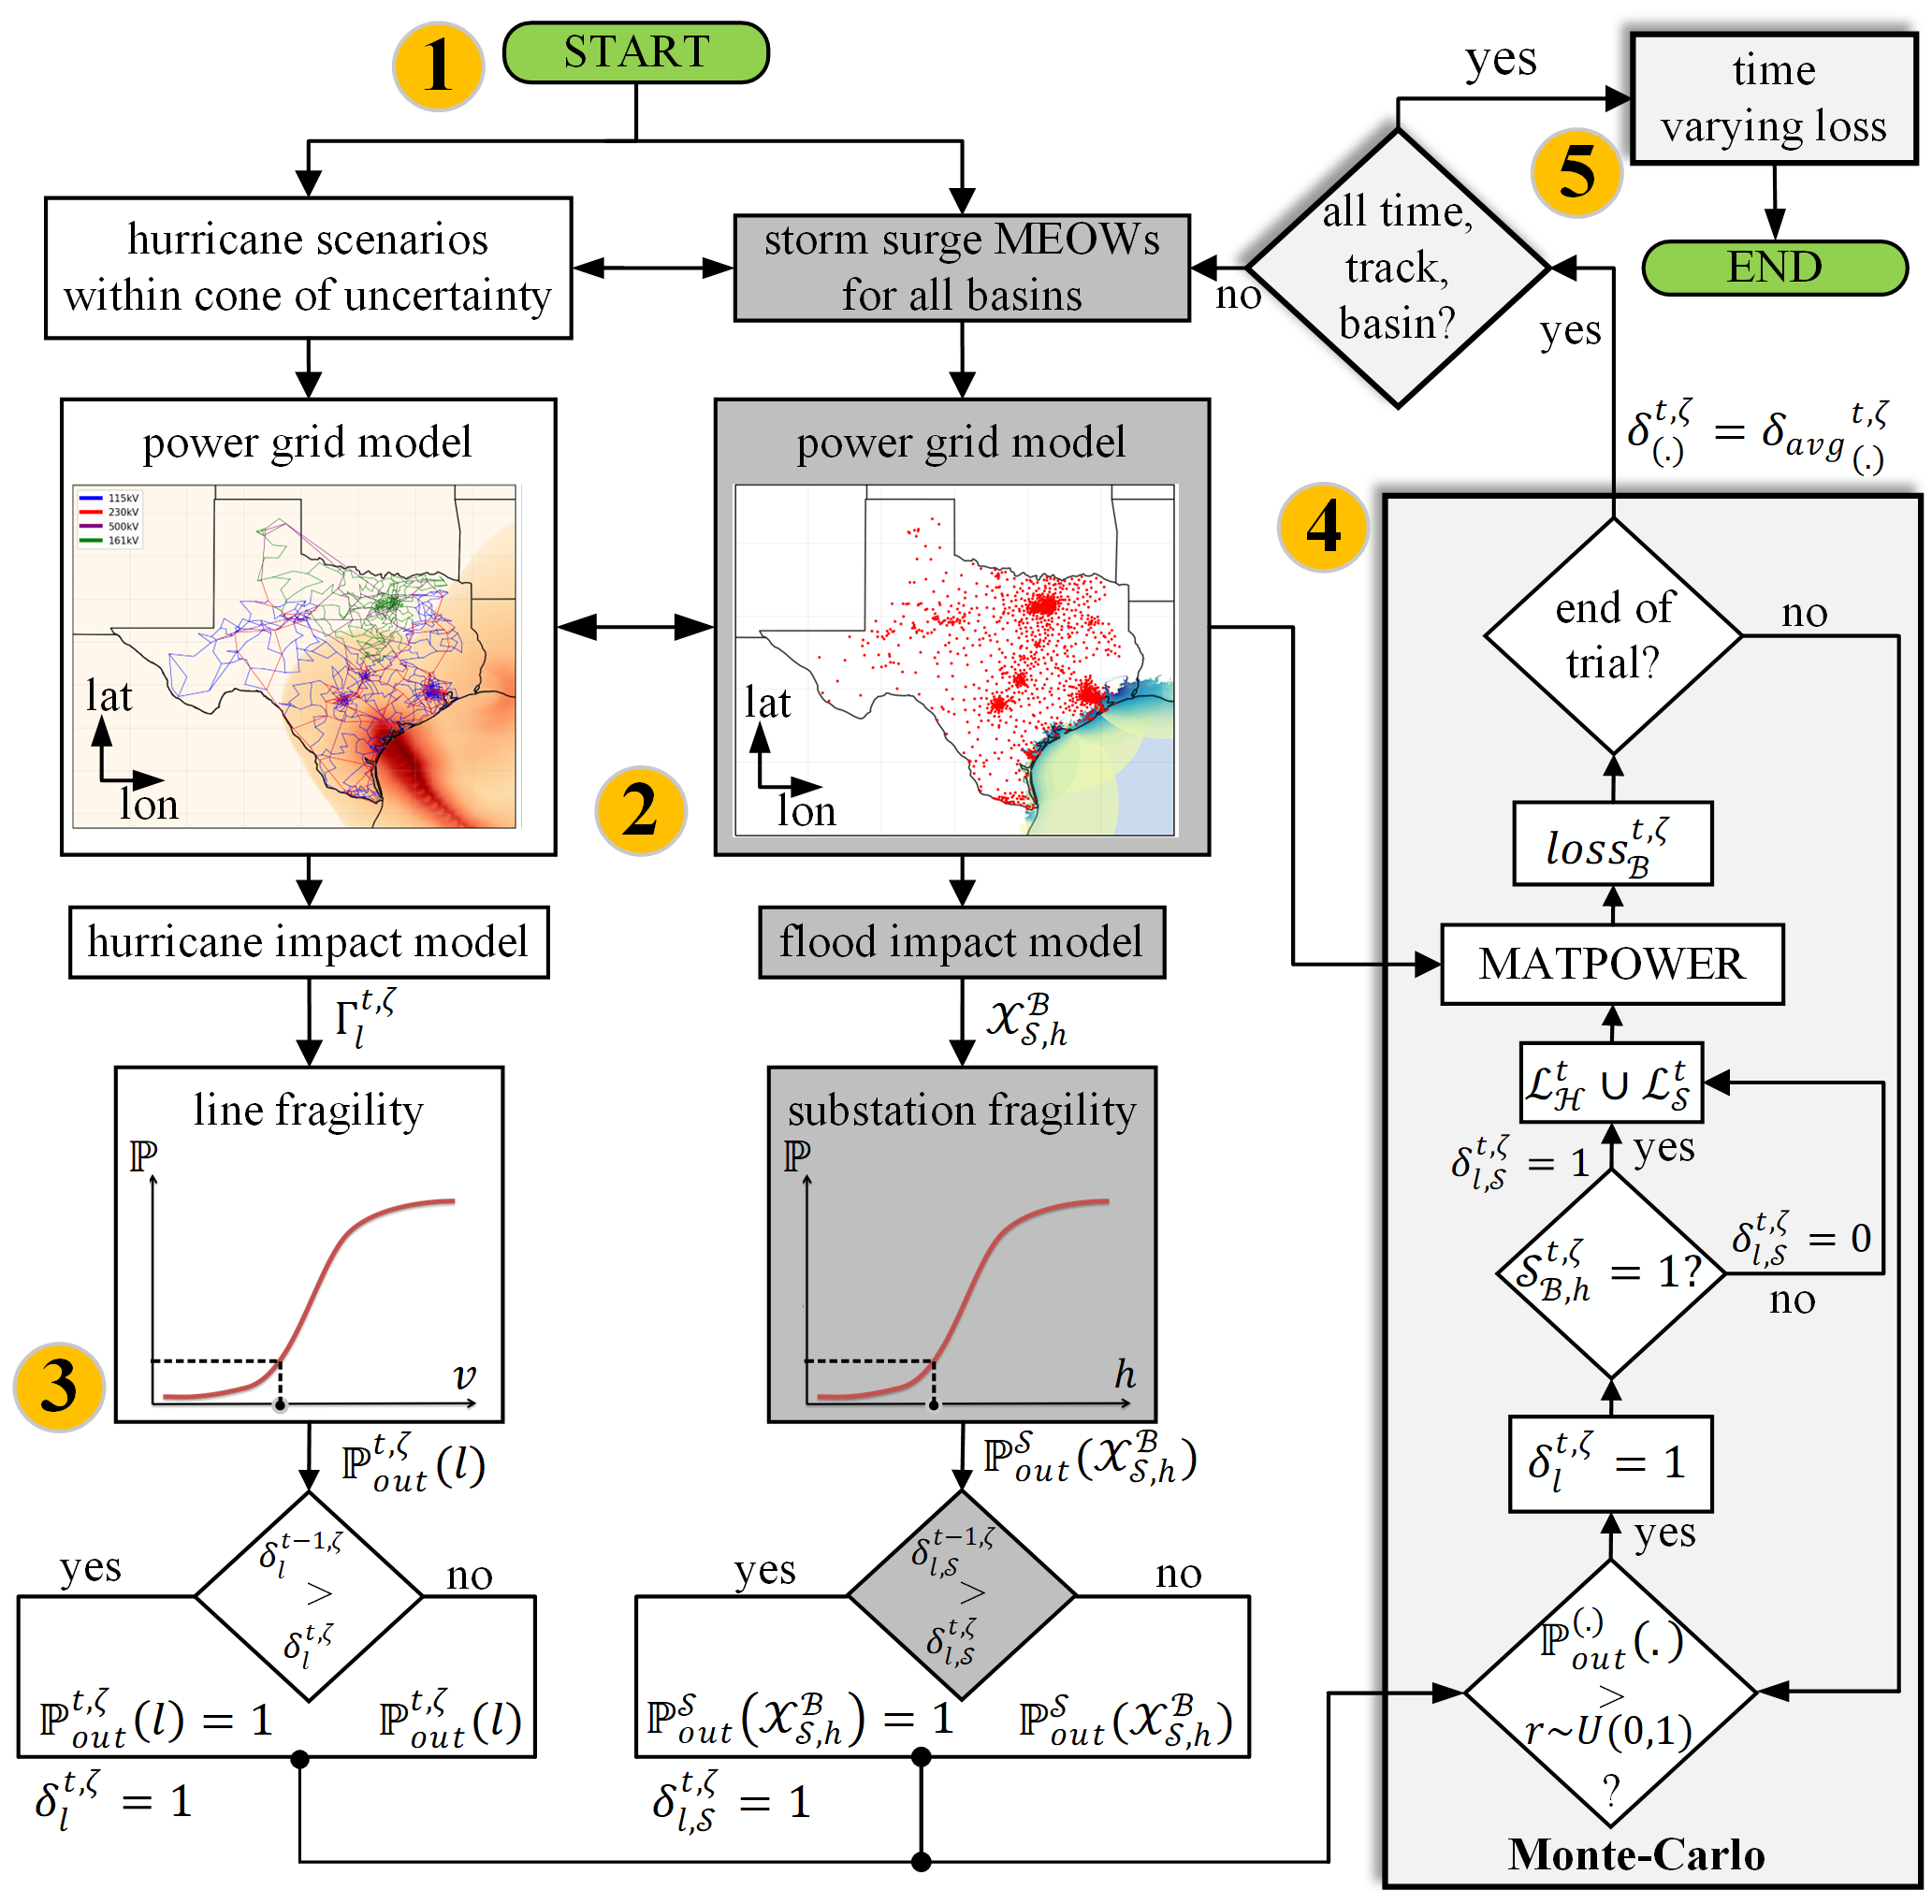
\includegraphics[width=0.7\textwidth]{figures/overall_framework.png}
   \caption{Overall architecture for generating hurricane and storm surge scenarios and grid impact assessment.}
    \label{fig:overall_architecture}
    \vspace{-5pt}
\end{figure}

\subsubsection{Hurricane and Storm Surge Scenario Generation}
The geographical data and parameters are obtained for Hurricane Harvey, that hit the coast of Texas in August 2017 using IBTrACS. Synthetic hurricane tracks are obtained by perturbing several characteristics of Hurricane Harvey, such as a shift in the initial point of origin, the amplitude of translational speed, bearing angle, landfall decay, etc. The synthetic tracks are obtained from the Climate adaptation (CLIMADA) tool. CLIMADA is a probabilistic natural catastrophe damage model that facilitates climate-based simulations~\cite{Climada}. CLIMADA can generate synthetic tracks in IBTrACS format based on the above perturbations. To synchronize the time steps for the entire duration of the hurricanes, the data is observed every two hours, and the hurricane wind field is generated for each $t$ using (\ref{eq:static_eq}). Fig.~\ref{fig:static_harvey} shows the synthetic tracks generated from CLIMADA, and the track with a solid line represents the actual track of Hurricane Harvey from IBTrACS. NOAA predicts that 7 out of 10 times, the estimated hurricane track is within the cone of uncertainty~\cite{NOAA_uncertainty}. Hence, five synthetic tracks are selected to be within the cone of uncertainty when forecasted over 120 hours of landfall, i.e., within 240 nmi as per~\cite{NOAA_uncertainty}.   

\begin{figure}[t]
    \centering
        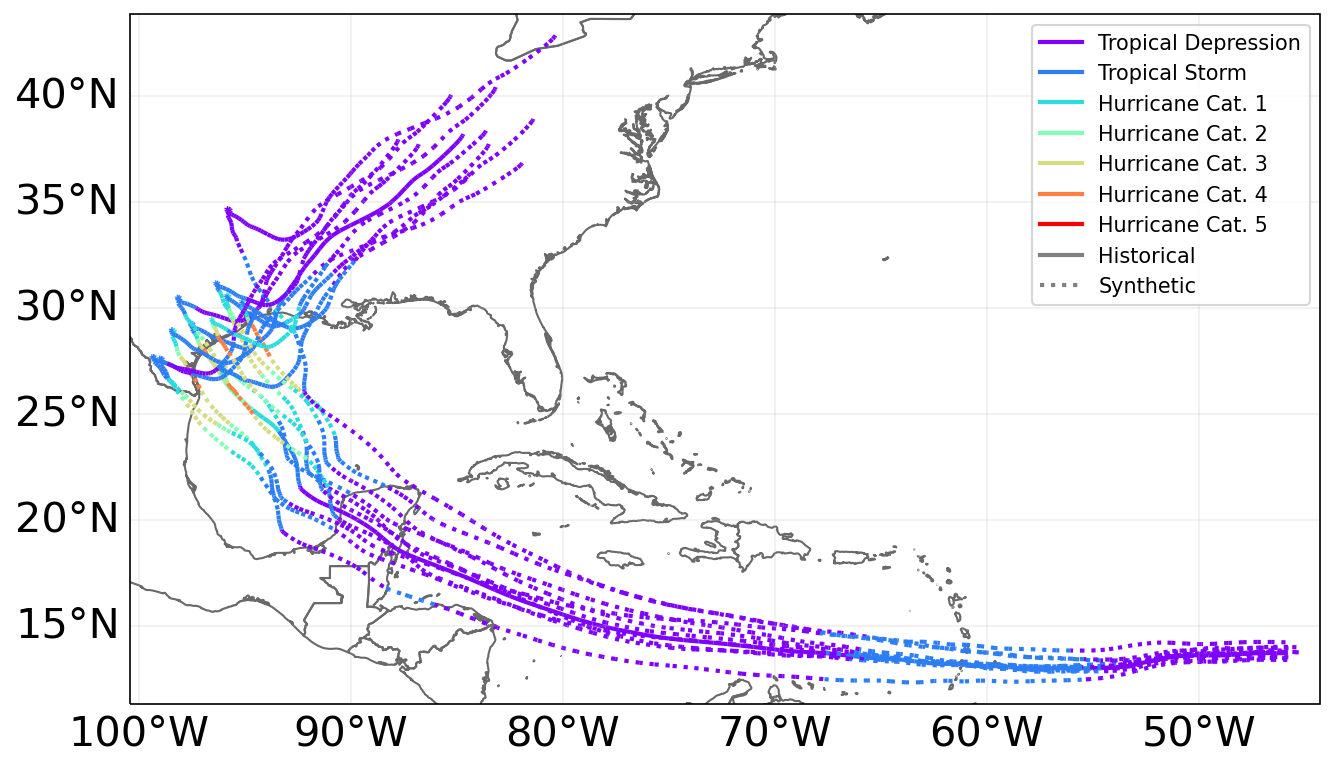
\includegraphics[width=0.7\textwidth]{figures/synthetic_tracks.png}
        \caption{Hurricane Harvey track and other synthetic tracks obtained from CLIMADA~\cite{Climada}.}
        \label{fig:static_harvey}
\end{figure}

For storm surge assessment, five different Texas basins are selected; $\mathcal{B} \in$ \{Matagorda, Corpus, Galveston, Laguna, Sabine\}. MEOW scenarios are obtained for all five basins for category 4 hurricanes moving in the northwest direction with a translational speed of 10-15 miles per hour and mean to high tide conditions. One major drawback of using MEOW maps is they are snapshots of the storm surge and carry no time information. However, we can assume that the components are not inundated until the hurricane approaches. Hence, we assign an activation flag for each component per basin at each time step. 


\subsubsection{Power Systems Impact Assessment}
This work uses a synthetic 2000-bus Texas power grid model to identify the compound probabilistic impact of hurricane and storm surges on the power grid~\cite{7725528}. The grid model maps the synthetic buses, substations, and transmission lines on the geographical footprint of Texas. There are 1250 substations and 1918 transmission lines at 4 different voltage levels --- 115 kV, 161 kV, 230 kV, and 500 kV. The total generation capacity of the system is 96291.5 megawatts (MW), and there are 1125 load units with a total size of 67109.2 MW. When the hurricane moves inland, $\Gamma_{l}^{t,\zeta}$ is obtained for each $l$ and $\mathcal{X}^\mathcal{B}_{\mathcal{S}, h}$ is obtained for each $\mathcal{S}$ from the MEOW maps. It is assumed that all substations at the coast are elevated at a level of 3 ft from the ground level. Fig.~\ref{fig:hurricane_flood_scenario} shows the wind field of Hurricane Harvey and MEOW maps on five different basins on the footprint of Texas.     

For each $\zeta$, $\mathcal{B}$, and $t$, MCS is performed for several trials. For each trial, $\mathbb{P}_{out}^{t,\zeta}(l)$ and $\mathbb{P}^{\mathcal{S}}_{out}(\mathcal{X}^\mathcal{B}_{\mathcal{S}, h})$ is compared with a uniform random number, $r\sim U(0,1)$, to identify $\mathcal{L}^t_\mathcal{H} \cup \mathcal{L}^t_\mathcal{S}$. As discussed before, MEOW maps are time-independent. However, we define an activation flag $\mathcal{S}^{t, \zeta}_{\mathcal{B}, h} \in \{0,1\}$ such that $\mathcal{S}^{t, \zeta}_{\mathcal{B},h} = 1$ makes the substation $\mathcal{S}$ inundated with depth $h$ above the ground elevation for hurricane track $\zeta$, SLOSH basin $\mathcal{B}$, and time $t$. In this work, we do not model any drainage system, and hence it is assumed that for future time steps $t+1$ the inundation level is the same. The objective here is to identify the time stamp when the substation gets flooded to analyze the compound spatiotemporal impact of two different hazards at that time step. The information, $\mathcal{L}^t_\mathcal{H} \cup \mathcal{L}^t_\mathcal{S}$, is then sent to the power grid simulator to remove the respective branches from the system. Finally, the loss for the particular $t$ is observed as the total load disconnected from the main grid. The MCS trial is conducted until the loss converges to some value.

We assume that the inundation scenarios for each $\mathcal{B}$ and each of the hurricane tracks $\zeta$ are equally likely. If $N_\zeta$ is the total number of tracks under consideration and $N_\mathcal{B}$ is the total number of basins, then the system level load loss at each time step $t$ is given by (\ref{eq:final_loss})

\begin{equation}
\small
    loss_t = \frac{1}{N_\zeta \times N_\mathcal{B}}\sum_{\zeta = 1}^{N_\zeta}{\sum_{\mathcal{B}} {loss_{\mathcal{B}}^{t,\zeta}}}
    \label{eq:final_loss}
\end{equation}

\begin{figure}[!ht!]
    \centering
    \begin{subfigure}[t]{0.7\textwidth}
        \centering
        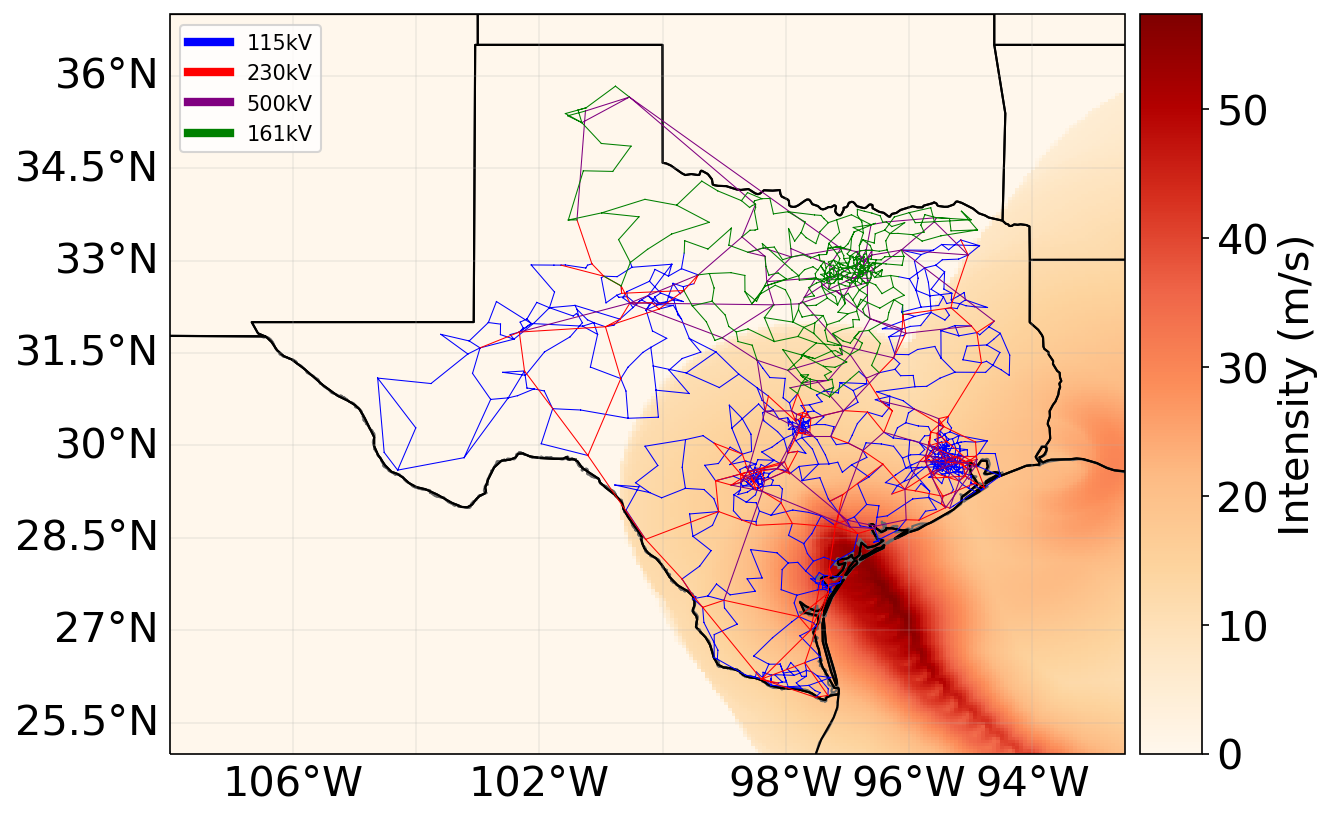
\includegraphics[width=0.8\linewidth]{figures/windfield_harvey_climada.png}
        \caption{}
        \label{fig:dynamic_harvey}
        % \vspace{-5pt}
    \end{subfigure}
    \begin{subfigure}[t]{0.7\textwidth}
        \centering
        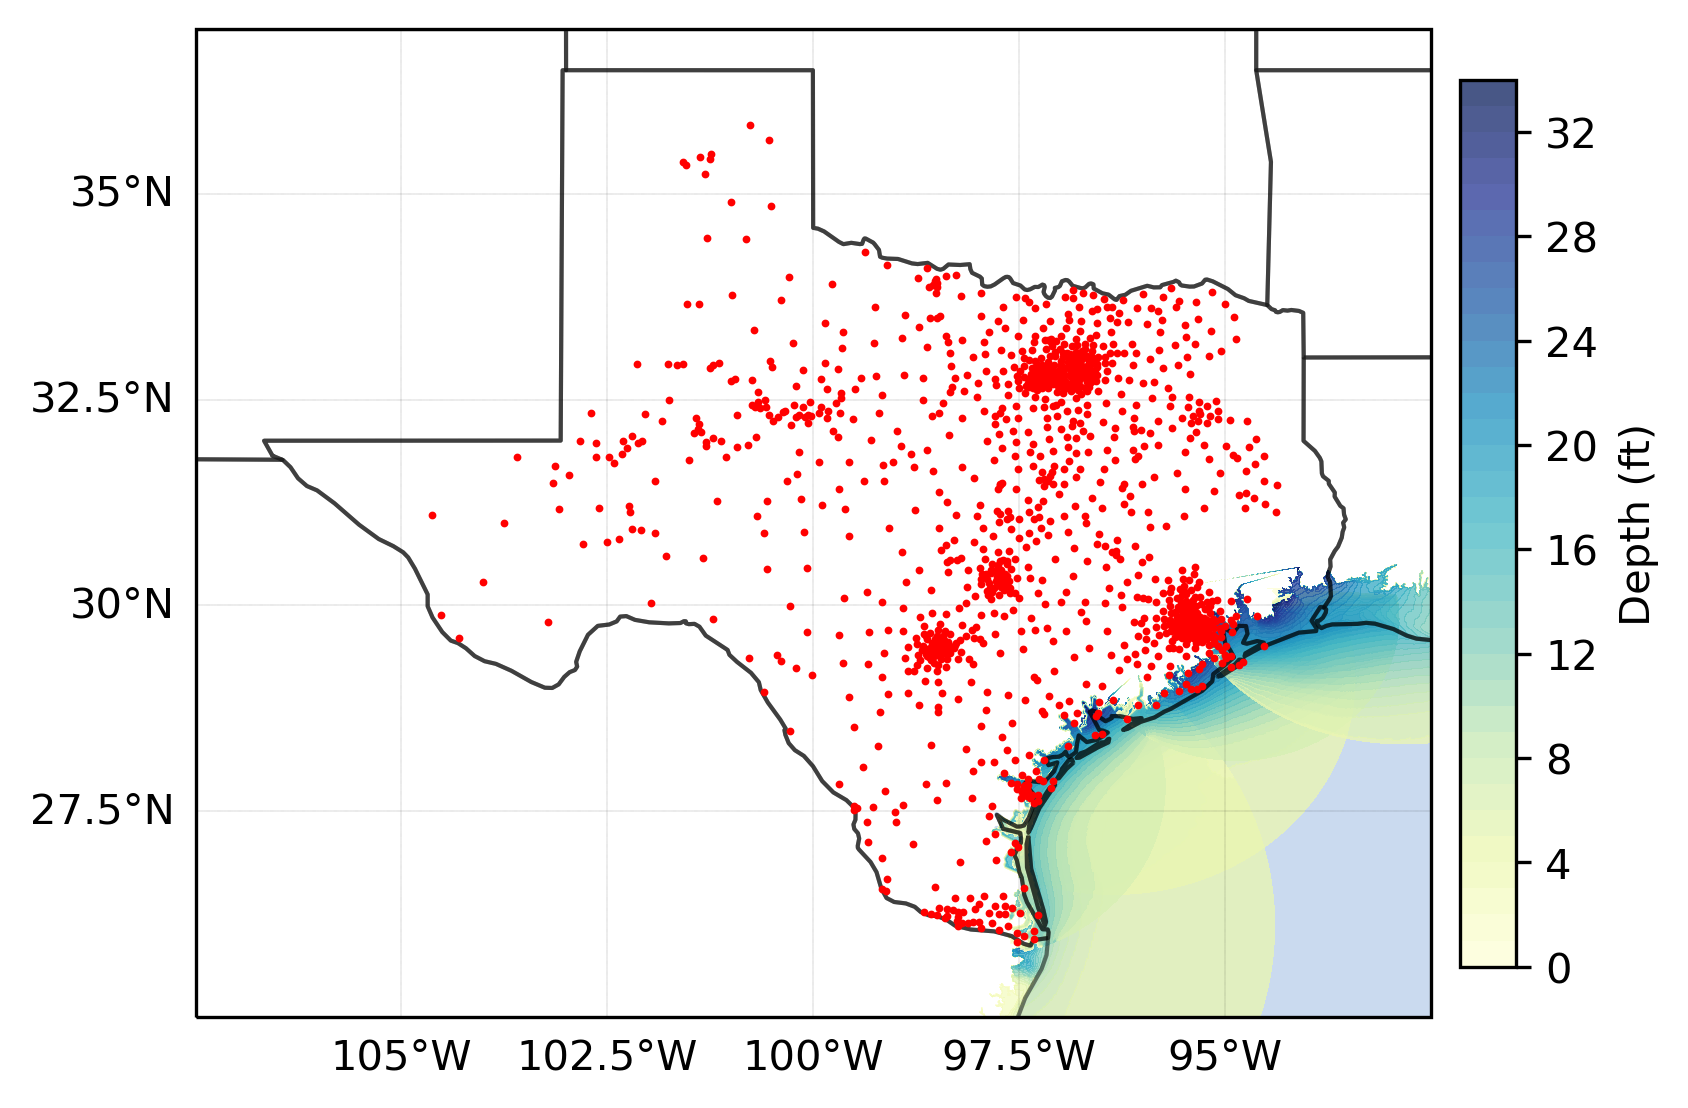
\includegraphics[width=0.8\linewidth]{figures/sub_flood.png}
        \caption{}
        \label{fig:flood_scenario}
        % \vspace{-5pt}
    \end{subfigure}
    \caption{a) Wind field of Hurricane Harvey and b) Substation flooding scenario, above ground level, for Texas basins.} 
    \label{fig:hurricane_flood_scenario}
\end{figure}

\subsection{Preliminary Research Results}
The hurricane data is obtained from IBTrACS~\cite{Knapp2010}, and synthetic hurricanes are generated using CLIMADA~\cite{Climada} in Python. SDP~\cite{SDP} is used to obtain the MEOW maps for Texas basins. The power grid is modeled in MATPOWER 7.1~\cite{5491276}, and MCS on the power grid model is conducted in MATLAB R2021a.  
From the IBTrACS, the hurricane's initial location is in the North Atlantic Ocean, which is observed at $``2017-08-16~06:00:00''$ and hence creates no impact on the power grid. Thus, the simulation for the impact assessment begins at the $100^{th}$ time step, i.e., at the advisory of $``2017-08-24~12:00:00''$. To avoid any confusion, this timestamp is referred to as $t=0$ hours for the rest of the paper. Fig.~\ref{fig:line_outage_probability} shows the outage probability of a set of transmission lines due to the original Hurricane Harvey track. It can be observed that with the moving nature and intensity of the hurricane, the outage probability of each line changes. The probability is maximum when the line experiences wind speed closer to $v_{col}$ and gradually decreases as the hurricane decays while moving inland. Fig.~\ref{fig:substation_outage_probability} represents the outage probability of substations for five different Texas basins. It is seen that the substation's vulnerability depends on the location and basin.

\begin{figure}[!h!]
    \centering
    \begin{subfigure}[t]{0.47\textwidth}
        \centering
        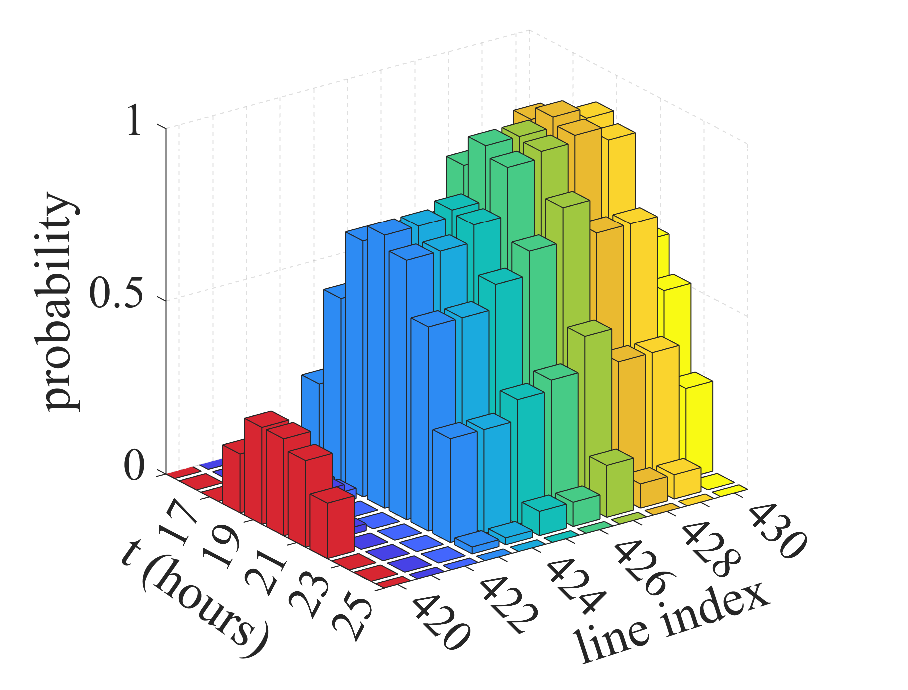
\includegraphics[width=\linewidth]{figures/outage_probability_line_.eps}
        \caption{}
        \label{fig:line_outage_probability}    
    \end{subfigure}
    \hspace*{\fill}
    \begin{subfigure}[t]{0.47\textwidth}
        \centering
        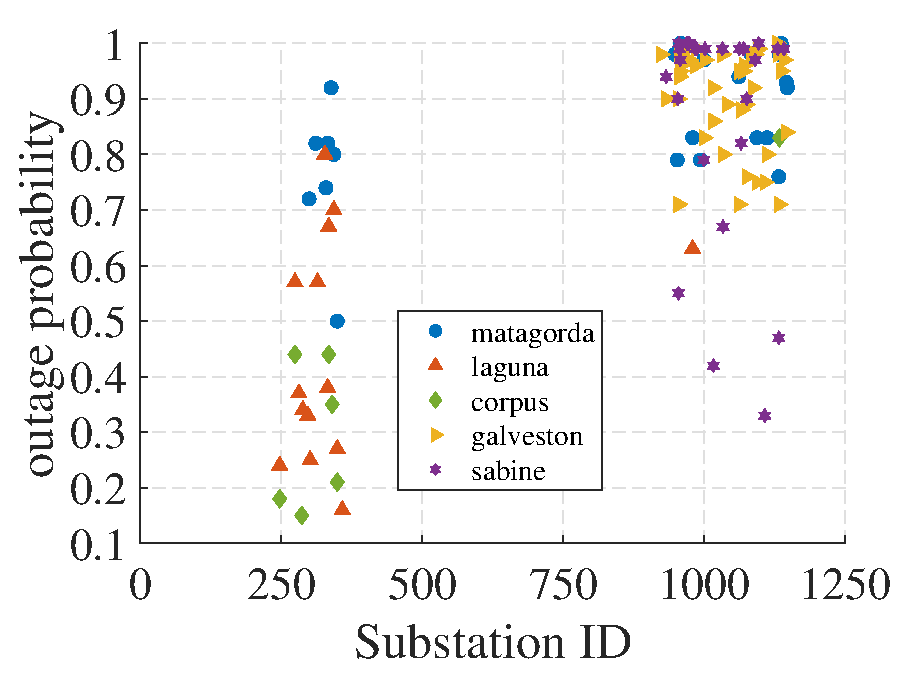
\includegraphics[width=\linewidth]{figures/outage_probability_substation_.eps}
        \caption{}
        \label{fig:substation_outage_probability}
    \end{subfigure}
    \caption{a) Line outage probability for selected lines and the original Harvey's track. b) Substation outage probability for all storm surge scenarios.} 
    \vspace{-10pt}
    \label{fig:hurricane_flood_outages}
\end{figure}

It was found that 800 Monte Carlo trials are enough to achieve convergence for any simulation case~\cite{9917119}. Hence, for each $\zeta$, $\mathcal{B}$, and $t$, 800 Monte Carlo trials are conducted. Fig.~\ref{fig:hurricane_flood_compound} shows the comparison of losses when considering the impact of the hurricane alone with the compound effect of the hurricane and the coastal flood for $\zeta=1$. It can be observed that considering substation flooding scenarios incur an additional loss of $250~MW$ by $t=50$ hours due to substation outages.   

\begin{figure}
    \centering
    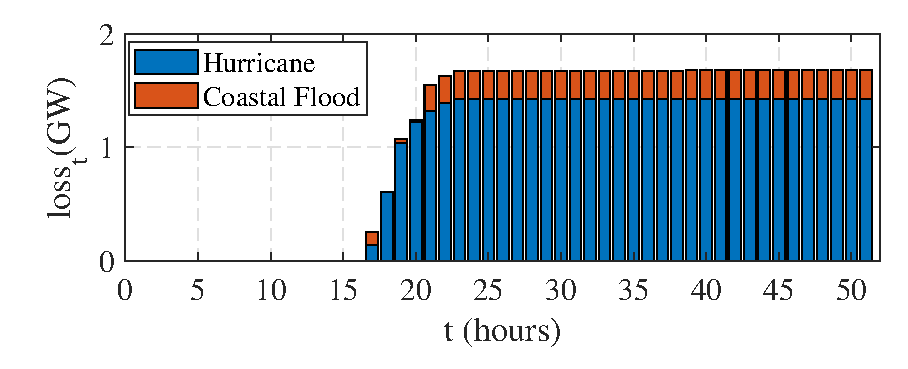
\includegraphics[width=0.7\textwidth]{figures/hurricanevsflood.eps}
    \caption{Overall loss comparison between the impact of hurricane alone and the compound impact of the hurricane and coastal flood for $\zeta = 1$.}
    \label{fig:hurricane_flood_compound}
\end{figure}

Fig.~\ref{fig:final_losses} represents the spatiotemporal loss for the compound impact of hurricane and storm surge. The dashed curves represent the loss for all basins for each track, whereas the solid blue curve represents $loss_t$ obtained from (\ref{eq:final_loss}). The loss is not incurred until $t=12$ for any $\zeta$ under consideration, and the increase is significant once the hurricane moves inland, followed by the compounded impact of storm surge. The loss increases from $loss_{12} = 9.4072$ MW to $loss_{22} = 5536.1$ MW before saturating at $loss_{40} = 6761.97$ MW as the intensity of the extreme events decreases.  

\begin{figure}[!h!]
    \centering
    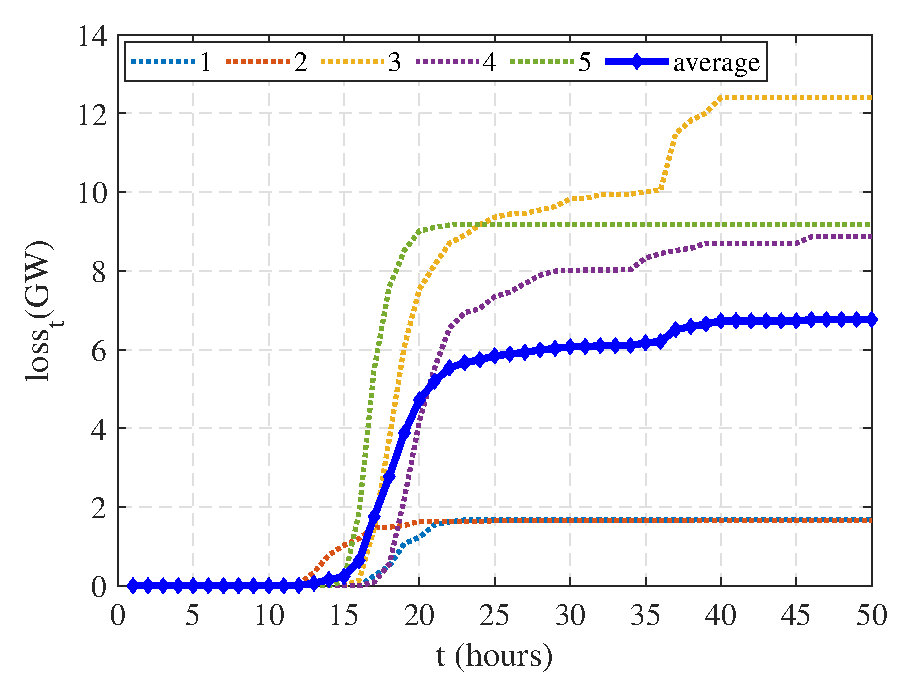
\includegraphics[width=0.7\textwidth]{figures/all_basin_losses.eps}
    \caption{Time-varying loss for each hurricane track. For each track, the loss at each time step also includes the expected value of loss over entire flood basins.}
    \label{fig:final_losses}
\end{figure}


\clearpage
\section{Future Works}\label{sec:future_Work}
The current work in progress aims at scaling the current resilience planning framework to solve large-scale optimization model in terms of resources, network, and scenario under consideration. As discussed in our existing work, the scenarios are time and space varying and hence such details are necessary to be incorporated in the planning model for better accuracy. Additionally, solving the extensive form of the problem is suffered by the curse of dimensionality. Hence, off-the-shelf solvers are more likely to crash or provide high optimality gap solutions when high dimensionalo extensive form of the model is fed to the solvers. Thus, solving a large-scale stochastic optimization problem has several challenges and is an active area of research that motivates us in our future work. In addition, operational planning strategies like defensive islanding would be studied to better prepare with the upcoming hurricane storms. Such proactive islanding method can prevent the propagation of cascading failure effects in the power system.

\subsection{Large-scale Resilience Planning Framework}
\subsubsection{Multiple-resource Resilience Planning using Scenario-based Dual Decomposition}
Our existing planning model plans for the DG siting and sizing problem for a range of stochastic wind events. However, the infrastructures planning problem can have multiple portfolio of resources including remote-controlled switches (RCS) and line hardening measures. There are existing works using several other planning measures as such~\cite{7514755}. However, as discussed earlier, such methods plan for the expected events but not for HILP events. The objective of this task is to formulate a planning model with multiple resources and observe the trade-off of planning among these multiple resources considering budget constraints. A dual decomposition-based algorithm will be studied to solve the scenario-based sub-problems in parallel by leveraging high-performance computing (HPC) platforms. Although such algorithms are heuristically driven, several convergence  and bounding guarantees exist in the literature for such algorithms~\cite{boland2018combining}.   

\subsubsection{Hub and Spoke Architecture for Scalable and Parallel Implementation of Stochastic Optimization}
Although parallel algorithms are faster in solving the stochastic optimization problem they can run into bottlenecks when individual sub-problems are hard to solve. In such a case, communication overhead can outweigh the parallel speedup. Such problems can rather take more time than serial methods as subproblems that have finished their work need to wait for other subproblems that have not. Hence, the objective of this task is to explore asynchronous parallel algorithm based on hub and spoke architecture as suggested in~\cite{knueven2020parallel}. When solved in hub and spoke architecture, the problems can be independently solved with less or no communication. This asynchronous problem-solving behavior increases the parallel speedup significantly. 

\subsection{Defensive Islanding and Restoration of Electric Power Systems Against Extreme Weather Events}
Extreme weather event, such as hurricane and storm surge, can have devastating impacts on the power grid and can result in cascading failures of the resources if not handled properly. During an upcoming storm, it is typically difficult to address the operational decisions considering the timescale of the events and resources required. However, it is possible to minimize the impact of these events if the grid is splitted into multiple self-sustaining islands ahead of the event. There are some existing works proposing the idea of defensive islanding. However, the event scenarios in these works are non-realistic as the spatiotemporal impact of these events are not considered. The aim of this work is to propose a defensive islanding strategy to minimize the spatiotemporal impact of extreme weather events. Furthermore, restorative actions will also be implemented once the event settles after some time.    

%\begin{comment}
\clearpage
\subsection{Timeline}
The time-line for the research efforts as detailed in Section~\ref{sec:future_Work} is shown in Fig. \ref{fig:time}.

\begin{figure}[h!]
\centering
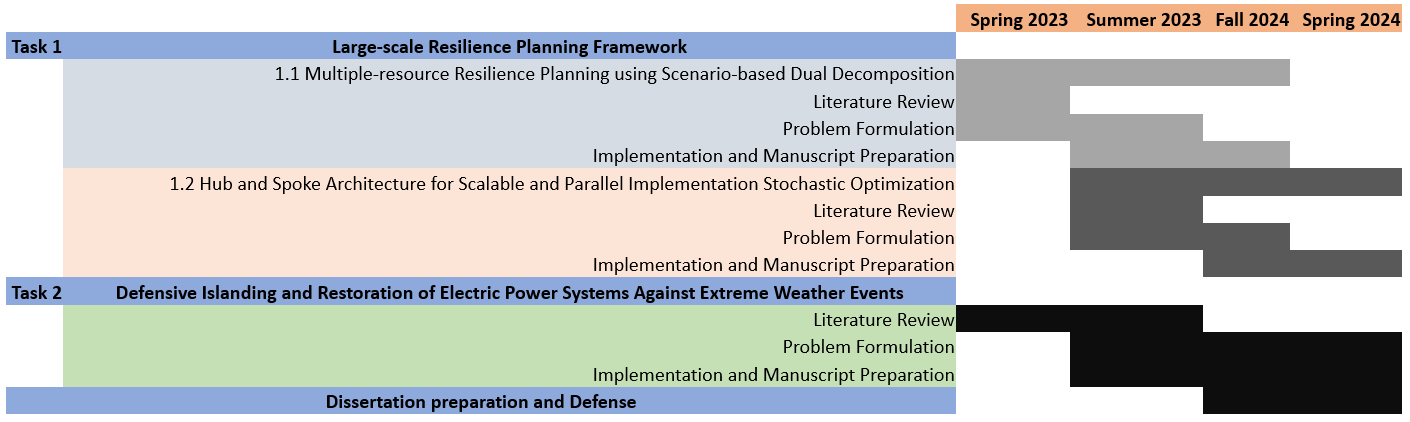
\includegraphics[width=\linewidth]{figures/timeline.PNG}
  \vspace{-0.2 cm}
  \caption{\small Gantt chart showing execution plan for future works.}
\label{fig:time}
\end{figure}



\newpage
\section{Biography}
\section{Biography}
\small
Aryan Ritwajeet Jha received the B.E. degree in Electrical and Electronics Engineering from the Birla Institute of Technology and Science (BITS) Pilani, India, in 2020. He is currently pursuing his Ph.D. in Electrical Engineering at Washington State University, Pullman, WA, USA. His research interests include power distribution system optimization, scalable decomposition algorithms for large-scale non-linear optimization and optimization solvers.
\singlespacing

\subsection{Publications}
\small
\begin{enumerate}
    \item [Publications to be updated based on research progress]
\end{enumerate}


\clearpage
\subsection{Course Work}
% \usepackage{booktabs}
\begin{table}[h!]
\centering
\setlength{\tabcolsep}{4pt}
%\caption{}
\label{tab:my-table}
\begin{adjustbox}{width=1\textwidth,center=\textwidth}
\begin{tabular}{@{}l|l|l|l@{}}
\toprule
Course Number and Name                          & Semester       & Instructor                     & Grade \\ \midrule

E\_E 507 Random Processes in Engineering        & Fall 2022      & Prof. Sandip Roy               & A    \\
E\_E 521 Analysis of Power Systems              & Fall 2022      & Prof. Noel Schulz              & A    \\
E\_E 523 Power Systems Stability                & Spring 2023    & Prof. Mani V. Venkatasubramanian & A   \\
MATH 564 Convex and Nonlinear Optimization      & Fall 2023      & Prof. Tom Asaki                & A    \\
MATH 565 Nonsmooth Analysis and Optimization    & Spring 2024    & Prof. Tom Asaki                & A-   \\
MATH 567 Integer and Combinatorial Optimization\textsuperscript{\ref{note2}} & Spring 2025    & Prof. Bala Krishnamoorthy & I \\
CPT\_S 530 Numerical Analysis\textsuperscript{\ref{note1}} & Fall 2025 & Prof. Alexander Panchenko & \\
E\_E 582 Electrical Systems Modelling and Simulation\textsuperscript{\ref{note1}} & Fall 2025 & Prof. Seyedmilad Ebrahimi & \\

E\_E 595 Directed Study in Electrical Engineering\textsuperscript{\ref{note1}} & Fall 2025 & Prof. Rahul K. Gupta & \\ \bottomrule
\end{tabular}
\end{adjustbox}

\tablefootnote{\label{note1}currently taking this semester}
\tablefootnote{\label{note2}currently finishing some leftover work - NOT part of my prelims (Program of Study) or graduation requirements}

\end{table}



% BIBLIOGRAPHY %%%%%%%%%%%%%%%%%%%%%%%%%%%%%%%%%%%%%%%
\newpage

\bibliographystyle{IEEEtran}
\bibliography{ref.bib}
\end{document}
